\documentclass[12pt, a4paper]{report}
% \usepackage[vietnam]{babel}
\usepackage[utf8]{vietnam}
\usepackage{minted}
\usepackage{csvsimple}
\usepackage{cases}
% \usepackage{vntex}
%\usepackage[english,vietnam]{babel}
%\usepackage[utf8]{inputenc}
\usepackage{svg}
\usepackage{float}

%\usepackage[utf8]{inputenc}
%\usepackage[francais]{babel}
\usepackage{a4wide,amssymb,epsfig,latexsym,multicol,array,hhline,fancyhdr}

% \usepackage{amsmath}
\usepackage{amsfonts}
\usepackage{amssymb}
\usepackage{lastpage}
\usepackage[lined,boxed,commentsnumbered]{algorithm2e}
\usepackage{enumerate}
\usepackage{color}
\usepackage{graphicx}

% Standard graphics package
\usepackage{subcaption}
\usepackage{array}
\usepackage{tabularx, caption}
\usepackage{multirow}
\usepackage{multicol}
\usepackage{rotating}
\usepackage{graphics}
\usepackage[a4paper,left=3cm,right=2cm,top=2cm,bottom=2.8cm]{geometry}
\usepackage{setspace}
\usepackage{epsfig}
\usepackage{tikz}
\usepackage{indentfirst}
\usepackage{bkthesis}
\usetikzlibrary{arrows,snakes,backgrounds}
\usepackage[unicode]{hyperref}
%can file puenc.def trong thu muc goc de option [unicode] tao ra bookmark bang tieng Viet
\hypersetup{urlcolor=blue,linkcolor=black,citecolor=black,colorlinks=true} 
%\usepackage{pstcol} 								
% PSTricks with the standard color package

\newtheorem{theorem}{{\bf Theorem}}
\newtheorem{property}{{\bf Property}}
\newtheorem{proposition}{{\bf Proposition}}
\newtheorem{corollary}[proposition]{{\bf Corollary}}
\newtheorem{lemma}[proposition]{{\bf Lemma}}


%\usepackage{fancyhdr}
\setlength{\headheight}{40pt}
\pagestyle{fancy}
\fancyhead{} % clear all header fields
% \fancyhead[L]{
%  \begin{tabular}{rl}
%     \begin{picture}(25,15)(0,0)
%     \put(0,-8){
\includegraphics[width=8mm, height=8mm]{img/LogoBK.jpg}}
%     %\put(0,-8){\epsfig{width=10mm,figure=hcmut.eps}}
%   \end{picture}&
% 	%\includegraphics[width=8mm, height=8mm]{hcmut.png} & %
% 	\begin{tabular}{l}
% 		\textbf{\bf \ttfamily Trường Đại học Bách Khoa - ĐHQG TP.HCM}\\
% 		\textbf{\bf \ttfamily Khoa Khoa học \& Kỹ thuật Máy tính}
% 	\end{tabular} 	
%  \end{tabular}
% }
% \fancyhead[R]{
% 	\begin{tabular}{l}
% 		\tiny \bf \\
% 		\tiny \bf 
% 	\end{tabular}
% }
\fancyhead[LE, RO]{
	Hệ thống phòng Tổ chức - Hành chính
}
\fancyfoot{} % clear all footer fields
% \fancyfoot[L]{\scriptsize \ttfamily Hệ thống phòng Tổ chức - Hành chính}
% \fancyfoot[R]{\scriptsize \ttfamily Page {\thepage}/\pageref{LastPage}}
\fancyfoot[C]{{\thepage}}
\renewcommand{\headrulewidth}{0.3pt}
\renewcommand{\footrulewidth}{0.3pt}


%%%%%%%% create subsubsubsection %%%%%%%%%%%%%%%%%%%%%%
\setcounter{secnumdepth}{4}
\setcounter{tocdepth}{3}
\makeatletter
\newcounter {subsubsubsection}[subsubsection]
\renewcommand\thesubsubsubsection{\thesubsubsection .\@alph\c@subsubsubsection}
\newcommand\subsubsubsection{\@startsection{subsubsubsection}{4}{\z@}%
                                     {-3.25ex\@plus -1ex \@minus -.2ex}%
                                     {1.5ex \@plus .2ex}%
                                     {\normalfont\normalsize\bfseries}}
\newcommand*\l@subsubsubsection{\@dottedtocline{3}{10.0em}{4.1em}}
\newcommand*{\subsubsubsectionmark}[1]{}
\makeatother
%%%%%%%% end create subsubsubsection %%%%%%%%%%%%%%%%%%

\begin{document}
\usetikzlibrary{calc}

\begin{titlepage}
\begin{tikzpicture}[remember picture, overlay]
  \draw[line width = 2pt,color=blue] ($(current page.north west) + (2.15cm,-2.15cm)$) rectangle ($(current page.south east) + (-2.15cm,2.15cm)$);
   \draw[line width = 1pt,color=black] ($(current page.north west) + (2.0cm,-2.0cm)$) rectangle ($(current page.south east) + (-2.0cm,2.0cm)$);
\end{tikzpicture}
\begin{center}
\textbf{\large{ĐẠI HỌC QUỐC GIA TP.HCM}}\\
\textbf{\large{TRƯỜNG ĐẠI HỌC BÁCH KHOA}}\\
\textbf{\large{KHOA KHOA HỌC \& KỸ THUẬT MÁY TÍNH}}\\
- - - - - - - - - - - -
\end{center}

\vspace{0.5cm}
\begin{figure}[H]
\begin{center}

\includegraphics[width=3cm]{img/LogoBK.jpg}
\end{center}
\end{figure}
\vspace{0.5cm}

\begin{center}
\begin{tabular}{c}
\multicolumn{1}{c}{\textbf{{\Large LUẬN VĂN TỐT NGHIỆP ĐẠI HỌC}}}\\
~~\\
\hline
\\
\multicolumn{1}{c}{\textbf{{\Large XÂY DỰNG HỆ THỐNG THÔNG TIN}}}\\
\textbf{{\Large PHÒNG TỔ CHỨC - HÀNH CHÍNH}}\\\\
\hline
\\
\large{Ngành: Khoa học Máy tính}
\end{tabular}
\end{center}

\vspace{1cm}
\begin{table}[h!]
    \fontsize{15pt}{1}
    \centering
    \begin{tabular}{lll}
        \textbf{Hội đồng:} & \textbf{Khoa học Máy tính}\\
        \textbf{GVHD:} & \textbf{Th.S Nguyễn Thanh Tùng}\\
        \textbf{GVPB:} & \textbf{PGS.TS Trần Minh Quang}\\
\\
        \textbf{Sinh viên thực hiện:} & \textbf{Nguyễn Quốc Cường (1610372)}\\
        & \textbf{Nguyễn Hoàng Nam (1612115)}\\
        & \textbf{Nguyễn Xuân Thi (1613297)}\\
    \end{tabular}
\end{table}
\vspace{1.5cm}
\begin{center}
{\footnotesize TP. HỒ CHÍ MINH, THÁNG 08/2020}
\end{center}
\end{titlepage}
% \selectlanguage{vietnamese}
\begin{declaration}
Chúng tôi xin cam đoan rằng đề tài luận văn tốt nghiệp: "Xây dựng Hệ thống Tổ chức - Hành chính" là do chúng tôi thực hiện dưới sự hướng dẫn của Th.S Nguyễn Thanh Tùng. Tất cả các tham khảo từ các công trình khác đều được ghi rõ trong mục "Tài liệu tham khảo". Nội dung của luận văn này chưa từng được công bố trước đây dưới bất kì hình thức nào. Nếu có bất kì sai phạm nào, chúng tôi xin chịu hoàn toàn trách nhiệm trước Ban Chủ nhiệm Khoa và Ban Giám hiệu Nhà trường.
\newline
\rightline{Nhóm sinh viên thực hiện}
\end{declaration}
\newpage
\begin{thankyou}
Trước hết, chúng tôi xin trân trọng gửi lời cảm ơn đến Th.S Nguyễn Thanh Tùng - giảng viên khoa Khoa học và Kỹ thuật Máy tính (trường Đại học Bách Khoa - ĐHQG-HCM). Trong thời gian vừa qua, thầy đã tận tình chỉ dạy, hướng dẫn cho chúng tôi những kiến thức quý báu. Bên cạnh đó thầy cũng tạo mọi điều kiện thuận lợi để chúng tôi hoàn thành luận văn trong thời gian sớm nhất.\\
\indent Bên cạnh đó, chúng tôi xin gửi lời cảm ơn đến Trường Đại học Bách Khoa - ĐHQG-HCM, nơi đã tạo cho nhóm chung tôi môi trường học tập tốt. Quý thầy cô khoa Khoa học và Kỹ thuật Máy tính, những người đã truyền tri thức cùng tâm huyết của mình cho nhóm chúng tôi vốn kiến thức trong suốt thời gian qua.\\
\indent Lời cuối cùng, chúng tôi xin gửi lời cám ơn sâu sắc đến gia đình, bạn bè - những người đã sát cánh bên chúng tôi, là động lực to lớn để chúng tôi hoàn thành luận văn một cách trọn vẹn nhất.
\newline
\rightline{Nhóm sinh viên thực hiện}
\end{thankyou}
\begin{sumary}
    Đề tài luận văn mà nhóm chúng tôi thực hiện là "Xây dựng hệ thống thông tin phòng Tổ chức - Hành chính". Trong quá trình thực hiện đề tài này, nhóm chúng tôi đã thực hiện qua ba giai đoạn, cụ thể như sau:

\textbf{Giai đoạn 1: } Tiến hành khảo sát quy trình nghiệp vụ của phòng Tổ chức - Hành chính (Đại học Bách Khoa - ĐHQG-HCM), và vai trò của phòng này trong quản lý nhân sự tại Trường Đại học Bách Khoa - ĐHQG-HCM. Từ đó, phân tích nghiệp vụ, tạo thành một quy trình cụ thể với đầu ra và đầu vào được xác định.

\textbf{Giai đoạn 2: } Đưa ra các phân tích và thiết kế hệ thống, tìm hiểu các kỹ thuật nền tảng triển khai. Tiến hành lựa chọn công nghệ phù hợp, xây dựng hệ cơ sở dữ liệu, sau đó xây dựng hệ thống trên nền tảng website. Mục tiêu là xây dựng hệ thống có khả năng đáp ứng với mọi đặc thù, nhu cầu nghiệp vụ của một đơn vị quản lý nhân sự.

\textbf{Giai đoạn 3: } Triển khai thực tế cho phòng Tổ chức - Hành chính - trường Đại học Bách Khoa - ĐHQG-HCM, qua thời gian sử dụng để tiến hành sửa chữa những lỗi phát sinh, đáp ứng nhu cầu người dùng.

    Báo cáo đề cương luận văn tốt nghiệp của nhóm sẽ trình bày thông qua các nội dung chính sau đây:
    \begin{itemize}
        \item \textbf{Chương 1:} Tổng quan giới thiệu đề tài
        \item \textbf{Chương 2:} Công nghệ sử dụng
        \item \textbf{Chương 3:} Phân tích yêu cầu đề tài
        \item \textbf{Chương 4:} Thiết kế hệ thống
        \item \textbf{Chương 5:} Hiện thực hệ thống
        \item \textbf{Chương 6:} Kiểm thử hệ thống
        \item \textbf{Chương 7:} Tổng kết và hướng phát triển
    \end{itemize}
\end{sumary}
\tableofcontents
\newpage
\listoffigures
\newpage
\listoftables
\newpage
%%%%%%%%%%%%%%%%%%%%%%%%%%%%%%%%%

%%%%%%%%%%%%%%%%%%%%%%%%%%%%%%%%%
\chapter{\textbf{TỔNG QUAN GIỚI THIỆU }}
\newpage
\section{Giới thiệu phòng Tổ chức - Hành chính của Đại học Bách Khoa - ĐHQG-HCM}
Ngày nay, trong đời sống xã hội nói chung, các cơ quan quản lý nhà nước và các doanh nghiệp sản xuất kinh doanh nói riêng, con người là một nhân tố cực kỳ quan trọng: bằng sự lao động sáng tạo của mình sẽ thúc đẩy mọi sự phát triển của xã hội. Vì vậy đối với bất kỳ lĩnh vực nào thì con người cũng là trung tâm của mọi sự điều khiển.

Quản lý nhân sự là một trong những bộ phận quan trọng trong tổ chức, đặc biệt là trong các tổ chức lớn trong nước và các tổ chức nước ngoài. Sự thành bại của tổ chức phụ thuộc vào cách thức tổ chức nhân sự có tốt hay không. Trong những năm vừa qua quản lý nhân sự đang dần phát triển mạnh mẽ không những ở các tổ chức nước ngoài mà các tổ chức trong nước cũng đang dần nhận thấy sự quan trọng của tổ chức nhân sự trong tổ chức.

Phòng Tổ chức - Hành chính là một phòng ban quan trọng của Đại học Bách Khoa - ĐHQG-HCM. Phòng có chức năng tham mưu, giúp cho Hiệu trưởng và Đảng Ủy trong việc chỉ đạo, thực hiện công tác tổ chức bộ máy quản lý cán bộ nhà trường theo đúng các chủ trương chính sách của Đảng, Nhà nước và các quy định quy chế của Bộ, Đại học Quốc gia và Nhà trường đã ban hành. Tổ chức giao dịch hành chính, trao đổi thông tin giữa Ban Giám hiệu với các cơ quan khác trong nước và giữa Ban Giám hiệu với các đơn vị, CBCNV, sinh viên trong trường.\\

Các chức năng, nhiệm vụ của phòng Tổ chức - Hành chính:
\begin{itemize}
    \item Nghiên cứu, đề xuất xây dựng bộ máy tổ chức đội ngũ và tổ chức điều hành trong trường.
    \item Xây dựng và hướng dẫn thực hiện các nội quy, quy chế về định biên và quản lý biên chế.
    \item Lập và quản lý hồ sơ về lương, thủ tục đề nghị nâng bậc và điều chỉnh lương hàng năm.
    \item Chỉ đạo và thực hiện công tác bảo vệ chính trị, trật tự an ninh trong khuôn viên trường.
    \item Tổ chức quản lý, lưu trữ hồ sơ lý lịch của CBCNV, bổ sung và nhận xét hàng năm.
\end{itemize}

\section{Các vấn đề hiện tại của phòng Tổ chức - Hành chính}
Phòng Tổ chức - Hành chính, Đại học Bách Khoa - Đại học Quốc gia TP.HCM hiện tại đang lưu trữ và sử dụng dữ liệu dưới dạng các file Microsoft Access, Microsoft Excel, Microsoft Word và một số tài liệu giấy. Cách thức hoạt động này được triển khai từ nhiều năm trước với những ưu điểm như sau:
\begin{itemize}
    \item Vì sử dụng các phần mềm Microsoft Word, Excel nên thân thiện, dễ sử dụng với cán bộ, nhân viên của phòng Tổ chức - Hành chính.
    \item Dễ mở rộng nếu có thêm các nghiệp vụ mới.
    \item Dễ tạo báo cáo, thống kê bằng Microsoft Word, Microsoft Excel.
    \item Nhân viên mới dễ dàng làm quen và sử dụng hệ thống.
\end{itemize}

Tuy nhiên, cách hoạt động này chỉ hiệu quả khi hệ thống còn ít người dùng, dữ liệu còn nhỏ, nghiệp vụ ít, đơn giản. Ở thời điểm hiện tại, khi lượng dữ liệu và các nghiệp vụ mà phòng Tổ chức - Hành chính cần quản lý ngày càng nhiều, thì cách thức hoạt động này thể hiện những hạn chế như sau: 
\begin{itemize}
    \item Các nghiệp vụ như nhập liệu, tính toán, lưu trữ hiện nay được cán bộ phòng Tổ chức - Hành chính thực hiện thủ công nên tốn nhiều thời gian và có thể dẫn đến những sai sót, trùng lặp, thiếu sót.
    \item Dữ liệu ngày càng nhiều, dẫn đến khó khăn trong việc lưu trữ, quản lý, truy xuất.
    \item Không có cơ chế phân quyền cho các cán bộ của phòng, vì vậy có thể dẫn đến các thao tác, hành động vượt quá quyền hạn, ảnh hưởng đến hệ thống. 
    \item Dữ liệu trên website http://www.tchc.hcmut.edu.vn lỗi thời, việc cập nhập dữ liệu lên website khá khó khăn và tốn thời gian.
    \item Cần phải cài đặt các phần mềm mới truy cập được vào hệ thống. Không truy cập được khi sử dụng các thiết bị di động.
    \item Việc trao đổi thông tin trong nội bộ phòng ban và giữa phòng ban với bên ngoài gặp nhiều khó khăn.
    \item Cán bộ, công nhân viên mới phải điền thông tin vào các mẫu lý lịch có sẵn và được cán bộ nhập liệu vào hệ thống một cách thủ công, gây tốn thời gian và có thể dẫn đến sai sót thông tin.
    \item Tốn nhiều chi phí cho việc lưu trữ, sắp xếp, tìm kiếm hồ sơ CBCNV trong kho chứa.
    \item Dễ dẫn đến sai sót khi tính toán, đặc biệt là tính toán tiền lương, điểm thi đua cán bộ... Nếu có sai sót thì sẽ dẫn đến hậu quả nghiêm trọng.
\end{itemize}
\textbf{Kết luận chung:}

Hệ thống phòng Tổ chức - Hành chính của trường Đại học Bách Khoa - Đại học Quốc gia TP.HCM hiện tại đã lỗi thời, gây nhiều khó khăn cho cán bộ, nhân viên nhà trường trong quá trình vận hành và sử dụng. Vì vậy, việc xây dựng hệ thống Tổ chức - Hành chính mới để giải quyết được các các khó khăn hiện tại, bổ sung các tính năng mới, cải thiện công tác quản lý, vận hành công việc của phòng Tổ chức - Hành chính là thực sự cần thiết.
    
\section{Mục tiêu của đề tài}
Mục tiêu của đề tài này là xây dựng một hệ thống thông tin phòng Tổ chức - Hành chính của Đại học Bách Khoa - Đại học Quốc gia TP.HCM với các tính năng như sau:

\begin{itemize}
    \item Quản lý thông tin cán bộ công nhân viên nhà trường, bao gồm các tính năng tìm kiếm, thêm, xoá, sửa, lưu thông tin, nhập dữ liệu từ file Excel,...
    \item Website truyền thông với giao diện đẹp, dữ liệu đầy đủ, update thường xuyên, cung cấp các thông tin mới, quan trọng với cán bộ, sinh viên, người dùng,... 
    \item Tính năng thống kê, tổng hợp, tính điểm thi đua.
    \item Tính năng thống kê, tổng hợp, tính điểm điểm thưởng.
    \item Quản lý bảo hiểm cho cán bộ.
    \item Quản lý các cấp, đơn vị hành chính của nhà trường.
    \item Quản lý quy trình khen thưởng, kỷ luật.
    \item Quản lý lương cán bộ.
    \item Quản lý chức danh, chức vụ của cán bộ.
    \item Quản lý quá trình đào tạo chuyên môn.
    \item Quản lý quá trình công tác trong nước và nước ngoài của cán bộ.
    \item Bồi dưỡng nghiệp vụ cho cán bộ.
    \item Quản lý cán bộ công tác trong và ngoài nước.
    \item Tuyển chọn cán bộ.
    \item Chia sẻ thông tin cho các cán bộ, phòng ban khác.
    \item Quản lý lương, thưởng và các kế hoạch bảo hiểm, trợ cấp của người lao động.
    \item Xuất các báo cáo, thống kê theo yêu cầu và theo định kỳ.
\end{itemize}
\section{Phạm vi đề tài}
Phạm vi các đối tượng mà đề tài hướng đến là:
\begin{itemize}
    \item Cán bộ, nhân viên phòng Tổ chức - Hành chính với vai trò vận hành quản lý hệ thống.
    \item Cán bộ, công nhân viên trường Đại học Bách Khoa - Đại học Quốc gia TP.HCM.
    \item Sinh viên và cựu sinh viên trường Đại học Bách Khoa - Đại học Quốc gia TP.HCM.
    \item Các đơn vị, doanh nghiệp là đối tác của nhà trường.
\end{itemize}
\section{Khó khăn và thử thách}
Các khó khăn, thử thách mà đề tài gặp phải:
\begin{itemize}
    \item Độ ổn định của hệ thống.
    \item Lượng cán bộ sử dụng lớn.
    \item Số lượng nghiệp vụ lớn.
    \item Đầy đủ các chức năng nhưng vẫn phải đảm bảo dễ dàng sử dụng.
\end{itemize}
\newpage
\chapter{\textbf{CƠ SỞ LÝ THUYẾT}}
\newpage
\section{Mô hình Model-View-Controller}
Mô hình Model-View-Controller viết tắt là MVC, là một mô hình được sử dụng rộng rãi trong các dự án phát triển phần mềm hệ thống web. Mô hình được tạo nên từ ba thành phần, mỗi thành phần tương ứng với một chức năng trong mô hình.
\begin{itemize}
    \item Model là bộ phận có nhiệm vụ lưu trữ toàn bộ dữ liệu của ứng dụng. Model chứa tất cả các hàm, phương thức truy vấn trực tiếp với dữ liệu. Bộ phận này là cầu nối giữa hai thành phần Controller và View ở bên dưới. 
    \item View là thành phần giao diện người dùng, thành phần này có nhiệm vụ gửi yêu cầu đến Controller để lấy dữ liệu và hiển thị nội dung lên giao diện.
    \item Controller có nhiệm vụ tiếp nhận yêu cầu từ phía người dùng thông qua View và lấy dữ liệu tương ứng từ Model để trả về cho người dùng
\end{itemize}
\begin{center}
  \captionsetup{type=figure}
  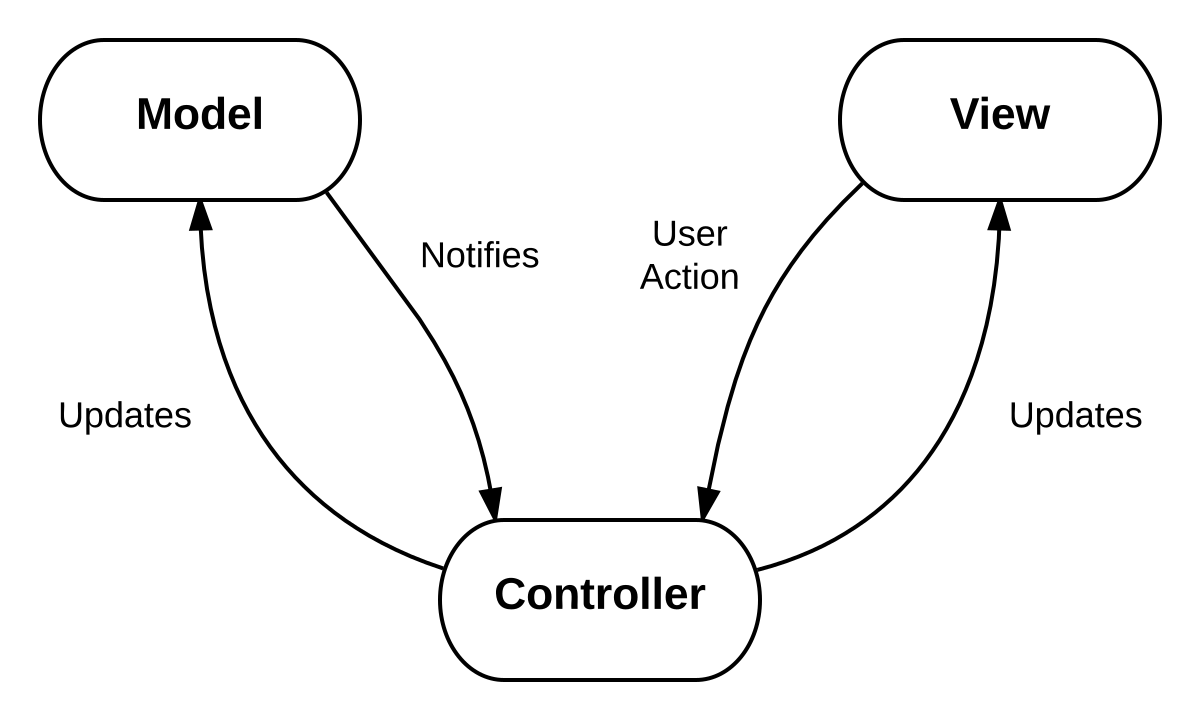
\includegraphics[width=10cm]{img/MVC.png}
  \captionof{figure}{Mô hình MVC}
\end{center}

Hệ thống được chia ra các thành phần riêng biệt với nhau nên trong quá trình kiểm thử sẽ dễ dàng phát hiện và chỉnh sửa lỗi. Bên cạnh đó, việc nâng cấp phần mềm cũng trở nên dễ dàng hơn

\section{Ứng dụng đa trang và ứng dụng đơn trang}
Khi phát triển một ứng dụng, có hai kiểu thiết kế phổ biến hiện nay là ứng dụng đa trang (Multi-page Application-MPA) và ứng dụng đơn trang (Single-page Application-SPA). Mỗi kiểu thiết kế có những ưu và nhược điểm riêng phù hợp với các ứng dụng khác nhau. Vì vậy để có thể phát triển ứng dụng một cách hiệu quả, nhà phát triển phải cân nhắc lựa chọn cách thiết kế phù hợp nhất với nhu cầu ứng dụng của mình.
\subsection{Ứng dụng đa trang (Multi-page Application-MPA)}
\textbf{Giới thiệu:}

Ứng dụng đa trang (MPA) là một web-app hay một website chứa nhiều trang liên kết và các trang con, được điều hướng bằng menu. Ứng dụng đa trang hoạt động theo kiểu "truyền thống", các thay đổi như hiển thị dữ liệu sẽ được thực hiện bằng cách hiển thị một trang mới trong trình duyệt.

Ứng dụng đa trang phù hợp với hầu hết các dự án. Hiện nay, ứng dụng đa trang được sử dụng rộng rãi trong nhiều lĩnh vực như thương mại điện tử (amazon.com), e-learning (lynda.com),...

\textbf{Ưu điểm:}
\begin{itemize}
    \item Cho phép khả năng mở rộng ứng dụng không giới hạn thông qua menu.
    \item Luồng điều hướng dễ dàng theo dõi. 
    \item Hỗ trợ tốt cho SEO, các ứng dụng đa trang dễ dàng phân cấp, sắp xếp các từ khoá cho từng trang, từng sản phẩm.
\end {itemize}

\textbf{Nhược điểm:}

\begin{itemize}
    \item Các ứng dụng đa trang có nhiều nội dung lớn thường tải chậm, ảnh hưởng đến trải nghiệm của người dùng.
    \item Khó thích nghi tốt với thiết bị di động.
\end {itemize}
\subsection{Ứng dụng đơn trang (Single-page Application-SPA):}
\textbf{Giới thiệu:}

Ứng dụng đơn trang (SPA) là một web-app hay một website tương tác với người dùng bằng cách tải lại một phần của trang hiện tại thay vì tải toàn bộ trang mới từ máy chủ. Cách hoạt động này hạn chế sự gián đoạn trải nghiệm của người dùng khi chuyển giữa các trang, giúp cho việc trải nghiệm ứng dụng gần giống với các desktop application.

Trong ứng dụng đơn trang, tất cả các tài nguyên cần thiết như mã HTML, JavaScript, CSS được tải duy nhất ở lần đầu tiên mở trang web. Các tài nguyên khác sẽ được tự động tải và thêm vào trang khi cần, thường là để đáp ứng hành động của người dùng. Ứng dụng SPA chỉ tải duy nhất một lần trong suốt quá trình sử dụng vì vậy giúp tiết kiệm băng thông cũng như giảm thời gian chờ đợi.

Ngày nay, ứng dụng đơn trang được sử dụng rộng rãi trên toàn thế giới, đặc biệt phù hợp các ứng dụng với lượng truy cập lớn, yêu cầu tốc độ cao như mạng xã hội, email, map. Một số ứng dụng sử dụng SPA nổi tiếng như Facebook, Instagram, Google Map, Gmail,...

\textbf{Ưu điểm:}
\begin{itemize}
    \item Tốc độ nhanh,
    \item Có khả năng làm việc với cache tốt, nên hiệu quả khi sử dụng ở chế độ offline.
    \item Thích nghi tốt với thiết bị di động.
\end{itemize}

\textbf{Nhược điểm:}

\begin {itemize}
    \item Không tối ưu hoá cho SEO tốt (các công cụ tìm kiếm). Việc tìm kiếm các nội dung trong ứng dụng đơn trang bằng các công cụ tìm kiếm (google.com, bing.com) thường ít hiệu quả.
    \item Khó khăn trong việc mở rộng.
\end {itemize}
\subsection{Kết luận và lựa chọn}
Nhận thấy hệ thống phòng tổ chức hành chính có những đặc điểm như sau:
\begin {itemize}
    \item Có nhiều nội dung tương đối giống nhau nên việc sử dụng ứng dụng đa trang là không cần thiết.
    \item Hệ thống tập trung vào tác vụ xử lý nên ưu tiên tốc độ cao.
    \item Hệ thống phát triển hỗ trợ hoạt động của phòng tổ chức hành chính do đó không cần quá chú trọng vào SEO.
\end {itemize}

Vì vậy nhóm quyết định sử dụng ứng dụng đơn trang vào ứng dụng phòng tổ chức hành chính.





\section{Các công nghệ front-end style}
\subsection{jQuery}
\begin{center}
  \captionsetup{type=figure}
  
\includegraphics[width=8cm]{img/jquery-logo.jpg}
  \captionof{figure}{jQuery}
\end{center}

jQuery là một thư viện Javascript nhanh, nhỏ và giàu tính năng. Nó làm cho mọi thứ như chuyển đổi và thao tác đối với HTML, xử lý sự kiện, hiệu ứng và Ajax đơn giản hơn nhiều với API dễ sử dụng, hoạt động trên vô số trình duyệt. Với sự kết hợp giữa tính linh hoạt và khả năng mở rộng, jQuery đã thay đổi cách hàng triệu người viết Javascript.\\

\textbf{Đặc điểm và thế mạnh:}
\begin{itemize}
    \item \textbf{Dễ sử dụng:} Đây là lợi thế chính khi sử dụng jquery, nó dễ dàng hơn so với nhiều thư viện Javascript chuẩn khác bởi cú pháp đơn giản và bạn chỉ phải viết ít dòng lệnh để tạo ra các chức năng tương tự. Chỉ với 10 dòng lệnh JQuery bạn có thể thay thế cả 20 chục dòng lệnh DOM JavaScript, tiết kiệm thời gian của người lập trình.
    \item \textbf{Là một thư viện lớn của Javascript:} Thực thi được nhiều chức năng hơn so với các thư viện Javascript khác
    \item \textbf{Cộng đồng mã nguồn mở mạnh mẽ:} JQuery đang còn tương đối mới, có một cộng đồng dành thời gian của họ để phát triển các plugin của JQuery. Như vậy có hàng trăm plugin được viết trước đó có sẵn để tải về ngay lập tức để đẩy nhanh quá trình viết code của bạn. Một lợi thế khác đằng sau này là hiệu quả và an toàn của các script.
    \item \textbf{Có nhiều tài liệu và hướng dẫn chi tiết:} Các trang web JQuery có một toàn bộ tài liệu
    \item \textbf{Hỗ trợ Ajax:} JQuery cho phép bạn phát triển các Ajax một cách dễ dàng. Ajax cho phép một giao diện kiểu dáng đẹp trên trang web, các chức năng có thể được thực hiện trên các trang mà không đòi hỏi toàn bộ trang được tải lại.
\end{itemize}
\subsection{Bootstrap}
\begin{center}
  \captionsetup{type=figure}
  
\includegraphics[width=5cm]{img/bootstrap-logo.png}
  \captionof{figure}{Bootstrap}
\end{center}

Bootstrap là một nền tảng (framework) miễn phí, mã nguồn mở, dựa trên HTML, CSS \& Javascript, nó được tạo ra để xây dựng các giao diện website tương thích với tất cả các thiết bị có kích thước màn hình khác nhau.
Hiện nay Bootstrap là một trong những framework được sử dụng nhiều nhất trên thế giới để tạo ra các Responsive Website. Bootstrap đã tạo ra một tiêu chuẩn riêng, và rất được các lập trình viên ưu chuộng.\\

\textbf{Đặc điểm và thế mạnh:}
\begin{itemize}
    \item Dễ sử dụng
    \item Tiết kiệm thời gian cho người dùng khi cần tạo ra các trang web tương thích với các thiết bị khác nhau
    \item Tương thích với các trình duyệt
\end{itemize}

\subsection{LESS}
\begin{center}
  \captionsetup{type=figure}
  \includesvg[width=6cm]{img/less-logo}
  \captionof{figure}{LESS}
\end{center}

LESS giúp viết đoạn mã CSS đơn giản, ngắn gọn và hiệu quả hơn, đồng thời cũng dễ quản lý hơn bằng cách thêm vào CSS các thành phần động như biến, mixins, toán tử và hàm. LESS được phát triển bởi một lập trình viên người Đức là Alexis Sellier. Các thành phần cơ bản của LESS:
\begin{itemize}
    \item Biến: được khai báo và gán cho các giá trị của thuộc tính
    \begin{verbatim}
        @width: 10px;
        @height: @width + 10px;

        #header {
          width: @width;
          height: @height;
        }
    \end{verbatim}
    \item Mixins cho phép gán toàn bộ thuộc tính của một class trong CSS và trong class khác bằng cách thêm tên class này như một thuộc tính của class kia. Nó gần giống với biến, nhưng thay giá trị bằng toàn bộ các thuộc tính của class. Mixins cũng có thể được dùng như hàm bằng cách truyền tham số.
    \begin{verbatim}
        .bordered {
            border-top: dotted 1px black;
            border-bottom: solid 2px black;
        }
        #menu a {
            color: #111;
            .bordered();
        }
        
        .post a {
            color: red;
            .bordered();
        }
    \end{verbatim}
\end{itemize}
\subsection{SASS}
\begin{center}
  \captionsetup{type=figure}
  
\includegraphics[width=4cm]{img/sass-logo.png}
  \captionof{figure}{SASS}
\end{center}

SASS (Syntactically Awesome StyleSheets) là một mở rộng của CSS, nó cho phép bạn sử dụng biến (variables), quy tắc xếp chồng (nested rules), mixins, ..., và tất cả chúng đều hoàn toàn tương thích với cú pháp của CSS.

\textbf{Các đặc tính của SASS}
\begin{itemize}
    \item Hoàn toàn tương thích với CSS
    \item Cung cấp các tiện ích vô cùng mạnh mẽ
    \item Giúp tiết kiệm thời gian viết CSS
    \item Tổ chức các files một cách rõ ràng, giúp cho việc dễ dàng phát triển và bảo trì
\end{itemize}

\textbf{Các quy tắc sử dụng SASS}
\begin{description}
    \item 1. Quy tắc xếp chồng\\
    Trong Sass, chúng ta có thể xếp chồng các thuộc tính như margin, padding, border, text... để tránh những khai báo rườm rà, dài dòng:
    \begin{verbatim}
        div {
          text: {
              align: center;
              decoration: none;
              transform: uppercase;
          }
          margin: {
            left: 10px;
            right: 50px;
          }
        }
    \end{verbatim}
    \item 2. Cách sử dụng biến\\
    Biến bắt đầu bằng ký hiệu \$ và được thiết lập như các thuộc tính CSS. Ví dụ:
    \begin{verbatim}
        $width: 10px;
        $height: $width + 10px;

        #header {
          width: $width;
          height: $height;
        }
    \end{verbatim}
    \item 3. Sử dụng Mixins:\\
    Giống như Mixins trong LESS, Mixins giúp tái tạo lại các thuộc tính
    \begin{verbatim}
        @mixin bordered {
            border-top: dotted 1px black;
            border-bottom: solid 2px black;
        }
        #menu a {
            color: #111;
            @include bordered;
        }
        
        .post a {
            color: red;
            @include bordered;
        }
    \end{verbatim}
    \item 4. Sử dụng kế thừa:\\
    Tính năng kế thừa cho phép chúng ta chỉ định cho một thành phần nào đó thừa hưởng tất cả các thuộc tính của một vùng chọn nào đó bất kỳ mà bạn đã khai báo sẵn.
    \begin{verbatim}
        .danger {
            color: red;
        }
        .danger-bold {
            @extend .danger;
            font-weight: bold;
        }
    \end{verbatim}
\end{description}

\section{Các nền tảng Frontend}
Front-end của một ứng dụng được hiểu là phần tương tác trực tiếp với người dùng. Nhà phát triển sử dụng kết hợp các ngôn ngữ như HTML, CSS, Javascipt,... thiết kế nên giao diện để người dùng có thể xem và tương tác trực tiếp với ứng dụng.

Hiện nay, các ứng dụng có nội dung ngày càng lớn, yêu cầu về giao diện và trải nghiệm người dùng ngày càng cao, gây khó khăn khi phát triển. Vì vậy, các front-end framework và thư viện ra đời giúp tiết kiệm thời gian lập trình, tối ưu hoá và dễ dàng tạo ra các tương tác thân thiện với người dùng.

Tuy nhiên lại có rất nhiều front-end framework và thư viện khác nhau, với các tính năng và đặc điểm nổi bật riêng. Vì vậy, nhóm quyết định tìm hiểu các thư viện, framework phổ biến nhất để từ đó đưa ra sự lựa chọn phù hợp cho ứng dụng của mình.
\subsection{React}
\begin{center}
  \captionsetup{type=figure}
  
\includegraphics[width=4cm]{img/React_logo.png}
  \captionof{figure}{React}
\end{center}
%  https://skillcrush.com/2019/05/14/what-is-react-js/
React là một thư viện Javascipt mã nguồn mở, được sử dụng để xây dựng giao diện người dùng, được tạo ra bởi các nhà phát triển của Facebook.

React nổi lên với xu hướng ứng dụng đơn trang, đơn giản và dễ dàng phối hợp với những thư viện Javascript khác. Trong báo cáo khảo sát lập trình viên StackOverflow 2019, React đã vươn lên vị trí thứ 2 ở mục các web framework phổ biến nhất.

Ngoài việc cung cấp mã thư viện React có thể sử dụng lại (tiết kiệm thời gian phát triển và giảm khả năng xảy ra lỗi mã hóa), React còn đi kèm với hai tính năng chính làm tăng thêm sức hấp dẫn cho các nhà phát triển JavaScript:
\begin{itemize}
    \item JSX
    \item Virtual DOM
\end{itemize}

Nhưng trên hết, React JS là một dự án nguồn mở, có nghĩa là bất kỳ ai cũng có thể tải xuống và sửa đổi mã nguồn miễn phí. Điều này cũng có nghĩa là, bất kỳ chức năng UI cụ thể nào mà bạn mong muốn giải quyết với React JS, đều có thư viện React để đáp ứng nhu cầu của bạn. Kích thước thư viện React của bạn có thể tăng theo cấp số nhân với các tiện ích thư viện được quản lý bởi cộng đồng React, bao gồm từ các bộ sưu tập các tính năng UI cá nhân đến các mẫu React JS hoàn chỉnh để xây dựng UI từ đầu.

\textbf{JSX:}\\
Phần chính của bất kỳ trang web cơ bản nào là HTML. Trình duyệt web đọc các tài liệu này và hiển thị chúng trên máy tính, máy tính bảng hoặc điện thoại dưới dạng trang web. Trong quá trình này, các trình duyệt tạo ra một thứ gọi là Mô hình Đối tượng Tài liệu (Document Object Model - DOM). Sau đó, các nhà phát triển có thể thêm nội dung động vào các dự án của họ bằng cách sửa đổi DOM bằng các ngôn ngữ như JavaScript.

JSX (viết tắt của JavaScript eXtension) là một phần mở rộng của React giúp các nhà phát triển web dễ dàng sửa đổi DOM của họ bằng cách sử dụng mã kiểu HTML đơn giản. Và kể từ khi hỗ trợ trình duyệt React JS mở rộng cho tất cả các trình duyệt web hiện đại, thì JS JSX tương thích với mọi nền tảng trình duyệt mà ta có thể đang làm việc.

\textbf{Virtual DOM:}\\
Trong trường hợp không sử dụng React JS (và JSX), trang web sẽ sử dụng HTML để cập nhật DOM của nó (quá trình khiến mọi thứ thay đổi trên màn hình mà không cần người dùng phải tự làm mới trang). Điều này hoạt động tốt đối với các trang web đơn giản, tĩnh, nhưng đối với các trang web động có sự tương tác của người dùng nặng thì nó có thể trở thành một vấn đề (vì toàn bộ DOM cần tải lại mỗi khi người dùng nhấp vào tính năng gọi để làm mới trang).

Tuy nhiên, nếu nhà phát triển sử dụng JSX để thao tác và cập nhật DOM của nó, React JS sẽ tạo ra thứ gọi là Virtual DOM. Virtual DOM (DOM ảo) là một bản sao của DOM, và React JS sử dụng bản sao này để xem những phần nào của DOM thực tế cần thay đổi khi xảy ra sự kiện (như người dùng nhấp vào nút).

Giả sử rằng một người dùng nhập một bình luận cho một bài đăng trên blog và nhấn nút Bình luận trực tuyến. Nếu không sử dụng React JS, toàn bộ DOM sẽ phải cập nhật để phản ánh sự thay đổi này (sử dụng thời gian và sức mạnh xử lý để thực hiện cập nhật này). Mặt khác, React quét Virtual DOM để xem những gì đã thay đổi sau hành động của người dùng (trong trường hợp này là một bình luận được thêm vào) và chỉ cập nhật có chọn lọc phần đó của DOM.

Kiểu cập nhật có chọn lọc này tốn ít sức mạnh tính toán hơn và thời gian tải ít hơn, nghe có vẻ không tiết kiệm được nhiều khi ta nói về một bình luận blog, nhưng khi nói về một trang web tất cả đều động và cập nhật gắn với thậm chí là trang web hơi phức tạp hơn thì ta sẽ nhận ra rằng nó tiết kiệm hơn rất nhiều.

\textbf{Đặc điểm và thế mạnh:}
\begin {itemize}
\item Được sử dụng để xây dựng ứng dụng đơn trang.
\item React cho phép các nhà phát triển tạo ra các ứng dụng web lớn có thể thay đổi dữ liệu mà không cần tải lại trang.
\item React hỗ trợ việc xây dựng những thành phần (components) giao diện người dùng có tính tương tác cao, có trạng thái và có thể tái sử dụng.
\item React không chỉ hoạt động trên phía người dùng, mà còn được sinh ra trên server và có thể kết nối với nhau.
\end {itemize}

\subsection{AngularJS \& Angular}
\begin{center}
  \captionsetup{type=figure}
  
\includegraphics[width=6cm]{img/angular-logo.png}
  \captionof{figure}{Angular}
\end{center}
\textbf{AngularJS}

AngularJS hay Angular 1 là một trong những công nghệ Javascript phổ biến nhất trong giới phát triển front-end. Nó được hậu thuẫn bởi Google và một cộng đồng lớn. AngularJS được tạo ra để xây dựng các ứng dụng web động (dynamic web app), và thường được sử dụng để tạo ra các ứng dụng đơn trang (Single Page Application - SPA).

Phiên bản AngularJS được phát triển dựa trên Javascipt nên dễ tiếp cận và được sử dụng rộng rãi. Tuy nhiên về mặt hiệu năng thì AngularJS không được đánh giá cao, thường bị đem ra so sánh với React. Hiện nay, những công ty phát triển phần mềm thường không chọn AngularJS để phát triển một sản phẩm mới.

Những vẫn đề mà Angular có thể giải quyết:
\begin{itemize}
    \item \textbf{Đăng ký callbacks:} Đăng ký hàm gọi lại làm phức tạp code. Loại bỏ mã soạn sẵn phổ biến như gọi lại là một điều tốt. Nó giúp giảm đáng kể số lượng mã hóa JavaScript mà bạn phải thực hiện và giúp dễ dàng xem ứng dụng của bạn làm gì.
    \item \textbf{Thao tác với HTML DOM bằng lập trình:} Thao tác HTML DOM là nền tảng của các ứng dụng AJAX, nhưng nó cồng kềnh và dễ bị lỗi. Bằng cách mô tả khai báo giao diện người dùng sẽ thay đổi như thế nào khi trạng thái ứng dụng của bạn thay đổi, ta sẽ thoát khỏi các tác vụ thao tác DOM cấp thấp. Hầu hết các ứng dụng được viết bằng AngularJS không bao giờ phải thao tác lập trình DOM, mặc dù vẫn có thể thao tác nếu muốn.
    \item \textbf{Sắp xếp dữ liệu và dữ liệu giao diện người dùng:} Các hoạt động CRUD chiếm phần lớn các nhiệm vụ của ứng dụng AJAX. Luồng dữ liệu sắp xếp theo thứ tự từ máy chủ sang đối tượng bên trong sang dạng HTML, cho phép người dùng sửa đổi biểu mẫu, xác thực biểu mẫu, hiển thị lỗi xác thực, quay lại mô hình bên trong và sau đó quay lại máy chủ, tạo ra rất nhiều bản tóm tắt code. AngularJS loại bỏ gần như tất cả các mẫu soạn sẵn này, để lại mã mô tả dòng chảy chung của ứng dụng thay vì tất cả các chi tiết triển khai.
    \item \textbf{Viết hàng tấn mã khởi tạo chỉ để bắt đầu:} Thông thường, ta cần phải viết rất nhiều khai báo khởi tạo chỉ để ứng dụng AJAX cơ bản như "Hello World" hoạt động. Với AngularJS, bạn có thể tự khởi động ứng dụng của mình một cách dễ dàng bằng các dịch vụ, được tự động đưa vào ứng dụng của bạn theo kiểu tiêm phụ thuộc giống như Guice. Điều này cho phép bạn bắt đầu phát triển các tính năng một cách nhanh chóng. Như một phần thêm vào, bạn có toàn quyền kiểm soát quá trình khởi tạo trong các trình kiểm tra tự động.
\end{itemize}

\textbf{Angular JS và Angular:}

Các phiên bản tiếp theo của Angular 2, 4, 5, 6, 7, 8 có tên chính thức là Angular, ra đời với nhiều sự khác biệt và cải tiến so với AngularJS:
\begin {itemize}
\item TypeScript thay cho JavaScript làm ngôn ngữ mặc định
\item Kiến trúc component-based
\item Cải thiện hiệu năng trên nền tảng web và mobile
\end {itemize}
Vì Angular 2 được viết lại từ đầu nên khác biệt hoàn toàn so với AngularJS nên việc nâng cấp từ AngulaJS lên Angular 2 khá khó khăn. Hiện nay cộng đồng lập trình viên vẫn đang sử dụng cả hai framework.

\textbf{Angular:}

Thế mạnh của Angular:
\begin{itemize}
    \item \textbf{Angular trình bày cho bạn không chỉ các công cụ mà còn thiết kế các mẫu để xây dựng dự án của bạn một cách dễ duy trì.} Khi một ứng dụng Angular được tạo ra đúng cách, ta sẽ không gặp phải một mớ các lớp và phương thức khó sửa đổi và thậm chí khó kiểm tra hơn. Code được cấu trúc thuận tiện và không cần phải mất nhiều thời gian để hiểu những gì đang diễn ra.
    \item \textbf{Nó là JavaScript, nhưng tốt hơn.} Angular được xây dựng với TypeScript, lần lượt dựa vào JS ES6. Ta không cần học một ngôn ngữ hoàn toàn mới, nhưng ta vẫn nhận được các tính năng tốt hơn.
    \item \textbf{Không cần phải tạo lại bicycle.} Với Angular, ta đã có rất nhiều công cụ để bắt đầu tạo ứng dụng ngay lập tức. Ta có các chỉ thị để cung cấp cho các phần tử HTML hành vi động. Ta có thể tăng sức mạnh cho các biểu mẫu bằng FormControl và giới thiệu các quy tắc xác thực khác nhau. Ta có thể dễ dàng gửi các yêu cầu HTTP không đồng bộ thuộc nhiều loại khác nhau. Ta có thể thiết lập định tuyến với ít rắc rối. Và còn nhiều điều tiện ích nữa mà Angular có thể cung cấp!
    \item \textbf{Các thành phần được tách rời.} Angular cố gắng để loại bỏ khớp nối chặt chẽ giữa các thành phần khác nhau của ứng dụng. Injection xảy ra theo kiểu NodeJS và ta có thể dễ dàng thay thế các thành phần khác nhau.
    \item \textbf{Tất cả các thao tác DOM diễn ra ở nơi nó nên diễn ra.} Với Angular, ta không kết hợp chặt chẽ việc trình bày và luận lí của ứng dụng làm cho việc đánh dấu của ta đơn giản và đơn giản hơn nhiều.
    \item \textbf{Kiểm thử là chủ yếu.} Angular có nghĩa là được kiểm thử kỹ lưỡng và nó hỗ trợ cả kiểm thử đơn vị và đầu cuối với các công cụ như Jasmine và Protractor.
    \item \textbf{Angular tương thích cho cả điện thoại va máy tính,} có nghĩa là ta có một framework cho nhiều nền tảng.
    \item \textbf{Angular được bảo trì tốt} và có một cộng đồng lớn và hệ sinh thái. Bạn có thể tìm thấy nhiều tài liệu trên framework này cũng như nhiều công cụ của bên thứ ba cũng tương đối hữu ích.
\end{itemize}

Như vậy, có thể nói Angular không chỉ là một framework, mà là một nền tảng trao quyền cho các nhà phát triển để xây dựng các ứng dụng cho web, di động và máy tính.

\subsection{VueJS}
\begin{center}
  \captionsetup{type=figure}
  
\includegraphics[width=4cm]{img/Vue-logo.png}
  \captionof{figure}{VueJS}
\end{center}

Vue.js gọi tắt là Vue, là một framework linh động (nguyên bản tiếng Anh: progressive framework) dùng để xây dựng giao diện người dùng (user interfaces). Khác với các framework nguyên khối (monolithic), Vue được thiết kế từ đầu theo hướng cho phép và khuyến khích việc phát triển ứng dụng theo từng bước. Khi phát triển lớp giao diện (view layer), người dùng chỉ cần dùng thư viện lõi (core library) của Vue, vốn rất dễ học và tích hợp với các thư viện hoặc dự án có sẵn. Cùng lúc đó, nếu kết hợp với những kĩ thuật hiện đại như SFC (single file components) và các thư viện hỗ trợ, Vue cũng đáp ứng được dễ dàng nhu cầu xây dựng những ứng dụng đơn trang với độ phức tạp cao hơn nhiều.

Vue có nhiều điểm tương đồng với React với Virtual DOM và các component có thể tái sử dụng. Vue.js cũng hỗ trợ tích hợp những thư viện khác vào framework mà không cần tốn quá nhiều công sức.
\subsection{Backbone.js}
\begin{center}
  \captionsetup{type=figure}
  
\includegraphics[width=8cm]{img/backbone.png}
  \captionof{figure}{Backbone}
\end{center}

Backbone là một thư viện Javascript, phục vụ cho việc phát triển front-end. Backbone sử dụng các component Event, Model, Collection, View, Router để tạo nên ứng dụng web. Backbone được các lập trình viên dùng nhiều bởi nó dễ sử dụng và áp dụng cho các ứng dụng Javascript.

Backbone đơn giản, gọn nhẹ và có thể kết hợp cùng các thư viện khác. Các ứng dụng thực tế sử dụng Backbone như LinkedIn Mobile, Foursquare, Basecamp,...

Backbone không có controller nên model và view được đồng bộ rất tốt. Tuy nhiên, việc không có controller đôi khi có thể gây ra hiện tượng nhập nhằn vì các thao tác làm trong controler giờ được trải rải rác vào model và view.
\subsection{Ember.js}
\begin{center}
  \captionsetup{type=figure}
  
\includegraphics[width=4cm]{img/ember-logo.png}
  \captionof{figure}{Ember.js}
\end{center}

Ember là một front-end framework Javascript mã nguồn mở vận hành trên mô hình Model-View-Viewmodel (MVVM). Ember cho phép phát triển tạo ra các ứng dụng đơn trang có thể mở rộng bằng cách kết hợp các thành ngữ phổ biến và các thực tiễn tốt nhất vào khung.
\subsection{Kết luận và lựa chọn}
Hiện nay có rất nhiều thư viện và frame-work hỗ trợ việc xây dựng giao diện, sau khi tìm hiểu nhóm quyết định lựa chọn ReactJs là công cụ phát triển chính dựa vào những đặc điểm nổi bật sau:
\begin{itemize}
    \item React xây dựng các ứng dụng đơn trang với hiệu suất cao, đã được kiểm chứng như Facebook, Instagram.
    \item React là công nghệ mã nguồn mở, có nhiều thư viện và các công cụ hỗ trợ xây dựng ứng dụng bằng React như Flux, Redux,...
    \item Hiện nay React đang được Facebook hỗ trợ và có cộng đồng sử dụng lớn, vì vậy React là một công nghệ đáng tin cậy và được cập nhập liên tục.
    \item Việc xây dựng ứng dụng di động trở nên dễ dàng hơn với React Native - mobile-framwork của Facebook được xây dựng dựa trên React.
\end {itemize}    
\section{Các thư viện cho ReactJs}

\subsection{Flux}
\begin{center}
  \captionsetup{type=figure}
  \includesvg[width=6cm]{img/flux-logo}
  \captionof{figure}{Flux}
\end{center}
\textbf{Giới thiệu:}

Flux là một kiến trúc phát triển ứng dụng mà Facebook sử dụng để hỗ trợ React. Flux giúp làm việc với các components của React một cách dễ dàng bằng cách sử dụng luồng dữ liệu một chiều (Unidirectional Data Flow). Giải pháp này khiến luồng dữ liệu trong ứng dụng luôn di chuyển theo 1 hướng duy nhất. Khi dữ liệu thay đổi, luồng này lại khởi chạy lại từ đầu.
\begin{center}
  \captionsetup{type=figure}
  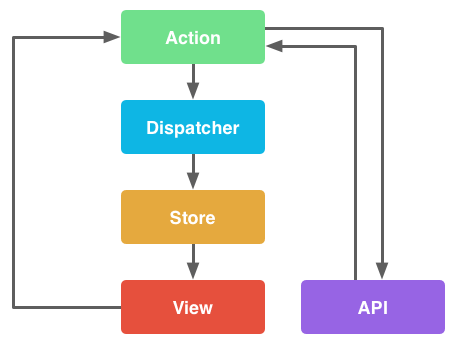
\includegraphics[width=14cm]{img/flux-flow}
  \captionof{figure}{Flux flow}
\end{center}

\textbf{Mô hình hoạt động của Flux:}
\begin{itemize}
    \item \textbf{View}: có nhiệm vụ hiển thị nội dung của ứng dụng (có thể hiểu giống như thành phần V trong mô hình MVC).
    
    Khi người dùng tương tác với ứng dụng làm thay đổi trạng thái (state) của ứng dụng (VD: thêm, sửa, xóa dữ liệu cá nhân), View sẽ thông qua Action gửi các thông tin thay đổi tới Dispatcher gồm có :
    \begin{itemize}
        \item action\_name: tên của Action (VD: ADD\_ITEM - thêm sản phẩm vào giỏ hàng).
        \item action\_payload: thông tin chi tiết nội dung muốn gửi (VD: Object chứa thông tin ID, quantity, price, ... của sản phẩm).
    \end{itemize}
    \item \textbf{Action}: Phát tán (dispatch) actions bằng Dispatcher đến những nơi đã đăng kí (register) nhận action đó.
    \item \textbf{Dispatcher}: Đối tượng trung gian, sau khi nhận được thông tin từ Action, Dispatcher làm nhiệm vụ truyền tải (broadcast) nội dung nhận được tới các Store đăng ký lắng nghe sự kiện thay đổi từ trước đó.
    \item \textbf{Store}: Trung tâm dữ liệu, sau khi nhận thông tin, Store tiến hành cập nhật dữ liệu (có thể hiểu việc cập nhật dữ liệu ở đây giống việc cập nhật state của Component). Sau khi cập nhật, Store bắn sự kiện xuống View để tiến hành cập nhật hiển thị cho người dùng.
    \item Ngoài ra trong sơ đồ trên còn có một thành phần API để lấy dữ liệu từ Remote Server.
\end {itemize}
Sơ đồ trên đảm bảo luồng dữ liệu di chuyển trong Flux bắt buộc đi theo một đường nhất định.

\subsection{Redux}
\begin{center}
  \captionsetup{type=figure}
  
\includegraphics[width=10cm]{img/redux-logo.png}
  \captionof{figure}{Redux}
\end{center}
\textbf{Giới thiệu:}
Do yêu cầu cho các ứng dụng single-page sử dụng Javascript ngày càng trở lên phức tạp thì code của chúng ta phải quản lý nhiều state hơn. Redux ra đời là một công cụ hỗ trợ cho các ứng dụng JavaScipt, giúp quản lý các trạng thái một cách khoa học và hiệu quả hơn.

Redux học hỏi kiến trúc của Flux nhưng nó lược bỏ đi sự phức tạp không cần thiết.
\begin{itemize}
    \item Redux không có khái niệm DISPATCHER.
    \item Redux chỉ có một STORE duy nhất thay vi nhiều STORE như của Flux.
    \item Các đối tượng Action sẽ được tiếp nhận và xử lý trực tiếp bởi STORE.
\end {itemize}
\textbf{Mô hình hoạt động của Flux:}
\begin{center}
  \captionsetup{type=figure}
  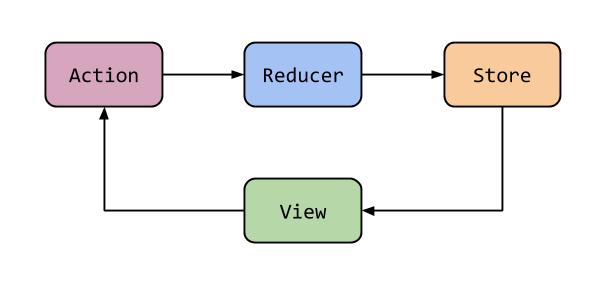
\includegraphics[width=10cm]{img/redux-architecture.png}
  \captionof{figure}{Redux architecture}
\end{center}
\begin{itemize}
    \item \textbf{Store}: Chứa state cho toàn bộ ứng dụng của bạn.
    \item \textbf{Reducers}: Lắng nghe các hành động (Actions) và thực hiện các thay đổi trên các giá trị của Store. Nó không thể biến đổi dữ liệu trên Store, nhưng phải trả lại một bộ dữ liệu mới (new data).
    \item \textbf{Actions}: Nó được định nghĩa như các khối thông tin (payloads) gửi dữ liệu từ ứng dụng của bạn đến Store. Chúng là nguồn thông tin duy nhất cho Store. Bạn có thể gửi chúng đến Store bằng cách sử dụng store.dispatch().
\end {itemize}
\subsection{Kết luận và lựa chọn}
Flux và Redux là hai công cụ hỗ trợ React được sử dụng phổ biến hiện nay. Tuy nhiên việc Redux ra đời sau và lấy cảm hứng từ kiến trúc Flux. Vì vậy, Redux mang nhiều ưu điểm được cải tiến từ Flux. Vậy nên khi sử dụng Redux sẽ đơn giản và ít gặp một số vấn đề khó giải quyết như khi sử dụng Flux.
Vì vậy nhóm quyết định sử dụng React kết hợp với Redux trong ứng dụng Phòng tổ chức hành chính.
\section{Công nghệ cho Server}
\subsection{Java}
\subsubsection{Java là gì}
\begin{center}
  \captionsetup{type=figure}
  \includesvg[width=4cm]{img/java.svg}
  \captionof{figure}{Java}
\end{center}

Java là một ngôn ngữ lập trình hướng đối tượng (OOP) và dựa trên các lớp (class). Khác với phần lớn ngôn ngữ lập trình thông thường, thay vì biên dịch mã nguồn thành mã máy hoặc thông dịch mã nguồn khi chạy, Java được thiết kế để biên dịch mã nguồn thành bytecode, bytecode sau đó sẽ được môi trường thực thi (runtime environment) chạy.

Trước đây, Java chạy chậm hơn những ngôn ngữ dịch thẳng ra mã máy như C và C++, nhưng sau này nhờ công nghệ "biên dịch tại chỗ" - Just in time compilation, khoảng cách này đã được thu hẹp, và trong một số trường hợp đặc biệt Java có thể chạy nhanh hơn. Java chạy nhanh hơn những ngôn ngữ thông dịch như Python, Perl, PHP gấp nhiều lần. Java chạy tương đương so với C\#, một ngôn ngữ khá tương đồng về mặt cú pháp và quá trình dịch/chạy.

Cú pháp Java được vay mượn nhiều từ C và C++ nhưng có cú pháp hướng đối tượng đơn giản hơn và ít tính năng xử lý cấp thấp hơn. Do đó việc viết một chương trình bằng Java dễ hơn, đơn giản hơn, đỡ tốn công sửa lỗi hơn. Nhưng về lập trình hướng đối tượng thì Java phức tạp hơn.

Trong Java, hiện tượng rò rỉ bộ nhớ hầu như không xảy ra do bộ nhớ được quản lý bởi Java Virtual Machine (JVM) bằng cách tự động "dọn dẹp rác". Người lập trình không phải quan tâm đến việc cấp phát và xóa bộ nhớ như C, C++. Tuy nhiên khi sử dụng những tài nguyên mạng, file IO, database (nằm ngoài kiểm soát của JVM) mà người lập trình không đóng (close) các streams thì rò rỉ dữ liệu vẫn có thể xảy ra.

\subsubsection{Đặc điểm của java}

Java có những đặc điểm cơ bản như sau:
\begin{itemize}
    \item \textbf{Hướng đối tượng:} Trong Java, mọi thứ đều là Object. Java có thể mở rộng vì nó dựa trên mô hình Object.
    \item \textbf{Nền tảng độc lập:} Không giống như nhiều ngôn ngữ lập trình khác (C, C++), khi Java được biên dịch, nó không biên dịch sang một máy tính cụ thể trên nền tảng nào, thay vào đó là những byte code độc lập với nền tảng. Byte code này được phân phối trên web và được thông dịch bằng Virtual Machine (JVM) trên bất cứ nền tảng nào mà nó đang chạy.
    \item \textbf{Đơn giản:} Java được thiết kế để dễ học. Nếu bạn hiểu cơ bản về khái niệm lập trình hướng đối tượng Java, thì có thể nắm bắt ngôn ngữ này rất nhanh.
    \item \textbf{Bảo mật:} Với tính năng an toàn của Java, nó cho phép phát triển những hệ thống không có virus, giả mạo. Các kỹ thuật xác thực dựa trên mã hóa công khai.
    \item \textbf{Kiến trúc trung lập:} Trình biên dịch của Java tạo ra một định dạng file object có kiến trúc trung lập, làm cho code sau khi biên dịch có thể chạy trên nhiều bộ vi xử lý, với sự hiện diện của Java runtime system.
    \item \textbf{Portable:} Là kiến trúc trung lập và không phụ thuộc vào việc thực hiện là những đặc điểm chính nhất khi nói về khía cạnh Portable của Java. Trình biên dịch trong Java được viết bằng ANSI C với một ranh giới portable gọn gàng, đó là một subset POSIX (giao diện hệ điều hành linh động). Bạn có thể mang byte code của Java lên bất cứ nền tảng nào.
    \item \textbf{Mạnh mẽ:} Java nỗ lực loại trừ những tình huống dễ bị lỗi bằng cách nhấn mạnh chủ yếu là kiểm tra lỗi thời gian biên dịch và kiểm tra runtime.
    \item \textbf{Đa luồng:} Với tính năng đa luồng của Java, bạn có thể viết các chương trình có thể thực hiện nhiều tác vụ đồng thời. Tính năng này cho phép các nhà phát triển xây dựng các ứng dụng tương tác có thể chạy trơn tru.
    \item \textbf{Thông dịch:} Byte code của Java được dịch trực tiếp tới các nền tảng gốc và nó không được lưu trữ ở bất cứ đâu. 
    \item \textbf{Hiệu suất cao:} Với việc sử dụng trình biên dịch Just-In-Time, Java cho phép thực thi với hiệu suất cao, nhanh chóng phát hiện, gỡ lỗi.
    \item \textbf{Phân tán:} Java được thiết kế cho môi trường phân tán của Internet.
    \item \textbf{Linh động:} Java được coi là năng động hơn C hay C++ vì nó được thiết kế để thích nghi với môi trường đang phát triển. Các chương trình Java có thể mang theo một lượng lớn thông tin run-time, được sử dụng để xác minh và giải quyết các truy cập đến đối tượng trong thời gian chạy.
\end{itemize}
\subsubsection{Java được dùng ở đâu?}

Ta có thể bắt gặp Java ở rất nhiều nơi, từ những trang web thương mại điện tử đến ứng dụng Android, từ ứng dụng khoa học đến ứng dụng tài chính như hệ thống giao dịch điện tử, trò chơi như Minecrafr đến các ứng dụng trên máy tính như Eclipse, Netbeans, IntelliJ,...
\begin{itemize}
    \item \textbf{Ứng dụng Android:} Nếu muốn nhìn thấy một sản phẩm được tạo ra từ Java thì thật đơn giản, hãy mở điện thoại Android lên và bất kỳ ứng dụng nào bạn nhìn thấy cũng chính là một sản phẩm như vậy, được viết bằng ngôn ngữ lập trình Java, với Android API của Google, tương tự như JDK. Với sự phát triển của Android ngày nay, hầu hết lập trình viên Java đều là những người viết app cho Android. Android sử dụng JVM và cách đóng gói khác nhau, nhưng code thì vẫn được viết bằng Java.
    \item \textbf{Các ứng dụng máy chủ dùng trong dịch vụ tài chính:} Trong ngành dịch vụ tài chính Java chiếm một vị trí khá lớn. Nhiều ngân hàng đầu tư toàn cầu như Goldman Sachs, Citigroup, Barclays, Standard Charted và các ngân hàng khác sử dụng Java để viết hệ thống giao dịch điện tử front office và back office, viết hệ thống giải quyết và xác nhận, dự án xử lý dữ liệu,... Java chủ yếu được sử dụng để viết ứng dụng cho máy chủ, không có front end, nhận dữ liệu từ một máy chủ khác, xử lý nó và gửi đến một tiến trình tiếp theo.
    \item \textbf{Ứng dụng Web:} Java cũng chiếm được một thị phần khá lớn trong lĩnh vực thương mại điện tử và ứng dụng web. Có rất nhiều dịch vụ RESTfull được tạo bằng cách sử dụng Spring MVC, Struts 2.0 và những framework tương tự. Thậm chí những ứng dụng web đơn giản như Servlet, JSP và Struts cũng rất phổ biến trong các dự án khác nhau của chính phủ. Nhiều cơ quan chính phủ, y tế, bảo hiểm, giáo dục, quốc phòng và những bộ phận khác có ứng dụng web được xây dựng bằng Java.
    \item \textbf{Công cụ phần mềm:} Nhiều phần mềm hữu ích và công cụ phát triển được viết và triển khai trong Java, ví dụ như Eclipse, InetelliJ Idea và Netbans IDE. Rất nhiều phần mềm trên máy tính để bàn cũng được viết bằng Java. 
    \item \textbf{Công nghệ Big Data:} Hadoop và các công nghệ dữ liệu lớn khác cũng đang sử dụng Java theo cách này hay cách khác. Apache của Java dựa trên HBase và Accumulo (mã nguồn mở), ElasticSearch cũng vậy. Tuy Java không phải kẻ thống trị trong lĩnh vực này, vì có những công nghệ như MongoDB được viết bằng C ++, nhưng Java có tiềm năng để đạt được thị phần ngày càng tăng nếu Hadoop hoặc ElasticSearch lớn mạnh.
    \item \textbf{Ứng dụng khoa học:} Java thường được lựa chọn mặc định cho các ứng dụng khoa học, bao gồm xử lý ngôn ngữ tự nhiên. Lý do chính là vì Java an toàn hơn, portable, duy trì và đi kèm với những công cụ cấp cao tương đương C++ hay những ngôn ngữ lập trình khác.
\end{itemize}

\subsubsection{Thế mạnh của Java}

Cũng như nhiều ngôn ngữ lập trình khác, trình duyệt Java cũng có cho mình khá nhiều ưu điểm. Trong đó cần được kể tới như: hướng đối tượng rộng, có một nền tảng riêng biệt, có thiết kế đơn giản, khả năng bảo mật cao, nhanh và mạnh.
\begin{itemize}
    \item \textbf{Hướng đối tượng rộng:} Hướng đối tượng rộng trong Java chính là tất cả những thứ đều được mở rộng, trong đó thì Java sẽ được dùng dựa trên các mô hình là Object.
    \item \textbf{Java có nền tảng riêng biệt:} Java có nền tảng riêng biệt, người ta nói như vậy là bởi khi nhận được một câu lệnh nào đó, thì Java sẽ tự động thực hiện biên tập câu lệnh đó sang những Bite Code ở dạng độc lập. Trong đó, Bite Code độc lập này sẽ được hỗ trợ bởi các dịch bằng Vitual Machile với bất cứ phần mềm, ứng dụng nào có sử dụng tới nó.
    \item \textbf{Thiết kế mẫu khá đơn giản:} Không giống như nhiều ngôn ngữ lập trình khác, Java có thiết kế mẫu khá là đơn giản bởi thế mà những nhà lập trình viên không cần phải mất quá nhiều thời gian theo học. Muốn học tốt, thành thạo về Java thì mỗi người chỉ mất từ 1 đến 3 năm là đã có thể thành công.
    \item \textbf{Tính bảo mật cao:} Tính bảo mật cao, chính là một ưu điểm của Java so với các trình duyệt khác. Trong đó, khả năng của Java là phát hiện được những thành phần có chứa các virut độc hại, rồi sau đó nó cũng có thể “tiêu diệt” được  virut đó. Để thực hiện được điều này, những nhà lập trình viên ra Java đã phát triển cho nó những thuật toán ở mức độ cao nhất.
    \item \textbf{Nhanh và mạnh:} Đối với ưu điểm này, Java là một trình duyệt có được khả năng xử lý những tình huống bị xảy ra trên máy chủ rất nhanh. Bên cạnh đó, nó cũng có được khả năng truyền dẫn về internet với tốc độ cao, không kém gì những ứng dụng khác.
\end{itemize}

\subsubsection{Framework Spring}
\begin{center}
  \captionsetup{type=figure}
  
\includegraphics[width=15cm]{img/spring.png}
  \captionof{figure}{Spring Java}
\end{center}

Spring là framework phát triển ứng dụng phổ biến nhất dành cho Java Enterprise. Ban đầu nó được viết bởi Rod Johnson và lần đầu tiên được phát hành theo giấy phép Apache 2.0 vào tháng 6 năm 2003. Spring có kích thước nhẹ, phiên bản cơ bản của Spring framework có kích thước khoảng 2MB.

Spring framework là một Java Platform mã nguồn mở, một giải pháp gọn nhẹ dành cho Java Enterprise. Với Spring Framework các nhà phát triển có thể tạo ra các mã có hiệu suất cao, dễ kiểm thử và có thể sử dụng lại được.

Các tính năng core của Spring Framework có thể được sử dụng trong việc phát triển bất kỳ ứng dụng Java nào. Bên cạnh đó, phần mở rộng được sử dụng để xây dựng các ứng dụng web trên nền tảng Java EE. Mục tiêu của Spring Framework là làm cho việc phát triển ứng dụng J2EE dễ dàng hơn và thúc đẩy việc lập trình tốt hơn bằng mô hình POJO-based.
\begin{center}
  \captionsetup{type=figure}
  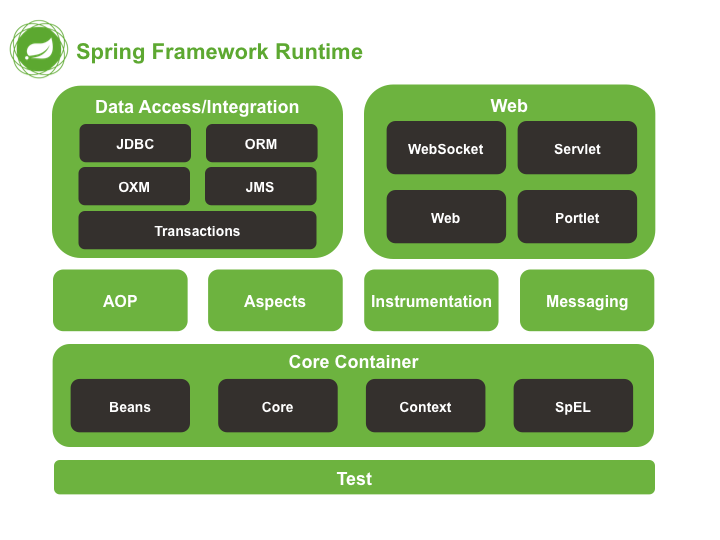
\includegraphics[width=15cm]{img/spring_runtime.png}
  \captionof{figure}{Spring Framework Runtime}
\end{center}

\subsubsection{Điểm mạnh của Framework Spring}

Dưới đây là danh sách các lợi ích tuyệt vời của việc sử dụng Spring Framework:
\begin{itemize}
    \item Spring cho phép các nhà phát triển tạo các ứng dụng cấp Enterprise sử dụng các POJO. Lợi ích của việc sử dụng các POJO là bạn không cần một sản phẩm chứa EJB như một máy chủ ứng dụng, mà bạn chỉ có thể sử dụng một bộ chứa servlet mạnh mẽ như Tomcat hoặc một số sản phẩm thương mại khác.
    \item Spring được tổ chức theo kiểu mô đun. Mặc dù số lượng các gói và các lớp là khá nhiều, nhưng bạn chỉ cần quan tâm đến những gì bạn cần và không cần quan tâm đến phần còn lại.
    \item Spring sử dụng một số công nghệ hiện có như một số ORM Framework, logging frameworks, JEE, Quartz, JDK timers và các công nghệ View khác.
    \item Dễ dàng để kiểm thử một chương trình được viết bằng Spring.
    \item Web framework của Spring là một Web MVC framework có thiết kế tốt, nó là một thay thế tuyệt vời cho Struts và các công nghệ kém phổ biến khác.
    \item Spring cung cấp một API thuận tiện để dịch các ngoại lệ công nghệ cụ thể (ném bởi JDBC, Hibernate, hoặc JDO chẳng hạn) vào các trường hợp ngoại lệ nhất quán, không được kiểm soát.
    \item IoC Container có trọng lượng nhẹ. Điều này có lợi cho việc phát triển và triển khai các ứng dụng trên các máy tính có bộ nhớ và tài nguyên CPU hạn chế.
    \item Spring cung cấp một giao diện quản lý transaction nhất quán có thể mở rộng đến một local transaction (ví dụ như sử dụng một cơ sở dữ liệu) và mở rộng lên các global transaction (sử dụng JTA).
\end{itemize}
\subsection{Python}
\subsubsection{Python là gì}

\begin{center}
  \captionsetup{type=figure}
  \includesvg[width=12cm]{img/python.svg}
  \captionof{figure}{Python}
\end{center}

Python là một ngôn ngữ thông dịch bậc cao, đa mục đích được tạo bởi Guido van Rossum vào năm 1991. Python được thiết kế với ưu điểm mạnh là dễ đọc, dễ học và dễ nhớ. Python là ngôn ngữ có hình thức rất sáng sủa, cấu trúc rõ ràng, thuận tiện cho người mới học lập trình. Cấu trúc của Python còn cho phép người sử dụng viết mã lệnh với số lần gõ phím tối thiểu.
\subsubsection{Đặc điểm của Python}
\begin{itemize}
    \item \textbf{Ngôn ngữ lập trình đơn giản, dễ học:} Python có cú pháp rất đơn giản, rõ ràng. Nó dễ đọc và viết hơn rất nhiều khi so sánh với những ngôn ngữ lập trình khác như C++, Java, C\#. Python làm cho việc lập trình trở nên thú vị, cho phép bạn tập trung vào những giải pháp chứ không phải cú pháp.
    \item \textbf{Miễn phí, mã nguồn mở:} Bạn có thể tự do sử dụng và phân phối Python, thậm chí là dùng cho mục đích thương mại. Vì là mã nguồn mở, bạn không những có thể sử dụng các phần mềm, chương trình được viết trong Python mà còn có thể thay đổi mã nguồn của nó. Python có một cộng đồng rộng lớn, không ngừng cải thiện nó mỗi lần cập nhật.
    \item \textbf{Khả năng di chuyển:} Các chương trình Python có thể di chuyển từ nền tảng này sang nền tảng khác và chạy nó mà không có bất kỳ thay đổi nào. Nó chạy liền mạch trên hầu hết tất cả các nền tảng như Windows, MacOS, Linux.
    \item \textbf{Khả năng mở rộng và có thể nhúng:} Giả sử một ứng dụng đòi hỏi sự phức tạp rất lớn, bạn có thể dễ dàng kết hợp các phần code bằng C, C++ và những ngôn ngữ khác (có thể gọi được từ C) vào code Python. Điều này sẽ cung cấp cho ứng dụng của bạn những tính năng tốt hơn cũng như khả năng scripting mà những ngôn ngữ lập trình khác khó có thể làm được.
    \item \textbf{Ngôn ngữ thông dịch cấp cao:} Không giống như C/C++, với Python, bạn không phải lo lắng những nhiệm vụ khó khăn như quản lý bộ nhớ, dọn dẹp những dữ liệu vô nghĩa,... Khi chạy code Python, nó sẽ tự động chuyển đổi code sang ngôn ngữ máy tính có thể hiểu. Bạn không cần lo lắng về bất kỳ hoạt động ở cấp thấp nào.
    \item \textbf{Thư viện tiêu chuẩn lớn để giải quyết những tác vụ phổ biến:} Python có một số lượng lớn thư viện tiêu chuẩn giúp cho công việc lập trình của bạn trở nên dễ thở hơn rất nhiều, đơn giản vì không phải tự viết tất cả code. Ví dụ: Bạn cần kết nối cơ sở dữ liệu MySQL trên Web server? Bạn có thể nhập thư viện MySQLdb và sử dụng nó. Những thư viện này được kiểm tra kỹ lưỡng và được sử dụng bởi hàng trăm người. Vì vậy, bạn có thể chắc chắn rằng nó sẽ không làm hỏng code hay ứng dụng của mình.
    \item \textbf{Hướng đối tượng:} Mọi thứ trong Python đều là hướng đối tượng. Lập trình hướng đối tượng (OOP) giúp giải quyết những vấn đề phức tạp một cách trực quan. Với OOP, bạn có thể phân chia những vấn đề phức tạp thành những tập nhỏ hơn bằng cách tạo ra các đối tượng.
\end{itemize}
\subsubsection{Python được dùng ở đâu?}
\begin{itemize}
    \item \textbf{Lập trình ứng dụng web:} Ta có thể tạo web app có khả năng mở rộng (scalable) được bằng cách sử dụng framework và CMS (Hệ thống quản trị nội dung) được tích hợp trong Python. Vài nền tảng phổ biến để tạo web app là:  Django, Flask, Pyramid, Plone, Django CMS. Các trang như Mozilla, Reddit, Instagram và PBS đều được viết bằng Python.
    \item \textbf{Khoa học và tính toán:} Có nhiều thư viện trong Python cho khoa học và tính toán số liệu, như SciPy và NumPy, được sử dụng cho những mục đích chung chung trong tính toán. Và, có những thư viện cụ thể như: EarthPy cho khoa học trái đất, AstroPy cho Thiên văn học,... Ngoài ra, Python còn được sử dụng nhiều trong machine learning, khai thác dữ liệu và deep learning.
    \item \textbf{Tạo nguyên mẫu phần mềm:} Python chậm hơn khi so sánh với các ngôn ngữ được biên dịch như C++ và Java. Nó có thể không phải là lựa chọn tốt nếu nguồn lực bị giới hạn và yêu cầu về hiệu quả là bắt buộc. Tuy nhiên, Python là ngôn ngữ tuyệt vời để tạo những nguyên mẫu (bản chạy thử - prototype). Ví dụ, bạn có thể sử dụng Pygame (thư viện viết game) để tạo nguyên mẫu game trước. Nếu thích nguyên mẫu đó có thể dùng C++ để viết game thực sự.
    \item \textbf{Ngôn ngữ tốt để dạy lập trình:} Python được nhiều công ty, trường học sử dụng để dạy lập trình cho trẻ em và những người mới lần đầu học lập trình. Bên cạnh những tính năng và khả năng tuyệt vời thì cú pháp đơn giản và dễ sử dụng của nó là lý do chính cho việc này.
\end{itemize}
\subsubsection{Thế mạnh của Python}
\begin{itemize}
  \item \textbf{Đơn giản:} Cú pháp đơn giản giúp cho người lập trình dễ dàng đọc và tìm hiểu.
  \item \textbf{Tốc độ:} Python có tốc độ xử lý nhanh hơn so với ngôn ngữ PHP.
  \item \textbf{Tương tác:} Chế độ tương tác cho phép người lập trình thử nghiệm tương tác sửa lỗi của các đoạn mã.
  \item \textbf{Chất lượng:} Thư viện có tiêu chuẩn cao, Python có khối cơ sở dữ liệu khá lớn nhằm cung cấp giao diện cho tất cả các CSDL thương mại lớn.
  \item \textbf{Thuận tiện:} Python được biên dịch và chạy trên tất cả các nền tảng lớn hiện nay.
  \item \textbf{Mở rộng:} Với tính năng này, Python cho phép người lập trình có thể thêm hoặc tùy chỉnh các công cụ nhằm tối đa hiệu quả có thể đạt được trong công việc.
\end{itemize}
\subsubsection{Framework Django}
\begin{center}
  \captionsetup{type=figure}
  
\includegraphics[width=12cm]{img/django.png}
  \captionof{figure}{Django}
\end{center}

Django là một web framework miễn phí mã nguồn mở được viết bằng Python. Django sử dụng mô hình Model-View-Control (MVC). Django được phát triển bởi Django Software Foundation(DSF) – một tổ chức phi lợi nhuận độc lập.

Mục tiêu chính của Django là đơn giản hóa việc tạo các website phức tạp có sử dụng cơ sở dữ liệu. Django tập trung vào tính năng “có thể tái sử dụng” và “có thể tự chạy” của các component, tính năng phát triển nhanh, không làm lại những gì đã làm. Một số website phổ biến được xây dựng từ Django là Pinterest, Instagram, Mozilla, và Bitbucket.

Django là một trong những framework phát triển web được yêu thích nhất cho việc phát triển các ứng dụng Python. Framework Django cho phép nguyên lý DRY (Don't Repeat Yourself) 

Không như các framework khácc, framework full-stack sử dụng miễn phí và mã nguồn mở của Python bao gồm một số lượng lớn các tính năng tích hợp thay vì cung cấp chúng dưới dạng các thư viện riêng lẻ. Django sử dụng ORM của nó để ánh xạ các đối tượng vào các bảng cơ sở dữ liệu. Điều này cho phép code hoạt động trên các cơ sở dữ liệu khác nhau cũng như giúp việc di chuyển từ cơ sở dữ liệu này sang cơ sở dữ liệu khác dễ dàng hơn. Mặc dù Django có hỗ trợ cho MySQL, PostgreSQL, SQLite và Oracle Database, nhưng nó vẫn có thể hỗ trợ các cơ sở dữ liệu khác thông qua trình điều khiển của bên thứ ba.

\textbf{Các điểm nổi bật chính:}
\begin{itemize}
    \item Học tập nhanh. Tương tự Python, Django cũng rất dễ học, không như Ruby on Rails.
    \item Tự động tạo SQL tables. Django sẽ thay bạn làm công việc này khi bạn đã xác định được cấu trúc.
    \item Tạo forms. Khi bạn đã tạo được Form class trong Django và linked đến model, form generator trong Django sẽ đảm nhận render form, xác minh và lưu trưc data.
    \item Admin Interface. Tương tự SQL table, khi bạn đã xác định được cấu trúc, Django sẽ tạo một admin interface cho phép bạn quản lý database (không khác gì PhpMyAdmin được build-in trong Django cả.)
    \item Django Shell. Python shell, ngay trong môi trường của Django project, chính là lợi thế mà Django shell mang lại. Tính năng này rất hữu hiệu khi debug (thường khó thực hiện trên PHP hơn).
\end{itemize}

\subsubsection{Framework Flask}
\begin{center}
  \captionsetup{type=figure}
  
\includegraphics[width=12cm]{img/flask.png}
  \captionof{figure}{Flask}
\end{center}

Flask là một web frameworks, nó thuộc loại micro-framework được xây dựng bằng ngôn ngữ lập trình Python. Flask cho phép bạn xây dựng các ứng dụng web từ đơn giản tới phức tạp. Nó có thể xây dựng các api nhỏ, ứng dụng web chẳng hạn như các trang web, blog, trang wiki hoặc một website dựa theo thời gian hay thậm chí là một trang web thương mại. Flask cung cấp cho bạn công cụ, các thư viện và các công nghệ hỗ trợ bạn làm những công việc trên.

Flask là một micro-framework. Điều này có nghĩa Flask là một môi trường độc lập, ít sử dụng các thư viện khác bên ngoài. Do vậy, Flask có ưu điểm là nhẹ, có rất ít lỗi do ít bị phụ thuộc cũng như dễ dàng phát hiện và xử lý các lỗi bảo mật.

\textbf{Tính năng của Framework Flask:}
\begin{itemize}
    \item Phát triển máy chủ.
    \item Phát triển trình gỡ lỗi.
    \item Hỗ trợ sẵn sàng để kiểm thử đơn vị.
    \item Jinja2 templates.
    \item RESTful request dispatch.
    \item Hỗ trợ bảo mật cookie.
    \item Full WSGI compliant.
    \item Tài liệu mở rộng.
    \item Dựa trên Unicode.
    \item Khả năng tương thích công cụ dựa trên ứng dụng Google.
    \item Nhiều tiện ích mở rộng cho các tính năng mong muốn.
    \item Tính modular và thiết kế gọn nhẹ.
    \item ORM-agnostic.
    \item Độ linh hoạt cao.
    \item Cung cấp xử lý HTTP request.
    \item API có độc đáo và mạch lạc.
    \item Dễ dàng triển khai.
\end{itemize}

\textbf{Điểm mạnh của Framework Flask:}
\begin{itemize}
  \item \textbf{Flask là một micro web framework:} Flask là một micro web framework được viết bằng Python, không yêu cầu tool hay thư viện cụ thể nào. “Micro” không có nghĩa là thiếu chức năng mà “micro” theo triết lý thiết kế là cung cấp một lõi chức năng “súc tích” nhất cho ứng dụng web nhưng người dùng có thể mở rộng bất cứ lúc nào. Flask luôn hỗ trợ các thành phần tiện ích mở rộng cho ứng dụng như tích hợp cơ sở dữ liệu, xác thực biểu mẫu, xử lý upload, các công nghệ xác thực, template, email, RESTful..., chỉ khác là khi nào bạn muốn thì bạn mới đưa vào thôi. Người dùng có thể tập trung xây dựng web application ngay từ đầu trong một khoảng thời gian rất ngắn và có thể phát triển quy mô của ứng dụng tùy theo yêu cầu.
  \item \textbf{Flask dễ cài đặt và triển khai:} Sau khi cài đặt Python, để cài đặt Flask chỉ cần bạn gõ lệnh: pip install Flask Bây giờ chúng ta thử tạo ứng dụng web với câu chào Hello World!. Thật đơn giản bạn sẽ tạo một folder với tên folder là tên ứng dụng, sau đó, tạo một tập tin .py và viết code. Flask tập trung vào sự tối giản, cho phép chúng ta xây dựng ứng dụng nhanh hơn.
  \item \textbf{Flask thật sự phù hợp cho việc xây dựng các web application có quy mô vừa và nhỏ, các API và web services:} 
  \begin{itemize}
    \item Xây dựng web application rất giống với việc viết các module Python chuẩn, cấu trúc gọn gàng và rõ ràng.
    \item Thay vì cung cấp hết tất cả mọi thứ, Flask cung cấp cho người dùng các thành phần cốt lõi thường được sử dụng nhất của khung ứng dụng web như URL routing, request and response object, template...
    \item Với Flask, việc chọn component nào cho ứng dụng là việc của chúng ta. Điều này thật tuyệt, vì mỗi web application có những đặc điểm và tính năng riêng, nó không phần phải chứa các component mà nó không dùng.
\end{itemize}
  \item \textbf{Flask giúp ta tập trung xây dựng ý tưởng, mục tiêu của riêng mình:} Flask có kiến trúc nhỏ, gọn nên bạn hoàn toàn không bị bó buộc bởi bộ khung cồng kềnh, không gặp bất cứ khó khăn nào khi cấu hình hay tổ chức ứng dụng. Không những thế, Flask còn có các ưu điểm nổi bật như: cực kỳ linh hoạt, tối giản, dễ tìm hiểu và sử dụng, định tuyến dễ dàng, rất dễ mở rộng. Vì vậy, công việc chính của ta là chỉ cần xác định ý tưởng, mục tiêu, tập trung vào việc xây dựng ứng dụng web mà thôi.
  \item \textbf{Nguồn tài liệu tham khảo về Flask rất phong phú:} Flask cung cấp rất nhiều tài liệu từ cài đặt đến thực hiện và triển khai, từ hướng dẫn nhanh đến hướng dẫn chi tiết. Ta có thể dễ dàng tìm kiếm, tham khảo, học tập về lập trình web application với Flask framework miễn phí trên Internet.
  \item \textbf{Cộng đồng Flask khá lớn:} Ta có thể dễ dàng, nhanh chóng tìm được giải pháp từ cộng đồng người sử dụng Flask mỗi khi gặp vấn đề cần giúp đỡ ví dụ như gặp lỗi, cách cài đặt thư viện, cách triển khai ứng dụng.
  \item \textbf{Mức độ phổ biến:} Có nhiều khách hàng đặt web application được xây dựng từ Flask Framework như Pinterest, LinkedIn, Twilio, Reddit, Netflix, Uber…
\end{itemize}
\subsection{NodeJS}
\subsubsection{NodeJS là gì}

\begin{center}
  \captionsetup{type=figure}
  \includesvg[width=10cm]{img/nodejs.svg}
  \captionof{figure}{NodeJS}
\end{center}


NodeJS là một mã nguồn được xây dựng dựa trên nền tảng Javascript V8 Engine, nó được sử dụng để xây dựng các ứng dụng web như các trang video clip, các forum và đặc biệt là trang mạng xã hội phạm vi hẹp. NodeJS là một mã nguồn mở được sử dụng rộng bởi hàng ngàn lập trình viên trên toàn thế giới. NodeJS có thể chạy trên nhiều nền tảng hệ điều hành khác nhau từ Windows cho tới Linux, OSX nên đó cũng là một lợi thế. NodeJS cung cấp các thư viện phong phú ở dạng Javascript module khác nhau giúp đơn giản hóa việc lập trình và giảm thời gian ở mức thấp nhất.

\subsubsection{Đặc điểm của NodeJS}

\begin{itemize}
  \item \textbf{Realtime:} Đây là tính năng quan trọng nhất của NodeJS. Realtime ở đây chính là xử lý giao tiếp từ client tới máy chủ theo thời gian thực. Giống như khi bạn lướt Facebook thì mỗi khi bạn comment hay like một topic nào đó thì ngay lập tức chủ topic và những người đã comment trên đó sẽ nhận được thông báo là bạn đã comment.
  \item \textbf{Không đồng bộ:} Tất cả các API của NodeJS đều không đồng bộ (none-blocking), nó chủ yếu dựa trên nền của NodeJS Server và chờ đợi Server trả dữ liệu về. Việc di chuyển máy chủ đến các API tiếp theo sau khi gọi và cơ chế thông báo các sự kiện của Node.js giúp máy chủ để có được một phản ứng từ các cuộc gọi API trước (Realtime).
  \item \textbf{Chạy rất nhanh:} NodeJ được xây dựng dựa vào nền tảng V8 Javascript Engine nên việc thực thi chương trình rất nhanh.
  \item \textbf{Đơn luồng nhưng khả năng mở rộng cao:} Node.js sử dụng một mô hình luồng duy nhất với sự kiện lặp. cơ chế tổ chức sự kiện giúp các máy chủ để đáp ứng một cách không ngăn chặn và làm cho máy chủ cao khả năng mở rộng như trái ngược với các máy chủ truyền thống mà tạo đề hạn chế để xử lý yêu cầu. Node.js sử dụng một chương trình đơn luồng và các chương trình tương tự có thể cung cấp dịch vụ cho một số lượng lớn hơn nhiều so với yêu cầu máy chủ truyền thống như Apache HTTP Server.
  \item \textbf{Không đệm:} NodeJS không đệm bất kì một dữ liệu nào và các ứng dụng này chủ yếu là đầu ra dữ liệu.
  \item \textbf{Có giấy phép:} NodeJS đã được cấp giấy phép bởi MIT License.
\end{itemize}

\subsubsection{NodeJs được sử dụng ở đâu}
\begin{itemize}
  \item \textbf{Websocket server:} Các máy chủ web socket như là Online Chat, Game Server…
  \item \textbf{Fast File Upload Client:} Là các chương trình upload file tốc độ cao.
  \item \textbf{Ad Server:} Các máy chủ quảng cáo.
  \item \textbf{Cloud Services:} Các dịch vụ đám mây.
  \item \textbf{RESTful API:} Đây là những ứng dụng mà được sử dụng cho các ứng dụng khác thông qua API.
  \item \textbf{Any Real-time Data Application:} Bất kỳ một ứng dụng nào có yêu cầu về tốc độ thời gian thực. Micro Services: Ý tưởng của micro services là chia nhỏ một ứng dụng lớn thành các dịch vụ nhỏ và kết nối chúng lại với nhau. Nodejs có thể làm tốt điều này.
\end{itemize}

\subsubsection{Thế mạnh của NodeJS}
\begin{itemize}
  \item Cú pháp ngắn gọn, dễ nhớ. Đặc biệt dễ học với những ai đã từng làm việc với nhiều với Javascript, Jquery.
  \item Xử lý không đồng bộ tốt: ví dụ khi upload file, chương trình không chờ việc upload xong mới xử lý việc tiếp theo. Nghĩa là trong khi xử lý upload file chương trình vẫn tiếp tục xử lý các công việc mới.
  \item Khả năng xử lý song song tuyệt vời: NodeJs sẽ tận dụng tối đa Unix để hoạt động. Tức là NodeJs có thể xử lý hàng nghìn process và trả ra 1 luồng khiến cho hiệu xuất hoạt động đạt mức tối đa nhất.
  \item Có nhiều packages hỗ trợ để tạo nhiều chức năng cho site, các packages được cài đặt bằng câu lệnh giống như cài đặt gem trong ruby on rails.
  \item Hỗ trợ nhiều template engine để render view.
  \item Có nhiều framework. Được sử dụng phổ biến nhất là : ExpressJs, SailsJS.
  \item Khả năng sử dụng lại code: dễ dàng tạo ra các module, helper, library để sử dụng ở nhiều nơi.
  \item Hỗ trợ security tốt. NodeJs mặc định hỗ trợ chống tấn công Cross-site script.
\end{itemize}

\subsubsection{ExpressJS}
\begin{center}
  \captionsetup{type=figure}
  
\includegraphics[width=15cm]{img/expressjs.png}
  \captionof{figure}{Express JS}
\end{center}

Express.js được xây dựng bởi TJ Holowaychuk, một thành viên trong team Node đã tạo ra Node.js. Cũng chính vì vậy mà đây là một trong những framework quan trọng nhất của Node.js. Expressjs cung cấp các hàm HTTP và midleware để tạo ra API đơn giản và dễ sử dụng. Express.js là một framework tối giản để xây dựng một loạt các ứng dụng web và di động cũng như các giao diện lập trình ứng dụng (API). Được ủng hộ bởi một cộng đồng lớn, framework này luôn được cập nhật liên tục và cải thiện tất cả những tính năng cốt lõi. Express.js cung cấp nhiều tính năng khác nhau như đơn giản hóa nhiều định tuyến, tích hợp cơ sở dữ liệu … và nhờ đó được dùng cho những ứng dụng phổ biến trên các trang web như MySpace, Geekli.st, Klout, Segment.io và Yummly.

ExpressJS được phát hành theo giấy phép mã nguồn mở, có cộng đồng hỗ trợ lớn, được phép sử dụng cho ứng dụng có mục đích thương mại.

Cấu trúc thư mục dự án khi sử dụng ExpressJS được chia là 3 phần: routes, Views và Public. ExpressJS xây dựng ứng dụng web theo đúng mô hình MVC (Model - View - Controller).

\textbf{Một số chức năng chính của ExpressJS:}
\begin{itemize}
  \item Hỗ trợ middleware để trả về các HTTP request.
  \item Định nghĩa route dựa trên các action của HTTP (CRUD).
  \item Cho phép trả về các trang html sử dụng các template engine (jade, pug…).
\end{itemize}

\subsubsection{Middleware trong ExpressJS:}

Middleware trong ngành công nghệ phần mềm được định nghĩa là một phần mềm có nhiệm vụ làm cầu nối (bridge), cung cấp các dịch vụ từ phía hệ điều hành đến các ứng dụng, giúp các ứng dụng có thể tương tác với các thành phần được hệ điều hành cho phép. Middleware được coi là chất kết dính dữa các phần mềm với nhau.

\textbf{Middleware trong Web:} 

Với tư tưởng chung là cầu nối giữa tương tác của người dùng và phần nhân của hệ thống, trong lập trình Web, Middleware sẽ đóng vai trò trung gian giữa request/response (tương tác với người dùng) và các xử lý logic bên trong web server.Do đó, Middleware trong các Framework lập tình Web (Django, Rails, ExpressJS), sẽ là các hàm được dùng để tiền xử lý, lọc các request trước khi đưa vào xử lý logic hoặc điều chỉnh các response trước khi gửi về cho người dùng.

\begin{center}
  \captionsetup{type=figure}
  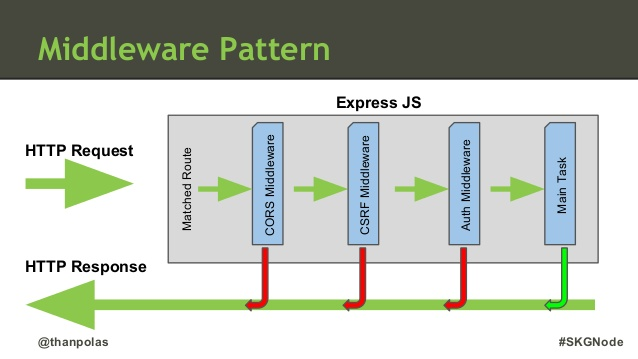
\includegraphics[width=15cm]{img/expressjsmiddleware.jpg}
  \captionof{figure}{Middleware trong ExpressJS}
\end{center}

Hình trên mô tả 3 middleware có trong ExpressJS. Một request khi gửi đến Express sẽ được xử lý qua 5 bước như sau :
\begin{itemize}
  \item Tìm Route tương ứng với request.
  \item Dùng CORS Middleware để kiểm tra cross-origin Resource sharing của request.
  \item Dùng CRSF Middleware để xác thực CSRF của request, chống fake request.
  \item Dùng Auth Middleware để xác thực request có được truy cập hay không.
  \item Xử lý công việc được yêu cầu bởi request (Main Task).
\end{itemize}

Bất kỳ bước nào trong các bước 2, 3, 4 nếu xảy ra lỗi sẽ trả về response thông báo cho người dùng, có thể là lỗi CORS, lỗi CSRF hay lỗi auth tùy thuộc vào request bị dừng ở bước nào.
\textbf{Middleware trong ExpressJS:} 

ExpressJS khi hoạt động, về cơ bản sẽ là một loạt các hàm Middleware được thực hiện liên tiếp nhau. Sau khi đã thiết lập, các request từ phía người dùng khi gửi lên ExpressJS sẽ thực hiện lần lượt qua các hàm Middleware cho đến khi trả về response cho người dùng. Các hàm này sẽ được quyền truy cập đến các đối tượng đại diện cho Request - req, Response - res, hàm Middleware tiếp theo - next, và đối tượng lỗi - err nếu cần thiết.

Một hàm Middleware sau khi hoạt động xong, nếu chưa phải là cuối cùng trong chuỗi các hàm cần thực hiện, sẽ cần gọi lệnh next() để chuyển sang hàm tiếp theo, bằng không xử lý sẽ bị treo tại hàm đó.

Các chức năng mà middleware có thể thực hiện trong ExpressJS sẽ bao gồm :
\begin{itemize}
  \item Thực hiện bất cứ đoạn code nào.
  \item Thay đổi các đối tượng request và response.
  \item Kết thúc một quá trình request-response.
  \item Gọi hàm middleware tiếp theo trong stack.
\end{itemize}

Trong Express, có 5 kiểu middleware có thể sử dụng :
\begin{itemize}
  \item Application-level middleware (middleware cấp ứng dụng).
  \item Router-level middleware (middlware cấp điều hướng - router).
  \item Error-handling middleware (middleware xử lý lỗi).
  \item Built-in middleware (middleware sẵn có).
  \item Third-party middleware (middleware của bên thứ ba).
\end{itemize}
\subsection{Sự lựa chọn}
Chúng ta có thể thấy Java là một ngôn ngữ mạnh, linh hoạt, bảo mật cao, viết một lần thực thi khắp nơi. Tuy nhiên vì Java chạy trên máy ảo Java Virtual machine, đây vừa là điểm mạnh khi Java có thể chỉ cần viết một lần thực thi khắp nơi, tuy nhiên nó cũng khiến Java chậm đi rất nhiều và tiêu thụ nhiều bộ nhớ, khiến cho ứng dụng ngày càng nặng nề khi xử lý nhiều kết nối.

Python là một ngôn ngữ rất dễ học, dễ sử dụng, có cú pháp đơn giản, cộng đồng hỗ trợ lớn, nhiều công cụ và công nghệ hỗ trợ. Đây cũng là ngôn ngữ mà được rất nhiều người yêu thích, tuy nhiên Python lại có những hạn chế như tốc độ khá chậm, chạy đơn luồng, vì vậy sẽ không thể đáp ứng được khi ứng dụng càng ngày càng có nhiều kết nối.

NodeJS có đặc điểm là tốc độ rất nhanh, xử lý nhiều kết nối tốt, dễ dàng mở rộng để phát triển, thích hợp. Đây là những đặc tính đặc biệt thích hợp cho hệ thống Tổ chức hành chính với những đặc thù công việc như hay thay đổi nghiệp vụ, xuất báo cáo định kỳ, theo yêu cầu, truy cập lượng lớn hồ sơ nhân viên. Vì vậy nhóm quyết định sử dụng NodeJS cùng với công nghệ ExpressJS cho phía server của hệ thống này.
\section{Cơ sở dữ liệu (Database)}
\textbf{Khái niệm:}

Cơ sở dữ liệu (Database) là một tập hợp các dữ liệu có tổ chức, thường được lưu trữ và truy cập điện tử từ hệ thống máy tính. Khi cơ sở dữ liệu phức tạp hơn, chúng thường được phát triển bằng cách sử dụng các kỹ thuật thiết kế và mô hình hóa chính thức.\\

\textbf{Phân loại:}
\begin{itemize}
    \item Cơ sở dữ liệu quan hệ (SQL)
    \item Cơ sở dữ liệu phi quan hệ (NoSQL)
\end{itemize}

\textbf{So sánh cơ sở dữ liệu quan hệ và phi quan hệ:}
\begin{table}[H]
	    \centering
	    \begin{tabular}{|p{3cm}|p{6cm}|p{6cm}|}
	    \hline
	    &Cơ sở dữ liệu quan hệ&Cơ sở dữ liệu phi quan hệ\\
	    \hline
	    Ngôn ngữ truy vấn&Ngữ truy vấn có cấu trúc&Sử dụng ngôn ngữ truy vấn không cấu trúc\\
	    \hline
	    Cấu trúc&Biểu thị dữ liệu dưới dạng bảng, hàng và cột&Biểu thị dữ liệu dưới dạng biểu đồ, các cặp khóa-giá trị và nhiều hơn thế.\\
	    \hline
	    Khả năng mở rộng&Mở rộng thêm chiều dọc&Mở rộng theo chiều ngang\\
	    \hline
	    Chi phí&Chi phí xây dựng và bảo trì cao&Khoảng 10\% so với cơ sở dữ liệu quan hệ\\
	    \hline
	    \end{tabular}
	    \caption{So sánh cơ sở dữ liệu quan hệ và phi quan hệ}
\end{table}
\subsection{Ngôn ngữ truy vấn có cấu trúc (SQL)}
\subsubsection{SQL là gì?}
SQL là loại ngôn ngữ máy tính, giúp cho thao tác lưu trữ và truy xuất dữ liệu được lưu trữ trong một cơ sở dữ liệu quan hệ. SQL là viết tắt của Structured Query Language là ngôn ngữ truy vấn có cấu trúc.

Tất cả RDBMS (hệ thống quản lý cơ sở dữ liệu quan hệ) như đều sử dụng SQL như là ngôn ngữ cơ sở dữ liệu chuẩn.

SQL là một ngôn ngữ được tiêu chuẩn hóa bởi ANSI (American National Standards Institute) – Viện tiêu chuẩn quốc gia Hoa Kỳ. Đây cũng đồng thời là ngôn ngữ được sử dụng phổ biến trong các hệ thống quản lý cơ sở dữ liệu quan hệ và hỗ trợ sử dụng trong các công ty lớn về công nghệ.
\subsubsection{Tại sao phải sử dụng SQL?}
SQL thường được các RDBMS sử dụng để tương tác với cơ sở dữ liệu thông qua các thao tác sau:
\begin{itemize}
    \item Tạo cơ sở dữ liệu, bảng và view mới.
    \item Để chèn các bản ghi vào trong một cơ sở dữ liệu.
    \item Để xóa các bản ghi từ một cơ sở dữ liệu.
    \item Để lấy dữ liệu từ một cơ sở dữ liệu.
\end{itemize}
\subsubsection{Chức năng}
Một trong những lý do khiến cho SQL được sử dụng phổ biến, chính là nó đã cho phép người dùng thực hiện đa dạng các chức năng sau:
\begin{itemize}
    \item Cho phép người dùng truy cập dữ liệu trong các hệ thống quản lý cơ sở dữ liệu quan hệ.
    \item Cho phép người dùng mô tả dữ liệu.
    \item Cho phép người dùng xác định dữ liệu trong cơ sở dữ liệu và thao tác dữ liệu đó.
    \item Cho phép nhúng trong các ngôn ngữ khác sử dụng mô-đun SQL, thư viện và trình biên dịch trước.
    \item Cho phép người dùng tạo và thả các cơ sở dữ liệu và bảng.
    \item Cho phép người dùng tạo chế độ view, thủ tục lưu trữ, chức năng trong cơ sở dữ liệu.
    \item Cho phép người dùng thiết lập quyền trên các bảng, thủ tục và view.
\end{itemize}
\subsubsection{Ưu điểm}
\begin{itemize}
    \item Dữ liệu có ở mọi nơi: Dữ liệu xuất hiện ở mọi nơi trên màn hình từ laptop đến điện thoại của bạn. Việc học tập và tìm hiểu SQL sẽ giúp bạn biết được cách thức hoạt động của những dữ liệu này.
    \item Thêm, sửa, đọc và xóa dữ liệu dễ dàng: với SQL, các thao tác xử lý dữ liệu trở nên dễ dàng hơn bao giờ hết. Bạn chỉ cần thực hiện một số thao tác với dữ liệu đơn giản trên SQL thay vì phải dùng nhiều câu lệnh phức tạp trên các loại ngôn ngữ khác.
    \item SQL giúp công việc lập trình dễ dàng hơn: bạn có thể lưu nhiều dữ liệu cho nhiều ứng dụng khác nhau trên cũng một cơ sở dữ liệu và việc truy cập các cơ sở dữ liệu này trở lên đơn giản hơn nhờ một cách thức giống nhau.
    \item Được sử dụng và hỗ trợ bởi nhiều công ty lớn: tất cả các công ty lớn về công nghệ trên thế giới hiện nay như Microsoft, IBM, Oracle… đều hỗ trợ việc phát triển ngôn ngữ SQL.
    \item Lịch sử hơn 40 năm: với lịch sử phát triển hơn 40 năm từ 1970, SQL vẫn tồn tại và trụ vững đến ngày nay. Điều này cho thấy vị trí của SQL hiện tại rất khó bị thay thế bởi bất kỳ một ngôn ngữ máy tính nào khác.
\end{itemize}
\subsection{Hệ cơ sở dữ liệu quan hệ (RDBMS)}
\textbf{Khái niệm:}

RDBMS - Relational Database Management System - là hệ cơ sở dữ liệu quan hệ. Tất cả các hệ thống quản trị cơ sở dữ liệu hiện đại như SQL, MySQL, MS SQL Server, Oracle, ... đều dựa trên RDBMS.

Hệ thống quản lý cơ sở dữ liệu quan hệ (RDBMS) là một hệ thống quản lý cơ sở dữ liệu (DBMS) dựa trên mô hình quan hệ được giới thiệu bởi EF Codd.\\

\textbf{Bảng (Table):}

RDBMS sử dụng các bảng để lưu trữ dữ liệu. Mỗi bảng là một tập hợp các dữ liệu có liên quan đến nhau và có nhiều hàng và cột để lưu dữ liệu. Bảng là hình thức lưu trữ phổ biến và đơn giản nhất trong môt cơ sở dữ liệu quan hệ. Ví dụ về bảng một nhóm môn học trong bảng MONHOC sau đây:\\
\begin{table}[H]
    \centering
    \begin{tabular}{|l|l|l|}
    \hline
         \textbf{ID}&\textbf{TEN\_MON\_HOC}&\textbf{SO\_TIN\_CHI}\\
         \hline
         1&Giải tích 1&4\\
		\hline
		2&Vật lý&3\\
		\hline			
		3&Kỹ thuật lập trình&4\\
		\hline
    \end{tabular}
    \caption{Ví dụ về bảng dữ liệu}
\end{table}

\textbf{Trường (Field):}
	
	Mỗi bảng được chia thành các thực thể nhỏ gọi là các trường, chứa các thông tin cụ thể về mỗi bản ghi trong bảng. Các trường trong bảng MONHOC bao gồm: ID, TEN\_MON\_HOC, SO\_TIN\_CHI.\\
	\begin{table}[H]
	    \centering
	    \begin{tabular}{|l|}
	        \hline
	        \textbf{TEN\_MON\_HOC}\\
	        \hline
	        Giải tích 1\\
	        \hline
	        Vật lý\\
	        \hline
	        Kỹ thuật lập trình\\
	        \hline
	    \end{tabular}
	    \caption{Ví dụ một trường trong bảng dữ liệu}
	\end{table}
	
\textbf{Hàng hoặc bản ghi (Record):}
	
Một hàng của bảng được gọi là bản ghi , nó chứa thông tin của một đối tượng trong bảng. Ví dụ ở bảng MONHOC có 3 bản ghi. Sau đây là một bản ghi trong bảng:\\
\begin{table}[H]
    \centering
    \begin{tabular}{|r|r|r|}
        \hline
		1&Giải tích 1&4\\
		\hline
    \end{tabular}
    \caption{Ví dụ về một bản ghi}
\end{table}

\textbf{Ràng buộc (Constraint):}

Ràng buộc là các quy tắc cho các cột dữ liệu trong bảng. Chúng được sử dụng để giới hạn loại dữ liệu có thể insert vào một bảng. Điều này đảm bảo tính chính xác và độ tin cậy của dữ liệu trong cơ sở dữ liệu.\\
Constraint có thể là cấp độ cột hoặc cấp độ bảng. Các ràng buộc cấp độ cột chỉ được áp dụng cho một
cột trong khi các ràng buộc mức bảng được áp dụng cho toàn bộ bảng.\\
Sau đây là một số ràng buộc phổ biến nhất được sử dụng trong SQL :\\
\begin{table}[H]
    \centering
    \begin{tabular}{|l|l|}
        \hline
         NOT NULL&Đảm bảo rằng một field không có giá trị NULL  \\
         \hline
         DEFAULT&Cung cấp giá trị mặc định của một field khi không được xác định\\
         \hline
         UNIQUE&Đảm bảo giá trị trong một field là khác nhau\\
         \hline
         PRIMARY Key&Mỗi record là duy nhất trong một bảng cơ sở dữ liệu\\
         \hline
         FOREIGN Key&Mỗi record là duy nhất trong trong bất kỳ bảng cơ sở dữ liệu khác\\
         \hline
         CHECK&Đảm bảo rằng tất cả các giá trị trong một cột thỏa mãm một số điều kiện\\
         \hline
         INDEX&Dùng để tạo và lấy dữ liệu một cách nhanh chóng\\
         \hline
    \end{tabular}
    \caption{Một số ràng buộc phổ biến trong SQL}
\end{table}
\subsection{Hệ quản trị cơ sở dữ liệu}

Hệ quản trị cơ sở dữ liệu (Database Management System - DBMS) là hệ thống kiểm soát việc lưu trữ, tổ chức và truy xuất dữ liệu.

Mỗi DBMS đều có thành phần gọi là Query Language (Ngôn ngữ truy vấn), các ứng dụng muốn truy cập dữ liệu đều phải nhờ vào thành phần này.

Các hệ quản trị cơ sở dữ liệu quan hệ phổ biến nhất hiện nay:
\subsubsection{Oracle Database}
\begin{center}
  \captionsetup{type=figure}
  
\includegraphics[scale=0.4]{img/oracle.jpg}
  \captionof{figure}{Oracle Database}
\end{center}


\textbf{Oracle là gì?}


Oracle Database hay còn gọi là Oracle RDBMS hoặc đơn giản là Oracle là 1 hệ quản trị cơ sở dữ liệu quan hệ, được phát triển và phân phối bởi tập đoàn Oracle

Cơ sở dữ liệu Oracle là cơ sở dữ liệu đầu tiên được thiết kế cho điện toán lưới doanh nghiệp, cách linh hoạt và tiết kiệm chi phí nhất để quản lý thông tin và ứng dụng. Điện toán lưới doanh nghiệp tạo ra các nhóm lớn máy chủ và lưu trữ mô-đun theo tiêu chuẩn công nghiệp. Với kiến trúc này, mỗi hệ thống mới có thể được cung cấp nhanh chóng từ nhóm các thành phần. Không cần khối lượng công việc cao nhất, bởi vì công suất có thể dễ dàng được thêm hoặc phân bổ lại từ các nguồn tài nguyên khi cần thiết.\\

\textbf{Đặc điểm của Oracle}
\begin{itemize}
    \item Quản lý được hệ thống dữ liệu lớn
    \item Hỗ trợ nhiều công cụ để quản trị cũng như nhập, xuất dữ liệu dễ dàng
    \item Có thể hoạt động trên nhiều hệ điều hành khác nhau như Windows, Linux, Mac OS, Unix,...
    \item Truy cập đồng thời
    \item Hỗ trợ cơ chế khóa
    \item Thực thi song song
    \item Tính khả chuyển
\end{itemize}

\textbf{Thế mạnh của Oracle:}
\begin{itemize}
    \item \textit{Hệ thống quản lý và kiểm soát tập trung:} Điều này cho phép dữ liệu được kiểm soát hoàn toàn từ một trao đổi dạng bảng vì nó chịu trách nhiệm gán, thêm, xóa các bản ghi và sửa đổi chúng.
    \item \textit{Tiêu chuẩn hóa:} Cho phép tiêu chuẩn hóa giữa các triển khai SQL khác nhau.
    \item \textit{Nhóm các giao dịch:} Nó cho phép nhóm một số giao dịch và chia từng hoạt động thành các phân khúc và do đó đạt được hiệu suất tốt hơn trong thời gian ngắn hơn có thể.
    \item \textit{Phương thức hiệu suất:} Áp dụng các phương pháp để cải thiện cơ sở dữ liệu thông qua ứng dụng Cluster.
\end{itemize}
\subsubsection{MySQL}
\begin{center}
  \captionsetup{type=figure}
    
\includegraphics[scale=0.5]{img/mysql.jpg}
  \captionof{figure}{MySQL}
\end{center}

MySQL là một hệ quản trị cơ sở dữ liệu quan hệ mã nguồn mở, được phát triển, phân phối và hỗ trợ bởi tập đoàn Oracle.\\

\textbf{MySQL hoạt động như thế nào?}

MySQL hoạt động dưới hình thức client-server:
\begin{itemize}
    \item MySQL tạo một cơ sở dữ liệu để lưu trữ và thao tác dữ liệu, xác định mối quan hệ của từng bảng.
    \item Khách hàng có thể thực hiện các yêu cầu bằng cách nhập các câu lệnh SQL cụ thể trên MySQL.
    \item Ứng dụng máy chủ sẽ phản hồi với thông tin được yêu cầu và nó sẽ xuất hiện ở phía máy khách.
\end{itemize}


\textbf{Đặc điểm và thế mạnh:}
\begin{itemize}
    \item \textit{Tính nội bộ và linh động:}
    \begin{itemize}
    \item Viết bằng C và C++
    \item Đã thử nghiệm với một loạt các trình biên dịch khác nhau
    \item Hoạt động trên nhiều nền tảng khác nhau
    \item Sử dụng thiết kế máy chủ nhiều lớp với các mo-đun độc lập
    \item Được thiết kế để đa luồng hoàn toàn bằng cách sử dụng các luồng nhân, để dễ dàng sử dụng nhiều CPU nếu chúng có sẵn
    \item Triển khai các bảng băm trong bộ nhớ, được sử dụng làm bảng tạm thời.
    \item Triển khai các hàm SQL bằng cách sử dụng thư viện lớp được tối ưu hóa cao nhất phải nhanh nhất có thể
    \end{itemize}
    \item \textit{Bảo mật}
    \begin{itemize}
        \item Một hệ thống đặc quyền và mật khẩu rất linh hoạt và an toàn, và cho phép xác minh dựa trên máy chủ
        \item Bảo mật mật khẩu bằng cách mã hóa tất cả lưu lượng mật khẩu khi bạn kết nối với máy chủ.
    \end{itemize}
    \item \textit{Khả năng mở rộng và giới hạn:}
    \begin{itemize}
        \item Hỗ trợ cơ sở dữ liệu lớn
        \item Hỗ trợ lên đến 64 chỉ mục cho mỗi bảng
    \end{itemize}
    \item \textit{Ổn định, có tốc độ cao và dễ sử dụng}
    \item \textit{Đa tính năng:} Hỗ trợ rất nhiều chức năng SQL
\end{itemize}
\subsubsection{SQL Server}
\begin{center}
  \captionsetup{type=figure}
    
\includegraphics[scale=0.3]{img/sql-server.png}
  \captionof{figure}{SQL Server}
\end{center}
\textbf{SQL Server là gì?}

SQL Server là một RDBMS được phát triển bởi tập đoàn Microsoft. Tương tự như phần mềm RDBMS khác, SQL Server được xây dựng dựa trên SQL, một ngôn ngữ lập trình tiêu chuẩn để tương tác với các cơ sở dữ liệu quan hệ. Máy chủ SQL được liên kết với Transact-SQL hoặc T-SQL, triển khai SQL Microsoft Microsoft bổ sung một tập hợp các cấu trúc lập trình độc quyền. SQL Server hoạt động độc quyền trên môi trường Windows trong hơn 20 năm. Năm 2016, Microsoft đã cung cấp nó trên Linux. SQL Server 2017 thường có sẵn vào tháng 10 năm 2016 chạy trên cả Windows và Linux.\\
\newline
\textbf{SQL Server hoạt động như thế nào?}
\begin{itemize}
    \item Giống như các công nghệ RDBMS khác, SQL Server chủ yếu được xây dựng xung quanh cấu trúc bảng dựa trên hàng để kết nối các thành phần dữ liệu liên quan trong các bảng khác nhau với nhau, tránh việc lưu trữ dữ liệu ở nhiều nơi trong cơ sở dữ liệu. Mô hình quan hệ cũng cung cấp tính toàn vẹn tham chiếu và các ràng buộc toàn vẹn khác để duy trì độ chính xác của dữ liệu. Các kiểm tra này là một phần của việc tuân thủ rộng hơn các nguyên tắc về tính nguyên tử, tính nhất quán, độ cô lập và độ bền, được gọi chung là các thuộc tính ACID và được thiết kế để đảm bảo rằng các giao dịch cơ sở dữ liệu được xử lý một cách đáng tin cậy.
    \item Thành phần cốt lõi của SQL Server là SQL Server Database Engine, điều khiển lưu trữ, xử lý và bảo mật dữ liệu. Nó bao gồm một công cụ quan hệ xử lý các lệnh và truy vấn và một công cụ lưu trữ quản lý các tệp cơ sở dữ liệu, bảng, trang, chỉ mục, bộ đệm dữ liệu và giao dịch. Các thủ tục lưu trữ, kích hoạt, khung nhìn và các đối tượng cơ sở dữ liệu khác cũng được tạo bởi Cơ sở dữ liệu.
    \item Bên dưới cơ sở dữ liệu là Hệ điều hành Máy chủ SQL hoặc SQLOS. SQLOS xử lý các chức năng cấp thấp hơn, chẳng hạn như quản lý bộ nhớ và I/O, lập lịch công việc và khóa dữ liệu để tránh các cập nhật xung đột. Một lớp giao diện mạng nằm phía trên Cơ sở dữ liệu và sử dụng giao thức Luồng dữ liệu dạng bảng của Microsoft để tạo điều kiện cho các tương tác yêu cầu và phản hồi với các máy chủ cơ sở dữ liệu. Và ở cấp độ người dùng, các DBA và nhà phát triển SQL Server viết các câu lệnh T-SQL để xây dựng và sửa đổi cấu trúc cơ sở dữ liệu, thao tác dữ liệu, thực hiện bảo vệ an ninh và sao lưu cơ sở dữ liệu, trong số các tác vụ khác
\end{itemize}
\textbf{Thế mạnh:}
\begin{itemize}
    \item Cho phép nhiều người dùng chung một cơ sở dữ liệu
    \item Duy trì lưu trữ bền vững
    \item Khả năng mở rộng
    \item Tính bảo mật cao
    \item Độ tin cậy, bảo vệ dữ liệu
    \item Hỗ trợ phân tích dữ liệu
    \item Kết hợp tốt với các sản phẩm của Microsoft
    \item Có thể sao lưu, khôi phục dữ liệu một cách dễ dàng
\end{itemize}

\subsubsection{PostgreSQL}
\begin{center}
  \captionsetup{type=figure}
    
\includegraphics[scale=0.5]{img/postgre-sql.jpg}
  \captionof{figure}{PostgreSQL}
\end{center}

PostgreSQL là một RDBMS mở nguồn mở được xây dựng trên mã nguồn ban đầu của đại học Berkeley.

\textit{Đặc điểm và thế mạnh:}
\begin{itemize}
    \item Truy xuất dữ liệu tốc độ nhanh
    \item Sử dụng câu truy vấn phức tạp
    \item Sử dụng khóa ngoại
    \item Có thủ tục
    \item Đảm bảo tính toàn vẹn của các giao tác
\end{itemize}

\subsection{Hệ cơ sở dữ liệu phi quan hệ (Non-RDBMS)}
Hệ cơ sở dữ liệu phi quan hệ là cơ sở dữ liệu không sử dụng mô hình bảng gồm các cột và hàng như nhiều hệ cơ sở dữ liệu truyền thống. Thay vào đó, Non-RDBMS sử dụng mô hình lưu trữ được tối ưu hóa cho các yêu cầu cụ thể của loại dữ liệu được lưu trữ. Cơ sở dữ liệu phi quan hệ (Non-relational database) phổ biến nhất được gọi là NoSQL.\\
Các Non-RDBMS phổ biến:
\subsubsection{MongoDB}
\begin{center}
  \captionsetup{type=figure}
    
\includegraphics[width=10cm]{img/mongo.png}
  \captionof{figure}{MongoDB}
\end{center}

MongoDB là một hệ quản trị cơ sở dữ liệu mã nguồn mở và là cơ sở dữ liệu NoSQL hàng đầu, được nhiều người sử dụng.

Các thuật ngữ thường sử dụng trong MongoDB:
\begin{itemize}
    \item \textbf{\_id:} Là trường bắt buộc có trong mỗi document. Trường \_id đại diện cho một giá trị duy nhất trong document MongoDB. Trường \_id cũng có thể được hiểu là khóa chính trong document. Nếu bạn thêm mới một document thì MongoDB sẽ tự động sinh ra một \_id.
    \item \textbf{Collection:} Là nhóm của nhiều document trong MongoDB, tương ứng với một bảng trong RDBMS
    \item \textbf{Cursor:} Đây là một con trỏ đến tập kết quả của một truy vấn. Máy khách có thể lặp qua một con trỏ để lấy kết quả.
    \item \textbf{Database:} Nơi chứa các Collection.
    \item \textbf{Document:} Là một bản ghi thuộc một Collection.
    \item \textbf{Field:} Là một cặp name-value trong một document.
\end{itemize}

\textit{Thế mạnh:}
\begin{itemize}
    \item Ít schema hơn
    \item Cấu trúc của một đối tượng rõ ràng
    \item Không có các phép join phức tạp
    \item Khả năng mở rộng cực lớn: Việc mở rộng dữ liệu mà không cần phải quan tâm đến các vấn đề như khóa ngoại, khóa chính, kiểm tra ràng buộc,...
    \item Sử dụng bộ nhớ trong để lưu giữ cửa sổ làm việc cho phép truy cập dữ liệu nhanh hơn. Việc cập nhật được thực hiện nhanh gọn nhờ update tại chỗ (in-place).
    \item Hỗ trợ nhiều công cụ lưu trữ
\end{itemize}

\textit{Các thao tác cơ bản trong MongoDB}
\begin{description}
\item 1.Create:\\
Tạo hoặc thêm một document mới vào collection, nếu collection đó chưa tồn tại thì sẽ tạo mới collection

MongoDB cung cấp hai phương thức để chèn thêm một document:
\begin{itemize}
    \item db.collection.insertOne(): chèn một tài liệu mới vào một collection. Nếu document không có trường \_id , MongoDB sẽ tự động thêm trường \_id với value kiểu ObjectId.
\begin{verbatim}
db.inventory.insertOne(
    { item: "canvas", qty: 100, tags: ["cotton"], size:{ h: 28, w: 35.5}}
)
\end{verbatim}
    \item db.collection.insertMany(): chèn nhiều document vào một collection, truyền vào phương thức là mảng các document
\begin{verbatim}
db.inventory.insertMany([
    {item: "journal", qty: 25, tags: ["blank", "red"], size:{h: 14, w: 21}},
    {item: "mat", qty: 85, tags: ["gray"], size:{h: 27.9, w: 35.5}},
    {item: "mouse", qty: 25, tags: ["gel", "blue"], size:{h: 19, w: 22.85}}
])
\end{verbatim}
\end{itemize}
\item 2.Read\\
Truy xuất document từ một collection. Để lấy ra toàn bộ document của ta sử dụng phương thức find
\begin{verbatim}
        db.inventory.find()
\end{verbatim}
\item 3. Update\\
Thao tác update cho phép chình sửa document trong collection
\begin{itemize}
    \item Cập nhật một document với db.collection.updateOne():
    \begin{verbatim}
        db.inventory.updateOne(
           { item: "paper" },
           {
             $set: { "size.uom": "cm", status: "P" }
           }
        )
    \end{verbatim}
    \item Cập nhật nhiều Document với db.collection.updateMany():
    \begin{verbatim}
        db.inventory.updateMany(
           { "qty": { $lt: 50 } },
           {
             $set: { "size.uom": "in", status: "P" },
             $currentDate: { lastModified: true }
           }
        )
    \end{verbatim}
    \item Thay thế một document: Để thay thế toàn bộ nội dung của một document (ngoại trừ trường \_id), truyền vào toàn bộ document mới là một tham số thứ hai của hàm. Ví dụ dưới đây thay thế document đầu tiên từ collection inventory mà có item bằng "paper"
\begin{verbatim}
db.inventory.replaceOne(
    {item:"paper"},
    {item: "paper",instock:[{warehouse:"A",qty:60},{warehouse:"B",qty:40}]}
)
\end{verbatim}
\end{itemize}
\item 4. Delete\\
\begin{itemize}
    \item Xóa một document thỏa mãn điều kiện: Để xóa chỉ một document phù hợp với điều kiện (trường hợp có nhiều document thỏa mãn thì sẽ xóa document đầu tiên), sử dụng db.collection.deleteOne(filter)
    \item Xóa tất cả document thỏa mãn điều kiện: sử dụng db.collection.deleteMany(filter)

\end{itemize}
\end{description}

\subsubsection{Neo4j}
\begin{center}
  \captionsetup{type=figure}
  
\includegraphics[width=10cm]{img/neo4j.png}
  \captionof{figure}{Neo4j}
\end{center}

Neo4j là hệ quản trị cơ sở dữ liệu đồ thị đầu tiên được giới thiệu vào năm 2007 và công bố phiên bản 1.0 vào năm 2010. Hiện nay Neo4j là một trong những hệ quản trị cơ sở dữ liệu đồ thị được sử dụng nhiều nhất.

\textit{Đặc điểm:} Các đối tượng được miêu tả dưới dạng các đỉnh của đồ thị, các thuộc tính của đối tượng được miêu tả bằng liên kết có hướng đến một đối tượng khác.

\textit{Thế mạnh:}
\begin{itemize}
    \item Khả năng mở rộng cao
    \item Phân tích dữ liệu theo thời gian thực
    \item Thời gian thực thi nhanh
\end{itemize}
\subsubsection{Cassandra}
\begin{center}
  \captionsetup{type=figure}
  
\includegraphics[width=10cm]{img/cassandra.png}
  \captionof{figure}{Cassandra}
\end{center}

Cassandra ban đầu được tạo ra bởi Facebook. Sau đó nó đã được tặng cho Quỹ Apache và tháng 2 năm 2010 và được nâng cấp lên thành dự án hàng đầu của Apache. Cassandra là một cơ sở dữ liệu phân tán kết hợp mô hình dữ liệu của Google Bigtable với thiết kế hệ thống phân tán như bản sao của Amazon Dynamo.\\

\textit{Đặc điểm và thế mạnh:}
\begin{itemize}
    \item Tính phân tán và không tập trung (distributed and decentralized): Khả năng phân chia dữ liệu thành nhiều phần, đặt trên nhiều node khác nhau trong khi người dùng vẫn nhận thấy dữ liệu này là một khối thống nhất.
    \item Tính mềm dẻo (elastic scalability): Hệ thống có thể dễ dàng mở rộng số node trong cluster để có thể phục vụ số lượng request lớn và rút bớt số node khi số lượng request giảm.
    \item Tính sẵn sàng cao (high availability): Dữ liệu được sao lưu thành nhiều bản và được chia thành nhiều node. Điều này mang lại khả năng đáp ứng ngay lập tức cho Cassandra khi Client thực hiện tác vụ đọc hay ghi bằng cách thực hiện trên bản sao gần nhất hoặc trên tất cả các bản sao.
    \item Tính nhất quán (consistance): trong Cassandra, dữ liệu sẽ nhất quán sau một khoảng thời gian nào đó chứ không phải được nhất quán ngay sau khi người dùng ghi dữ liệu
    \item Tính chấp nhận lỗi (fault tolerance): Do dữ liệu được sao chép thành nhiều bản trên các node của cluster nên kể cả khi dữ liệu ở một node nào đó bị lỗi, ta vẫn có thể truy xuất dữ liệu của mình trên một node khác.
    \item Tính hướng cột (column oriented key-value store): Các RDBMS hướng dòng (row-oriented) phải định nghĩa trước các cột (column) trong các bảng (table). Đối với Cassandra ta không phải làm điều đó, đơn giản là thêm vào bao nhiêu cột cũng được tùy theo nhu cầu của ta.
    \item Hiêụ năng cao (high performance): Cassandra được thiết kế riêng biệt từ sơ khai cho đến khi đầy đủ lợi ích cho máy đa luồng/đa lõi và được chạy trên hàng chục những máy được đặt trong các trung tâm dữ liệu với quy mô nhất quán và liên tục với hàng trăm terabyte dữ liệu.
\end{itemize}
\subsubsection{Redis}
\begin{center}
  \captionsetup{type=figure}
  
\includegraphics[width=10cm]{img/redis.png}
  \captionof{figure}{Redis}
\end{center}


\textbf{Redis là gì?}\\

Redis (REmote DIctionary Server) là một mã nguồn mở được dùng để lưu trữ dữ liệu có cấu trúc, có thể sử dụng như một cơ sở dữ liệu, bộ nhớ cache hay một message broker. Nó là hệ thống lưu trữ dữ liệu với dạng KEY-VALUE rất mạnh mẽ và phổ biến hiện nay.
Bên cạnh lưu trữ key-value trên RAM giúp tối ưu hiệu năng, Redis còn có cơ chế sao lưu dữ liệu trên đĩa cứng cho phép phục hồi dữ liệu khi gặp sự cố.
Redis cung cấp thời gian phản hồi ở tốc độ chưa đến một mili giây, giúp thực hiện hàng triệu yêu cầu mỗi giây cho các ứng dụng thời gian thực.
Redis thường được chọn sử dụng cho hoạt động lưu trữ bộ nhớ đệm, quản lý phiên, trò chơi, bảng xếp hạng, phân tích theo thời gian thực.\\

\textbf{Redis hoạt động như thế nào?}\\

Toàn bộ dữ liệu Redis nằm trong bộ nhớ, trái với cơ sở dữ liệu thông thường lưu dữ liệu trên ổ đĩa. Bằng cách loại bỏ sự cần thiết phải truy cập ổ đĩa, kho dữ liệu bộ nhớ như Redis tránh được sự chậm trễ do thời gian tìm kiếm và có thể truy cập dữ liệu trong vài micro giây. Redis có cấu trúc dữ liệu linh hoạt, độ khả dụng cao, dữ liệu trên Ram, hộ trợ lưu trữ trên ổ đĩa, cluster giúp xây dựng các ứng dụng quy mô lớn theo thời gian thực.\\

\textbf{Đặc điểm của Redis}\\
\begin{itemize}
    \item Kho dữ liệu trong bộ nhớ: Toàn bộ dữ liệu Redis nằm trong bộ nhớ chính của máy chủ, trái với cơ sở dữ liệu thông thường phần lớn các tác vụ đều yêu cầu truy cập qua lại tới ổ đĩa, kho dữ liệu trong bộ nhớ như Redis không phải mất thời gian cho truy cập ỗ đĩa, do đó kho dữ liệu này có thể hộ trợ thêm khá nhiều tác vụ và có thời gian phản hổi nhanh hơn. Kết quả là hiệu suất nhanh thấy rõ với các tác vụ đọc hoặc ghi thông thường, hộ trợ hàng triệu tác vụ mỗi giây.
    \item Cấu trúc dữ liệu linh hoạt
    \item Đơn giản và dễ sử dụng: Redis đơn giản hóa bằng cách cho phép bạn viết ít dòng lệnh hơn để lưu trữ, truy cập và sử dụng dữ liệu trên ứng dụng. Ví dụ nếu ứng dụng của bạn có dữ liệu được lưu trên một mảng băm và bạn muốn lưu dữ liệu đó trên kho dữ liệu, bạn chỉ cần sử dụng cấu trúc dữ liệu mã hash của Redis. Tác vụ tương tự trên kho dữ liệu không có cấu trúc dữ liệu hash sẽ cần nhiều dòng mã để chuyển đổi từ định dạng này sang định dạng khác. Redis được trang bị cấu trúc dữ liệu riêng và nhiều tùy chọn để điều khiển và tương tác với dữ liệu của bạn. Có nhiều ngôn ngữ hộ trỡ Redis như Java, Python, PHP, JavaScript, Nodejs...
    \item Sao chép và độ bền: Redis sử dụng kiến trúc bản Master-Slave và hộ trỡ sao chép không đồng bộ trong đó có thể sao chép dữ liệu sang nhiều máy chủ bản sao. Việc này mang lại hiệu suất đọc cao hơn vì có thể chia tách các yêu cầu giữa các máy chủ và tốc độ khôi phục nhanh hơn khi máy chủ gặp sự cố. Về độ bền Redis hộ trợ sao lưu sang ổ đĩa tại một thời điểm nào đó.
    \item Khả năng mở rộng: Redis là dự án mã nguồn mở được một cộng đồng đông đảo ủng hộ. Không có giới hạn về nhà cung cấp hoặc công nghệ vì Redis có tính tiêu chuẩn mở, hộ trợ định dạng dữ liệu mở và tập hợp các máy chủ.
\end{itemize}

\textbf{Redis được sử dụng ở đâu?}
\begin{itemize}
    \item Lưu trữ bộ nhớ đệm: Redis có thể phục vụ những mục dữ liệu thường xuyên được yêu cầu với thời gian phản hồi chưa đến một mili giây và cho phép bạn dễ dàng thay đổi quy mô nhằm đáp ứng mức tải cao hơn mà không cần gia tăng phần backend có chi phí tốn kém hơn. Một số ví dụ phổ biến về nhớ đệm khi sử dụng Redis bao gồm nhớ đệm kết quả truy vấn cơ sở dữ liệu, nhớ đệm phiên lâu bền, nhớ đệm trang web và nhớ đệm các đối tượng thường xuyên được sử dụng như ảnh, tập tin và siêu dữ liệu.
    \item Trò chuyện, nhắn tin và danh sách xử lý tác vụ: Redis với cơ chế Pub/Sub là cấu trúc gửi nhận tin nhắn trong Redis cho phép Redis hộ trợ các room chat hiệu suất cao theo thời gian thực. Cấu trúc dữ liệu dạnh list giúp dễ dàng triển khai một danh sách các tác vụ cần xử lý có tải trọng nhẹ.
    \item Lưu trữ session: Redis là kho dữ liệu trong bộ nhớ có độ khả dụng và độ bền cao, được dùng để lưu trữ và quản lý session cho các ứng dụng internet. Redis có độ trễ thấp, quy mô, độ đàn hồi cần thiết để quản lý dữ liệu session như thông tin đăng nhập, trạng thái session.
\end{itemize}
\subsection{So sánh Relational Database và Non-Relational Database}
\begin{table}[H]
	    \centering
	    \begin{tabular}{|p{3cm}|p{6cm}|p{6cm}|}
	        \hline
	        &\textbf{Relational}&\textbf{Non-Relational}\\
	        \hline
	        Ngôn ngữ truy vấn&Ngôn ngữ truy vấn có cấu trúc &Truy vấn đối tượng: trực quan, chuyển một tài liệu để giải thích những gì bạn đang truy vấn\\
	        \hline
	        Kiểu dữ liệu&Lưu các kiểu dữ liệu được quy định&Có thể lưu bất kỳ loại dữ liệu nào\\
	        \hline
	        Khả năng mở rộng&Mở rộng thêm chiều dọc&Mở rộng theo chiều ngang\\
	        \hline
	        Hiển thị dữ liệu&Dưới dạng bảng và hàng&Dưới dạng JSON\\
	        \hline
	        Chi phí&Chi phí xây dựng và bảo trì cao&Khoảng 10\% so với Relational\\
	        \hline
	    \end{tabular}
	    \caption{So sánh cơ sở dữ liệu quan hệ và cơ sở dữ liệu phi quan hệ}
	\end{table}
\subsection{Kết luận và lựa chọn}
Dựa vào các đối tượng mà hệ thống hướng tới, hệ thống cần lưu trữ lượng dữ liệu lớn, bao gồm các dữ liệu có thuộc tính cố định lẫn các tập dữ liệu có thuộc tính thay đổi theo thời gian. Vì vậy, sử dụng kết hợp giữa hệ cơ sở dữ liệu quan hệ và hệ cơ sở dữ liệu phi quan hệ là hợp lý. Với những phân tích đánh giá như trên, nhóm quyết định lựa chọn sửa dụng đồng thời \textbf{MongoDB} và \textbf{Oracle}. Bên cạnh đó, hệ thống cần một bộ lưu trữ cache với tốc độ  cao, vì thế nhóm lựa chọn \textbf{Redis} để thực hiện lưu trữ cache cho hệ thống
\newpage
\chapter{\textbf{PHÂN TÍCH YÊU CẦU ĐỀ TÀI}}
\newpage
\section{Phân quyền người dùng trong hệ thống}
Dựa vào những yêu cầu thực tế của hệ thống và những khảo sát thực tế đối với các cá nhân có nhu cầu sử dụng, xây dựng hệ thống Tổ chức - Hành chính. Nhóm đưa ra các vai trò, người dùng chính trong hệ thống như sau:
\begin{itemize}
    \item Quản trị hệ thống
    \item Cán bộ quản lý phòng Tổ chức - Hành chính
    \item Cán bộ phòng Tổ chức - Hành chính
    \item Cán bộ, nhân viên, giáo viên của trường
\end{itemize}
\section{Những chức năng mà hệ thống đảm nhiệm}
\begin{itemize}
    \item Quản lý thông tin cán bộ công nhân viên nhà trường
    \begin{itemize}
        \item Tính năng tìm kiếm, thêm, xoá, sửa, lưu thông tin.
        \item Tính năng nhập dữ liệu từ file Excel.
        \item Quản lý lý lịch, thời gian công tác, ngày nghỉ, trình độ.
        \item Tính năng truy vấn dữ liệu, xuất dữ liệu theo yêu cầu. 
    \end{itemize}
    \item Website truyền thông với các tin tức mới nhất, giao diện đẹp, dễ sử dụng.
    \begin{itemize}
        \item Thực hiện thiết kế UI, UX hợp lý.
        \item Có công cụ để viết bài, tin tức mới. Công cụ này phải thân thiện, dễ sử dụng.
        \item Có công cụ liên kết với các phòng ban khác, nhận dữ liệu tin tức từ các trang phòng ban khác của trường.
    \end{itemize}
    \item Các tính năng thống kê như tính điểm thi đua, điểm thưởng,...
    \begin{itemize}
        \item Hiện thực các công cụ thống kê.
        \item Hỗ trợ tính các tính năng chuyên môn như tính điểm thi đua, tính điểm thưởng.
    \end{itemize}
    \item Quản lý bảo hiểm cho cán bộ.
    \begin{itemize}
        \item Thực hiện lưu trữ, cập nhật dữ liệu bảo hiểm cho cán bộ.
        \item Có công cụ nhắc nhở những cán bộ sắp hết hạn bảo hiểm.
        \item Có công cụ để truy xuất lịch sử mua bảo hiểm của cán bộ.
    \end{itemize}
    \item Quản lý các cấp, đơn vị hành chính của nhà trường.
    \begin{itemize}
        \item Thực hiện lưu trữ các cấp, đơn vị hành chính hiện tại của nhà trường.
        \item Có công cụ để thực hiện cập nhật, thêm mới, xoá các đơn vị.
        \item Có công cụ để truy xuất các đơn vị hiện tại của nhà trường.
    \end{itemize}
    \item Quản lý quy trình khen thưởng.
    \begin{itemize}
        \item Quản lý các huân chương, bằng khen của cán bộ nhân viên.
        \item Quản lý các cấp khen thưởng như cấp trường, Thành phố, cấp Bộ \& nhà nước,...
        \item Quản lý thời gian khen thưởng.
    \end{itemize}
    \item Quản lý quy trình kỷ luật.
    \begin{itemize}
        \item Quản lý các hình thức kỷ luật, lý do kỷ luật của cán bộ nhân viên.
        \item Quản lý các cấp kỷ luật như cấp trường, Đảng,...
        \item Quản lý ghi chú khiếu nại về kỷ luật.
    \end{itemize}
    \item Quản lý lương cán bộ.
    \begin{itemize}
        \item Quản lý thông tin lương của các cán bộ nhân viên nhà trường gồm có hệ số lương, bậc, tỷ lệ, thời gian hưởng.
        % \item Tính toán lương cho cán bộ, công nhân viên.
    \end{itemize}
    \item Quản lý chức danh, chức vụ của cán bộ.
    \begin{itemize}
        \item Quản lý thông tin chức danh, chức vụ của cán bộ
        \item Quản lý thông tin bổ nhiệm chức danh, chức vụ cho cán bộ
    \end{itemize}
    \item Bồi dưỡng nghiệp vụ cho cán bộ.
    \begin{itemize}
        \item Quản lý quy trình bồi dưỡng nghiệp vụ cho cán bộ, với nội dung phong phú như Tin học ứng dụng, Anh văn, Lý luận chính trị, Quản lý giáo dục,...
        \item Quy trình bồi dưỡng tổ chức ở nhiều địa điểm như Học viên Hành chính Quốc gia, Học viện Chính trị Quốc gia, Đại học tổng hợp,...
        \item Quản lý chứng chỉ, bằng tốt nghiệp của các khóa bồi dưỡng, đào tạo.
    \end{itemize}
    \item Quản lý cán bộ công tác trong và ngoài nước.
    \begin{itemize}
        \item Quản lý quy trình công tác cho cán bộ
        \item Quy trình công tác với nhiều mục đích như dự hội nghị, hội thảo, học tiến sĩ, học thạc sĩ,...
        \item Quy trình công tác được tổ chức ở nhiều nơi trong nước cũng như quốc tế
    \end{itemize}
    \item Tuyển chọn cán bộ
    \begin{itemize}
        \item Quản lý thông báo tin tuyển dụng cán bộ
        \item Quản lý thông tin của các ứng viên nộp hồ sơ
        \item Sắp xếp lịch thi công chức
    \end{itemize}
    \item Chia sẻ thông tin cho các cán bộ, phòng ban khác.
    \begin{itemize}
        \item Hệ thống có khả năng liên kết với các hệ thống khác trong trường như hệ thống phòng Đào tạo, phòng Công tác Chính trị, các khoa và phòng ban trong trường.
        \item Có khả năng chia sẻ các dữ liệu cần thiết với các hệ thống khác, kết hợp, trở thành một bộ phận, góp phần xây dựng nên hệ thống quản lý toàn trường hoàn chỉnh.
    \end{itemize}
    \item Quản lý lương, thưởng và các kế hoạch bảo hiểm, trợ cấp của người lao động
    \begin{itemize}
        \item Quản lý hệ số lương, mức lương của từng cán bộ
        \item Quản lý mức thưởng với các mục đích khen thưởng kèm theo
        \item Quản lý mức phụ cấp cho cán bộ
        \item Quản lý quy trình đóng bảo hiểm xã hội
    \end{itemize}
    \item Xuất các báo cáo, thống kê theo yêu cầu và theo định kỳ
    \begin{itemize}
        \item Hệ thống có khả năng xuất các báo cáo, thống kê theo yêu cầu.
        \item Giao diện thống kê trực quan
    \end{itemize}
\end{itemize}

\newpage
\chapter{\textbf{THIẾT KẾ HỆ THỐNG}}
\newpage
\section{Kiến trúc hệ thống}
\indent 
    Hệ thống được xây dựng theo mô hình MVC kết hợp với REST API (RESTful). Ngoài ra để xử lý các tác vụ real time, nhóm sử dụng lớp Socket.io ở giữa tầng View và Controller.
\subsection{Giới thiệu REST API:}
REST (REpresentational State Transfer) là một tiêu chuẩn thiết kế API (API architectural style) cho các ứng dụng. REST được giới thiệu lần đầu tiên bởi Roy Fielding vào năm 2000 trong luận án nổi tiếng của ông ``Architectural Styles and
the Design of Network-based Software Architecture'' đại học California.

Mặc dù REST có thể sử dụng trên hầu hết mọi giao thức ứng dụng phần mềm, nhưng REST thường biết đến rộng rãi trong các giao thức của ứng dụng Web vì tận dụng được những lợi thế của HTTP, giúp nhà phát triển không cần cài đặt thêm phần mềm hoặc thư viện bổ sung để sử dụng REST API.

Một số đặc điểm cơ bản của REST:
\begin{itemize}
    \item \textbf{Uniform interface:} Các API được thiết kế một cách nhất quán theo các nguyên tắc chung. Ví dụ luôn luôn sử dụng danh từ số nhiều thay vì khi số nhiều, khi số ít, sử dụng dấu gạch ngang để phân tách giữa các từ. Tài nguyên của hệ thống phải tuân theo các quy tắt đặt tên, định dạng dữ liệu (JSON hay XML), được truy cập thông qua một cách tiếp cận phổ biến như HTTP GET và được sửa đổi thông qua các phương thức tương tự.
    \item \textbf{Client-Server:} Client và Server không cần phụ thuộc vào nhau, có thể phát triển độc lập, thậm chí sửa đổi, thay thế miễn sao interface giao tiếp giữa chúng vẫn được giữ nguyên.
    \item \textbf{Stateless}: Server không lưu trữ bất kì thông tin gì về yêu cầu của client, nó sẽ coi mọi yêu cầu là mới. Không section, không history. Vì vậy, mỗi yêu cầu từ client tới server phải chứa tất cả các thông tin cần thiết để  server hiểu được yêu cầu đó.
    \item \textbf{Code on demand:} Sử dụng HTTP status code khi có thể
\end{itemize}


Những lợi ích khi sử dụng REST API:

- Nhờ tính độc lập giữa client và server, nhà phát triển có thể dễ dàng phát triển, sửa đổi thậm chí thay thế client và server miễn sao vẫn giữ nguyên interface giao tiếp giữa chúng.

- API REST luôn độc lập với loại nền tảng hoặc ngôn ngữ: API REST luôn thích nghi với loại cú pháp hoặc nền tảng đang được sử dụng, điều này mang lại sự tự do đáng kể khi thay đổi hoặc kiểm tra môi trường mới trong quá trình phát triển. Với API REST, bạn có thể có máy chủ với các ngôn ngữ như PHP, Java, Python hoặc Node.js.

- Tính nhất quán: Các API được thiết kế một cách nhất quán giúp cho việc phát triển, bảo trì đơn giản hơn, đặc biệt phù hợp với các hệ thống có nhiều module.

Vận dụng kiến trúc REST API trong hệ thống:
Các API trong hệ thống Tổ chức-Hành chính được thiết kế theo các nguyên tắc chung, nhất quán giữa các module.
\begin{itemize}
    \item API được đặt tên theo quy định chung, phù hợp với công dụng, quyền của API, thống nhất giữa các module.
    \begin{itemize}
        \item  \textit{``/api/tchc/qua-trinh/dao-tao/all''}, \textit{``/api/tchc/qua-trinh/khen-thuong/all''}: API lấy tất cả dữ liệu của một bảng quá trình (đào tạo, khen thưởng). Ta có thể thấy các API có cấu trúc thống nhất với nhau giữa các bảng khác.
        \item  \textit{``/api/tchc/qua-trinh/dao-tao/item/:id''}, \textit{``/api/user/qua-trinh/dao-tao/item/:id''}: API lấy dữ liệu của bảng quá trình đào tạo theo ID. API thứ nhất dùng cho cán bộ phòng Tổ chức - Hành chính, API thứ hai dành cho người dùng của hệ thống.
    \end{itemize}
    \item Sử dụng các phương thức HTTP (GET, POST, PUT, DELETE) để truy cập và xử lý dữ liệu.
    \begin{itemize}
        \item  \textit{app.post(/api/tchc/qua-trinh/dao-tao/all)}: cách dùng API để lấy dữ liệu.
        \item  \textit{app.post(/api/tchc/qua-trinh/dao-tao)}: cách dùng API để thêm dữ liệu.
        \item  \textit{app.put(/api/tchc/qua-trinh/dao-tao)}: cách dùng API để sửa đổi dữ liệu.
        \item  \textit{app.delete(/api/tchc/qua-trinh/dao-tao)}: cách dùng API để xoá dữ liệu.
    \end{itemize}
    \item Dữ liệu được server trả về theo định dạng JSON.
    \item Server trả về các HTTP code phù hợp.
    \begin{itemize}
        \item  \textit{res.status(400).send('Invalid parameter')}: Trả về lỗi này khi client gửi yêu cầu sai cú pháp.
        \item  \textit{res.status(403).send('can not access data')}: Trả về lỗi này khi client không có quyền truy cập dữ liệu.
        \item  \textit{res.status(404).send('Not found')}: Trả về lỗi này khi server không tìm thấy dữ liệu client yêu cầu.
    \end{itemize}
\end{itemize}
\section{Mô hình Model-View-Controller:}
Nhận thấy mô hình MVC có nhiều ưu điểm và phù hợp với hệ thống (trình bày ở mục 2.1 Mô hình Model-View-Controller) nên nhóm đã sử dụng mô hình này trong thiết kế kiến trúc hệ thống.

Vận dụng mô hình MVC trong hệ thống phòng Tổ chức - Hành chính:
\begin{center}
  \captionsetup{type=figure}
  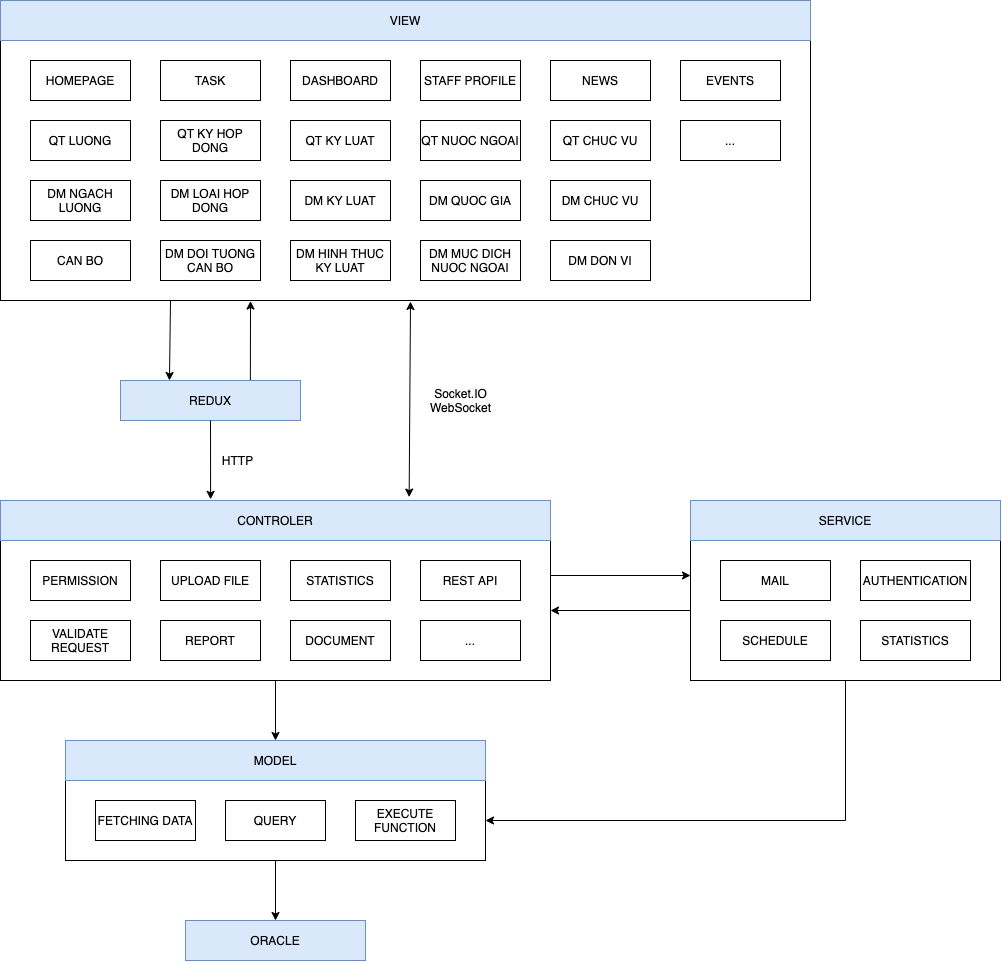
\includegraphics[width=15cm]{img/MVCInTchc.png}
  \captionof{figure}{Kiến trúc tổng thể của hệ thống}
\end{center}

\section{Nguyên tắc thiết kế hệ thống}
\indent Với một hệ thống khá phức tạp như trên cần phải có những nguyên tắc thiết kế chung
\subsection{Cấu trúc cây thư mục của mã nguồn}
Việc cần làm đầu tiên và quan trọng nhất là tổ chức files và các thư mục. Với một thiết kế tốt thì khi làm việc chung giữa nhiều người sẽ ít bị đụng độ. Nhóm lựa chọn cách chia mỗi thành phần của trang ra từng module tách biệt với nhau, thuận lợi cho việc mở rộng và bảo trì, bảo dưỡng.\\

Dựa vào kiến trúc hệ thống mà nhóm đã thiết kế ở trên, nhóm đã chọn cấu trúc mã nguồn như sau:
\begin{center}
  \captionsetup{type=figure}
  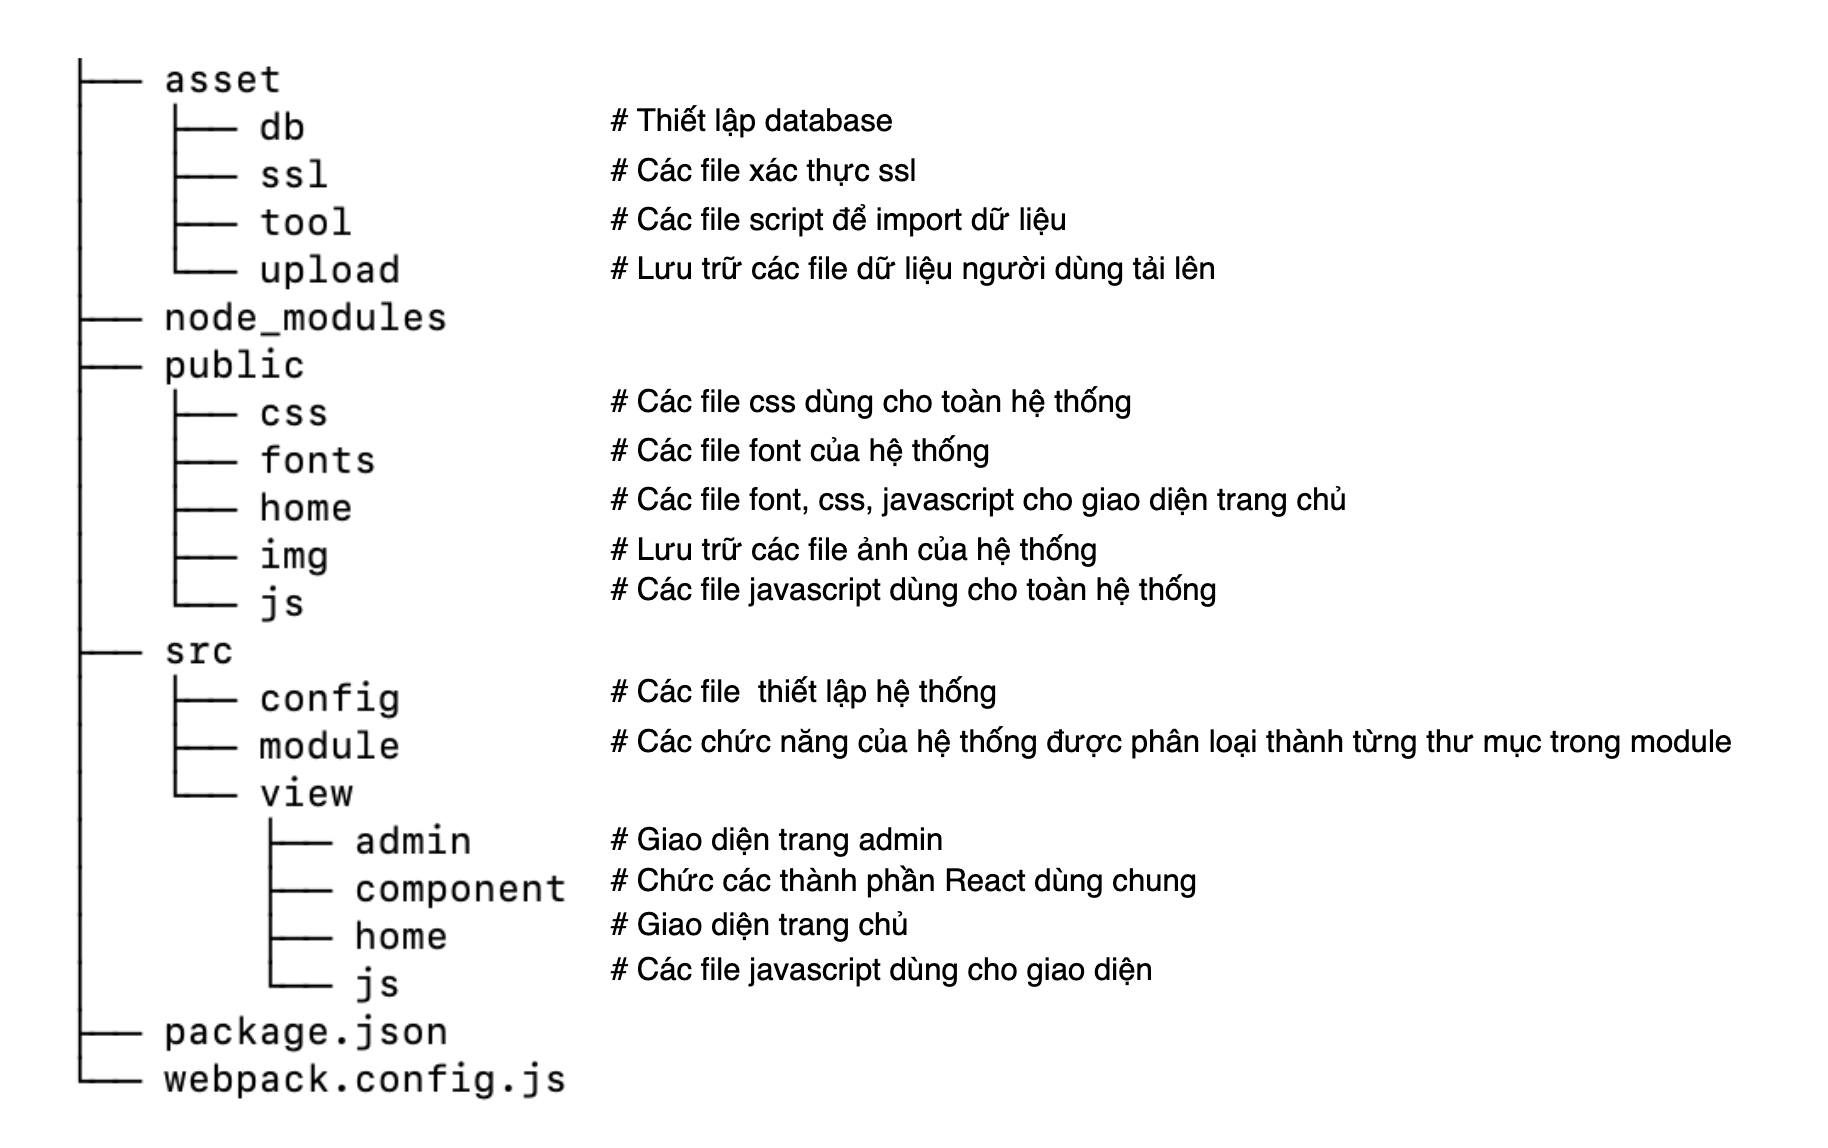
\includegraphics[width=15cm]{img/tree.png}
  \captionof{figure}{Cây thư mục của hệ thống}
\end{center}
\section{Thiết kế đối tượng người dùng}
\subsection{Danh sách đối tượng người dùng}
\begin{center}
  \captionsetup{type=figure}
  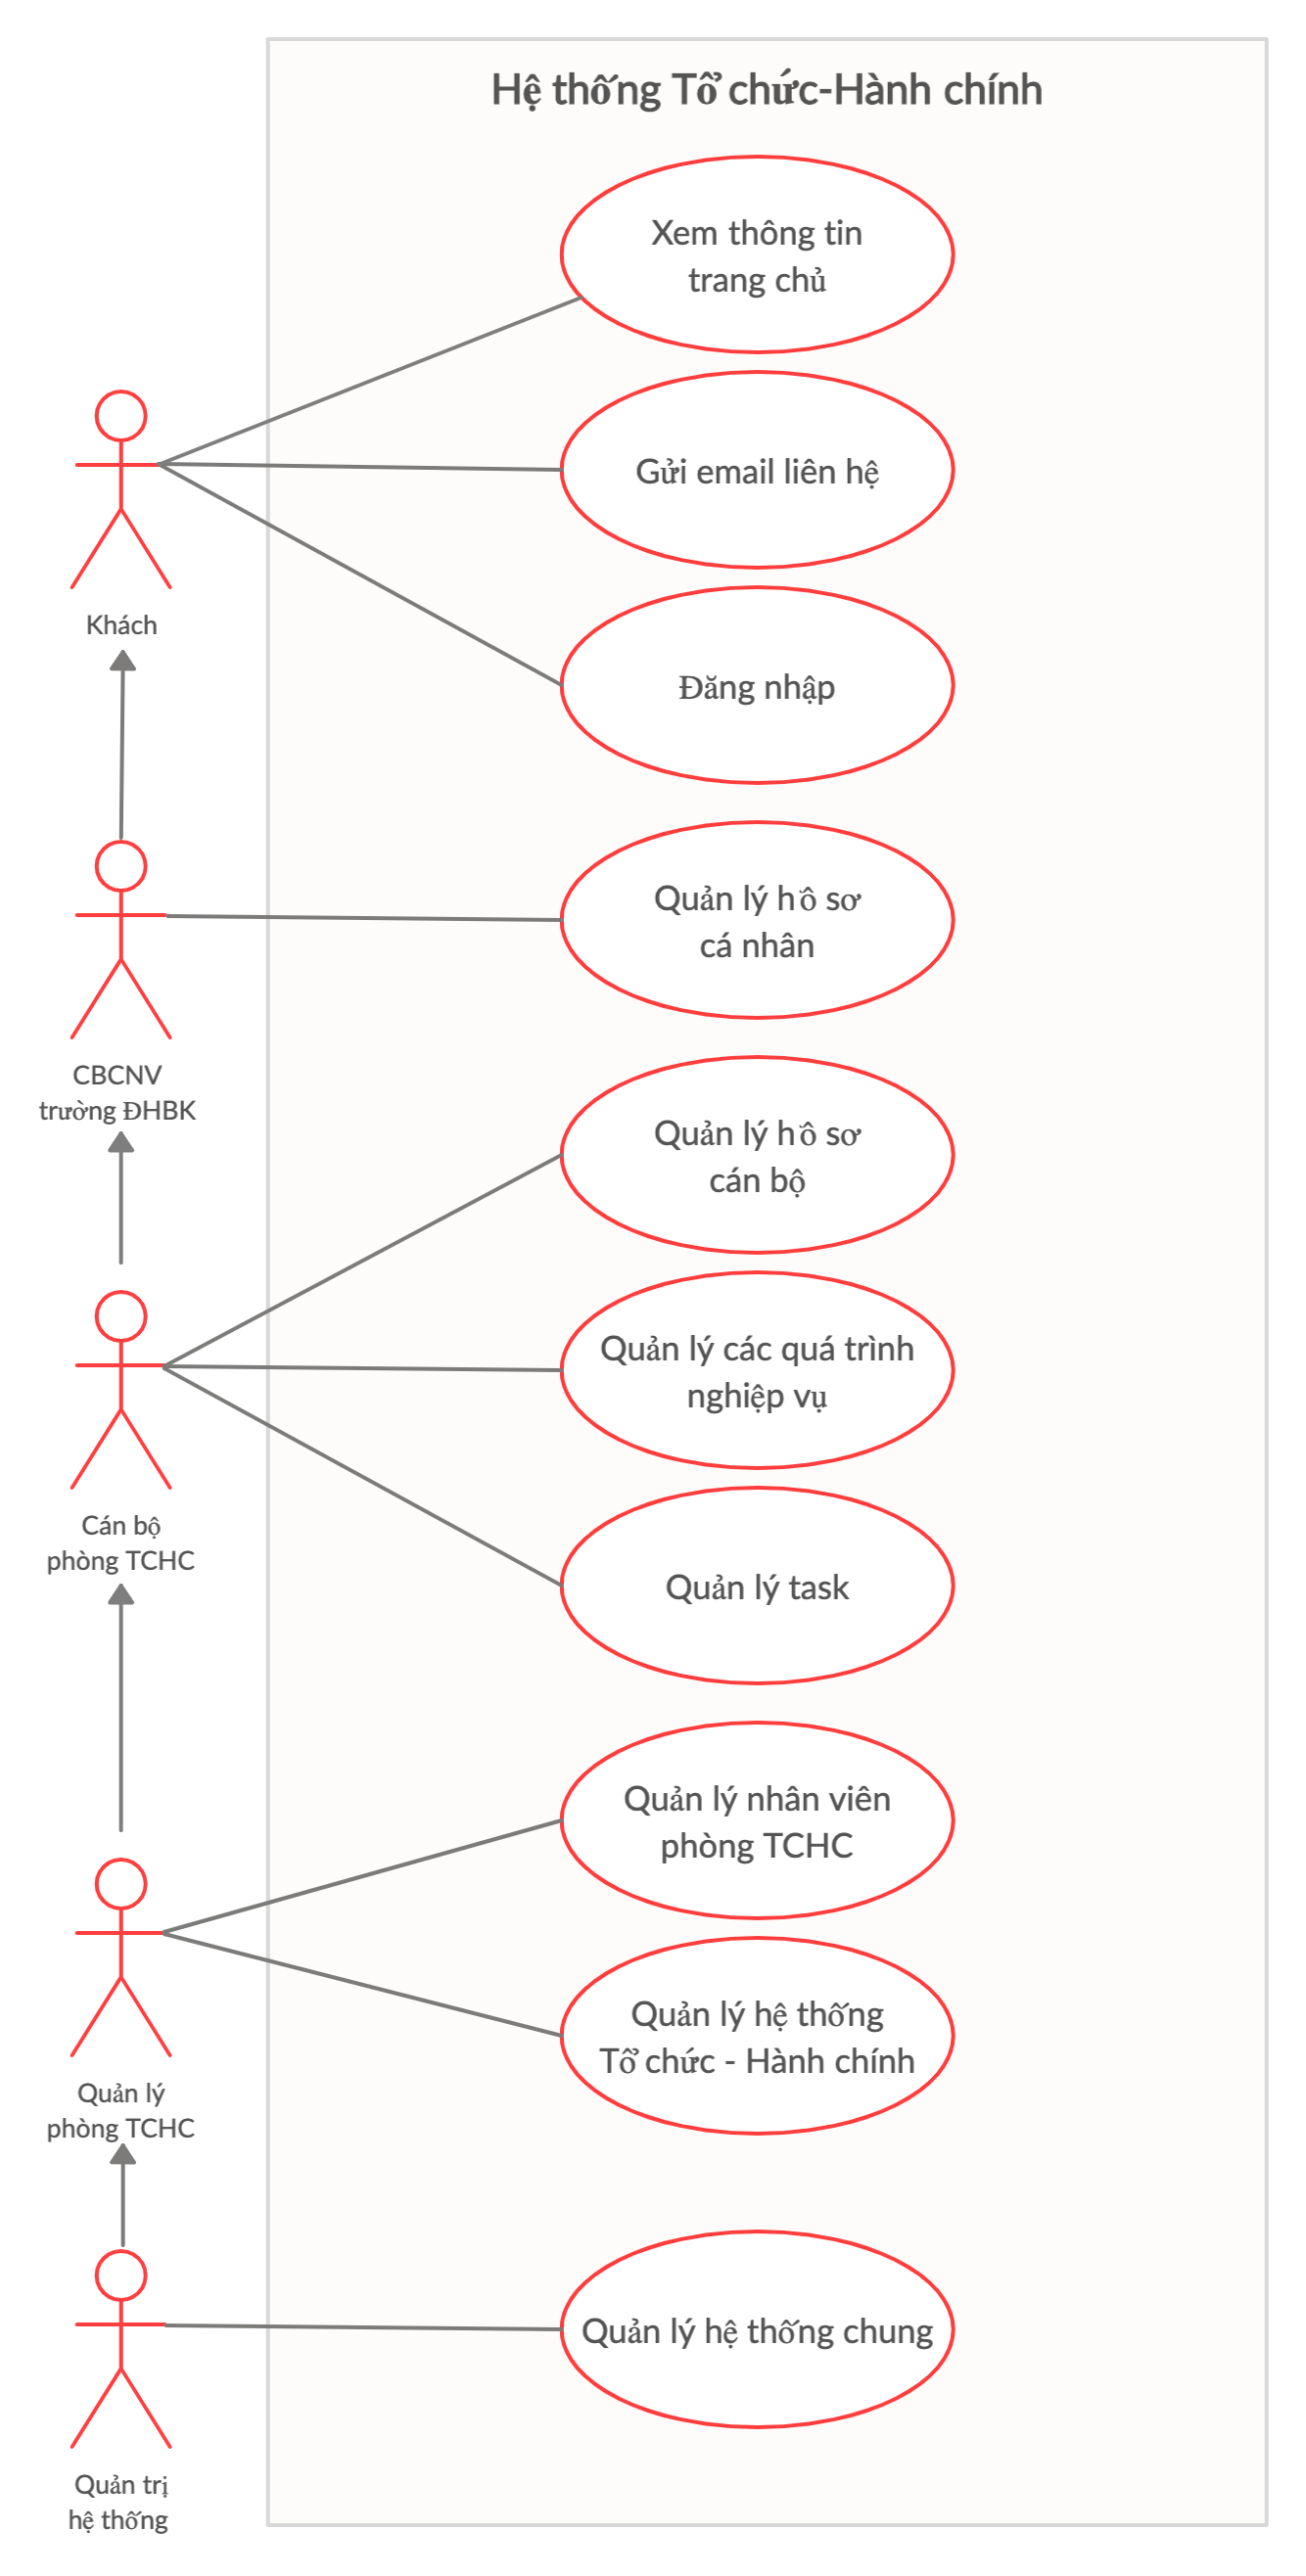
\includegraphics[width=11cm]{img/usecase/rootUsecase.png}
  \captionof{figure}{Lược đồ Usecase các đối tượng của hệ thống }
\end{center}
\begin{table}[H]
    \centering
	\begin{tabular}{|p{1cm}|p{4cm}|p{10cm}|}
    \hline
    \textbf{STT}&\textbf{Người dùng}&\textbf{Đặc tả}\\
    \hline
    1&Khách&Là những người dùng chưa đăng nhập, bao gồm tất cả các đối tượng như cán bộ,  công nhân viên nhà trường, sinh viên, cựu sinh viên, phụ huynh, đơn vị, doanh nghiệp là đối tác của nhà trường,...
    
    Khách có chức năng xem thông tin, tin tức, sự kiện của nhà trường, gửi email liên hệ, và đăng nhập.\\
    \hline
	2&Cán bộ, công nhân viên nhà trường&Người dùng với mục đích quản lý được thông tin, các quá trình nghiệp vụ của bản thân.\\
	\hline
    3&Cán bộ phòng Tổ chức - Hành chính&Là những cán bộ thuộc phòng Tổ chức - Hành chính. Họ có chức năng quản lý thông tin của các cán bộ, quản lý thông tin các quá trình nghiệp vụ của nhà trường.\\
    \hline
    4&Quản lý phòng Tổ chức - Hành chính (Trưởng phòng, phó phòng) &Chức năng chính là quản lý hệ thống và công việc của các cán bộ thuộc phòng Tổ chức - Hành chính. \\
	\hline
    5&Quản trị hệ thống&Là những người tạo ra hệ thống ban đầu, có các chức năng hỗ trợ tạo ra các cấu hình cho hệ thống, bao gồm các thao tác như: cấu hình các thông tin chung của phòng Tổ chức-Hành chính, cấu hình về giao diện, quản lý tài khoản người dùng\\
	\hline
\end{tabular}
\caption{Danh sách đối tượng người dùng của hệ thống}
\end{table}
\subsection{Đối tượng: Khách}
\textbf{Lược đồ Usecase đối tượng khách}
\begin{center}
  \captionsetup{type=figure}
  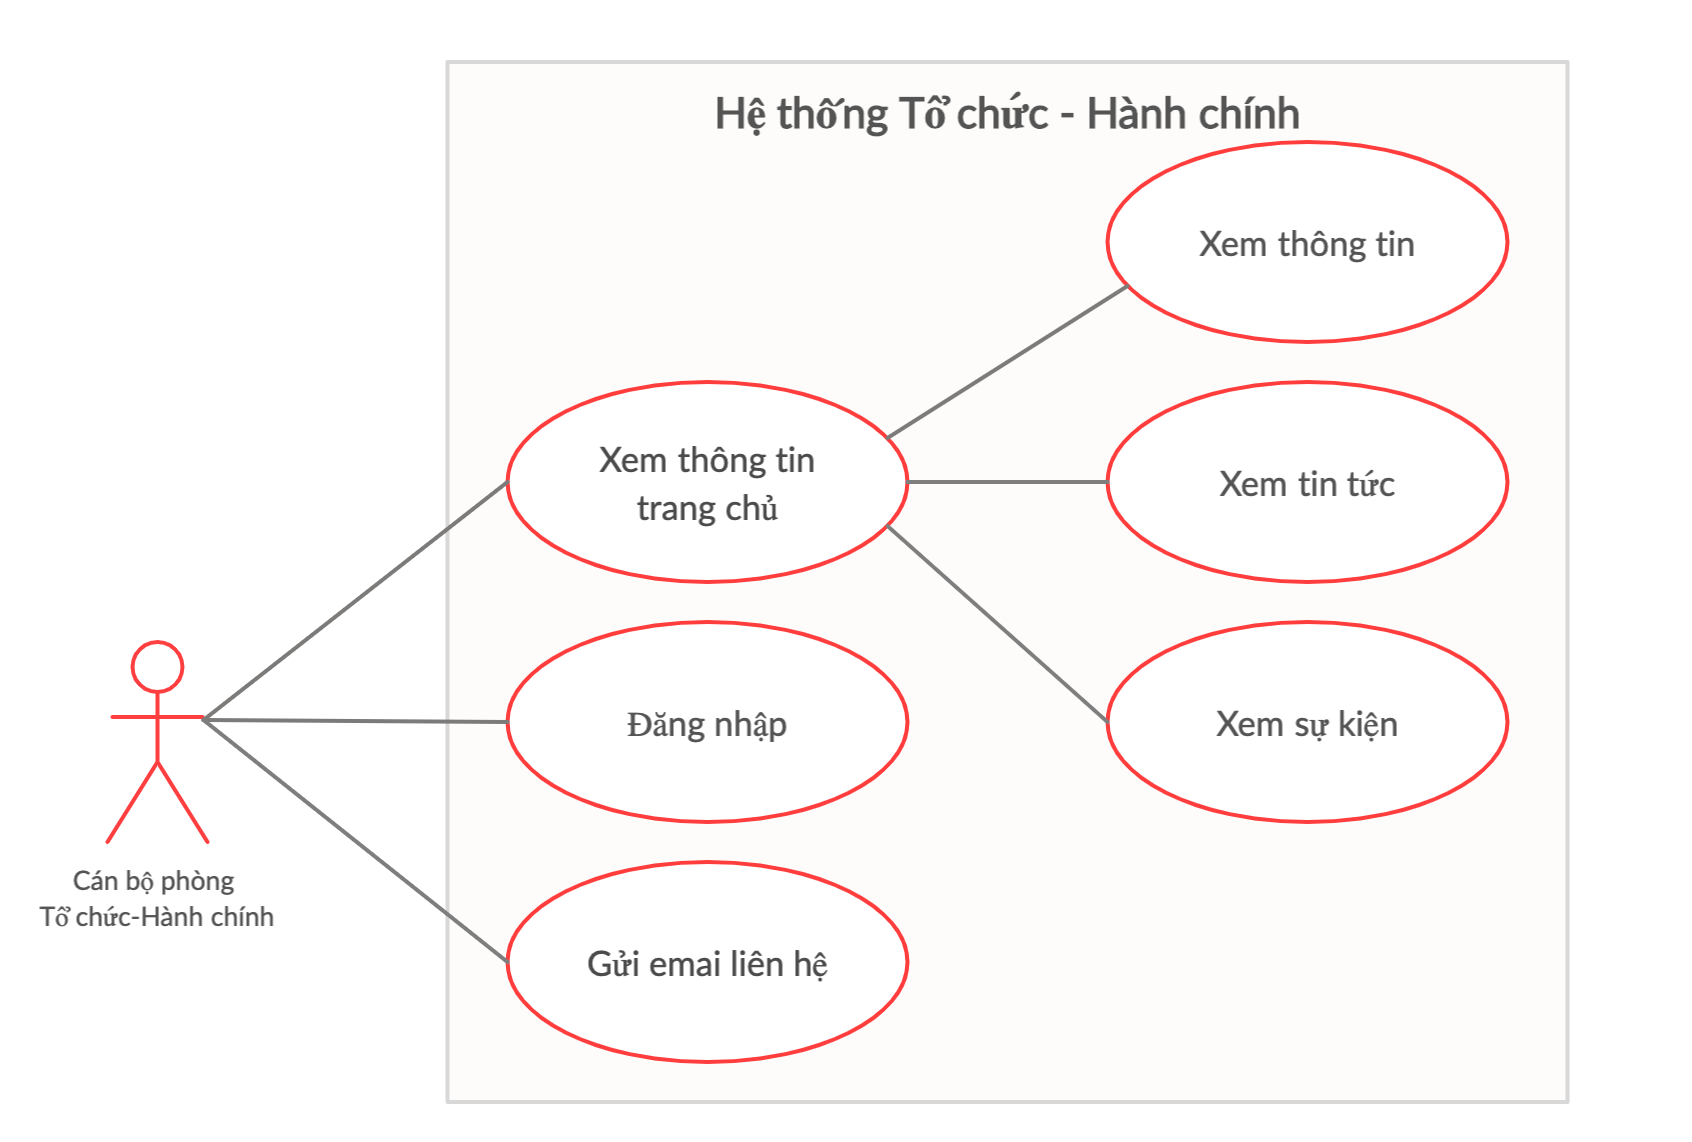
\includegraphics[width=15cm]{img/usecase/guest.png}
  \captionof{figure}{Lược đồ usecase của đối tượng khách}
\end{center}

Khách là những người dùng chưa đăng nhập, bao gồm tất cả các đối tượng như cán bộ,  công nhân viên nhà trường, sinh viên, cựu sinh viên, phụ huynh, đơn vị, doanh nghiệp là đối tác của nhà trường,...
 
 Đối tượng khách có thể truy cập trang chủ để xem các thông tin chung, thông tin liên hệ, xem các tin tức và sự kiện. Khi có nhu cầu liên hệ với nhà trường, khách có thể vào mục liên hệ để gửi email đến nhà trường.
 
 Khi khách là cán bộ công nhân viên trường Đại học Bách Khoa Tp.HCM, khách có thể đăng nhập bằng tài khoản email nhà trường cung cấp để sử dụng hệ thống với các vai trò cán bộ nhà trường.

\subsection{Đối tượng: Cán bộ công nhân viên nhà trường}
\textbf{Lược đồ Usecase đối tượng cán bộ của trường}
\begin{center}
  \captionsetup{type=figure}
  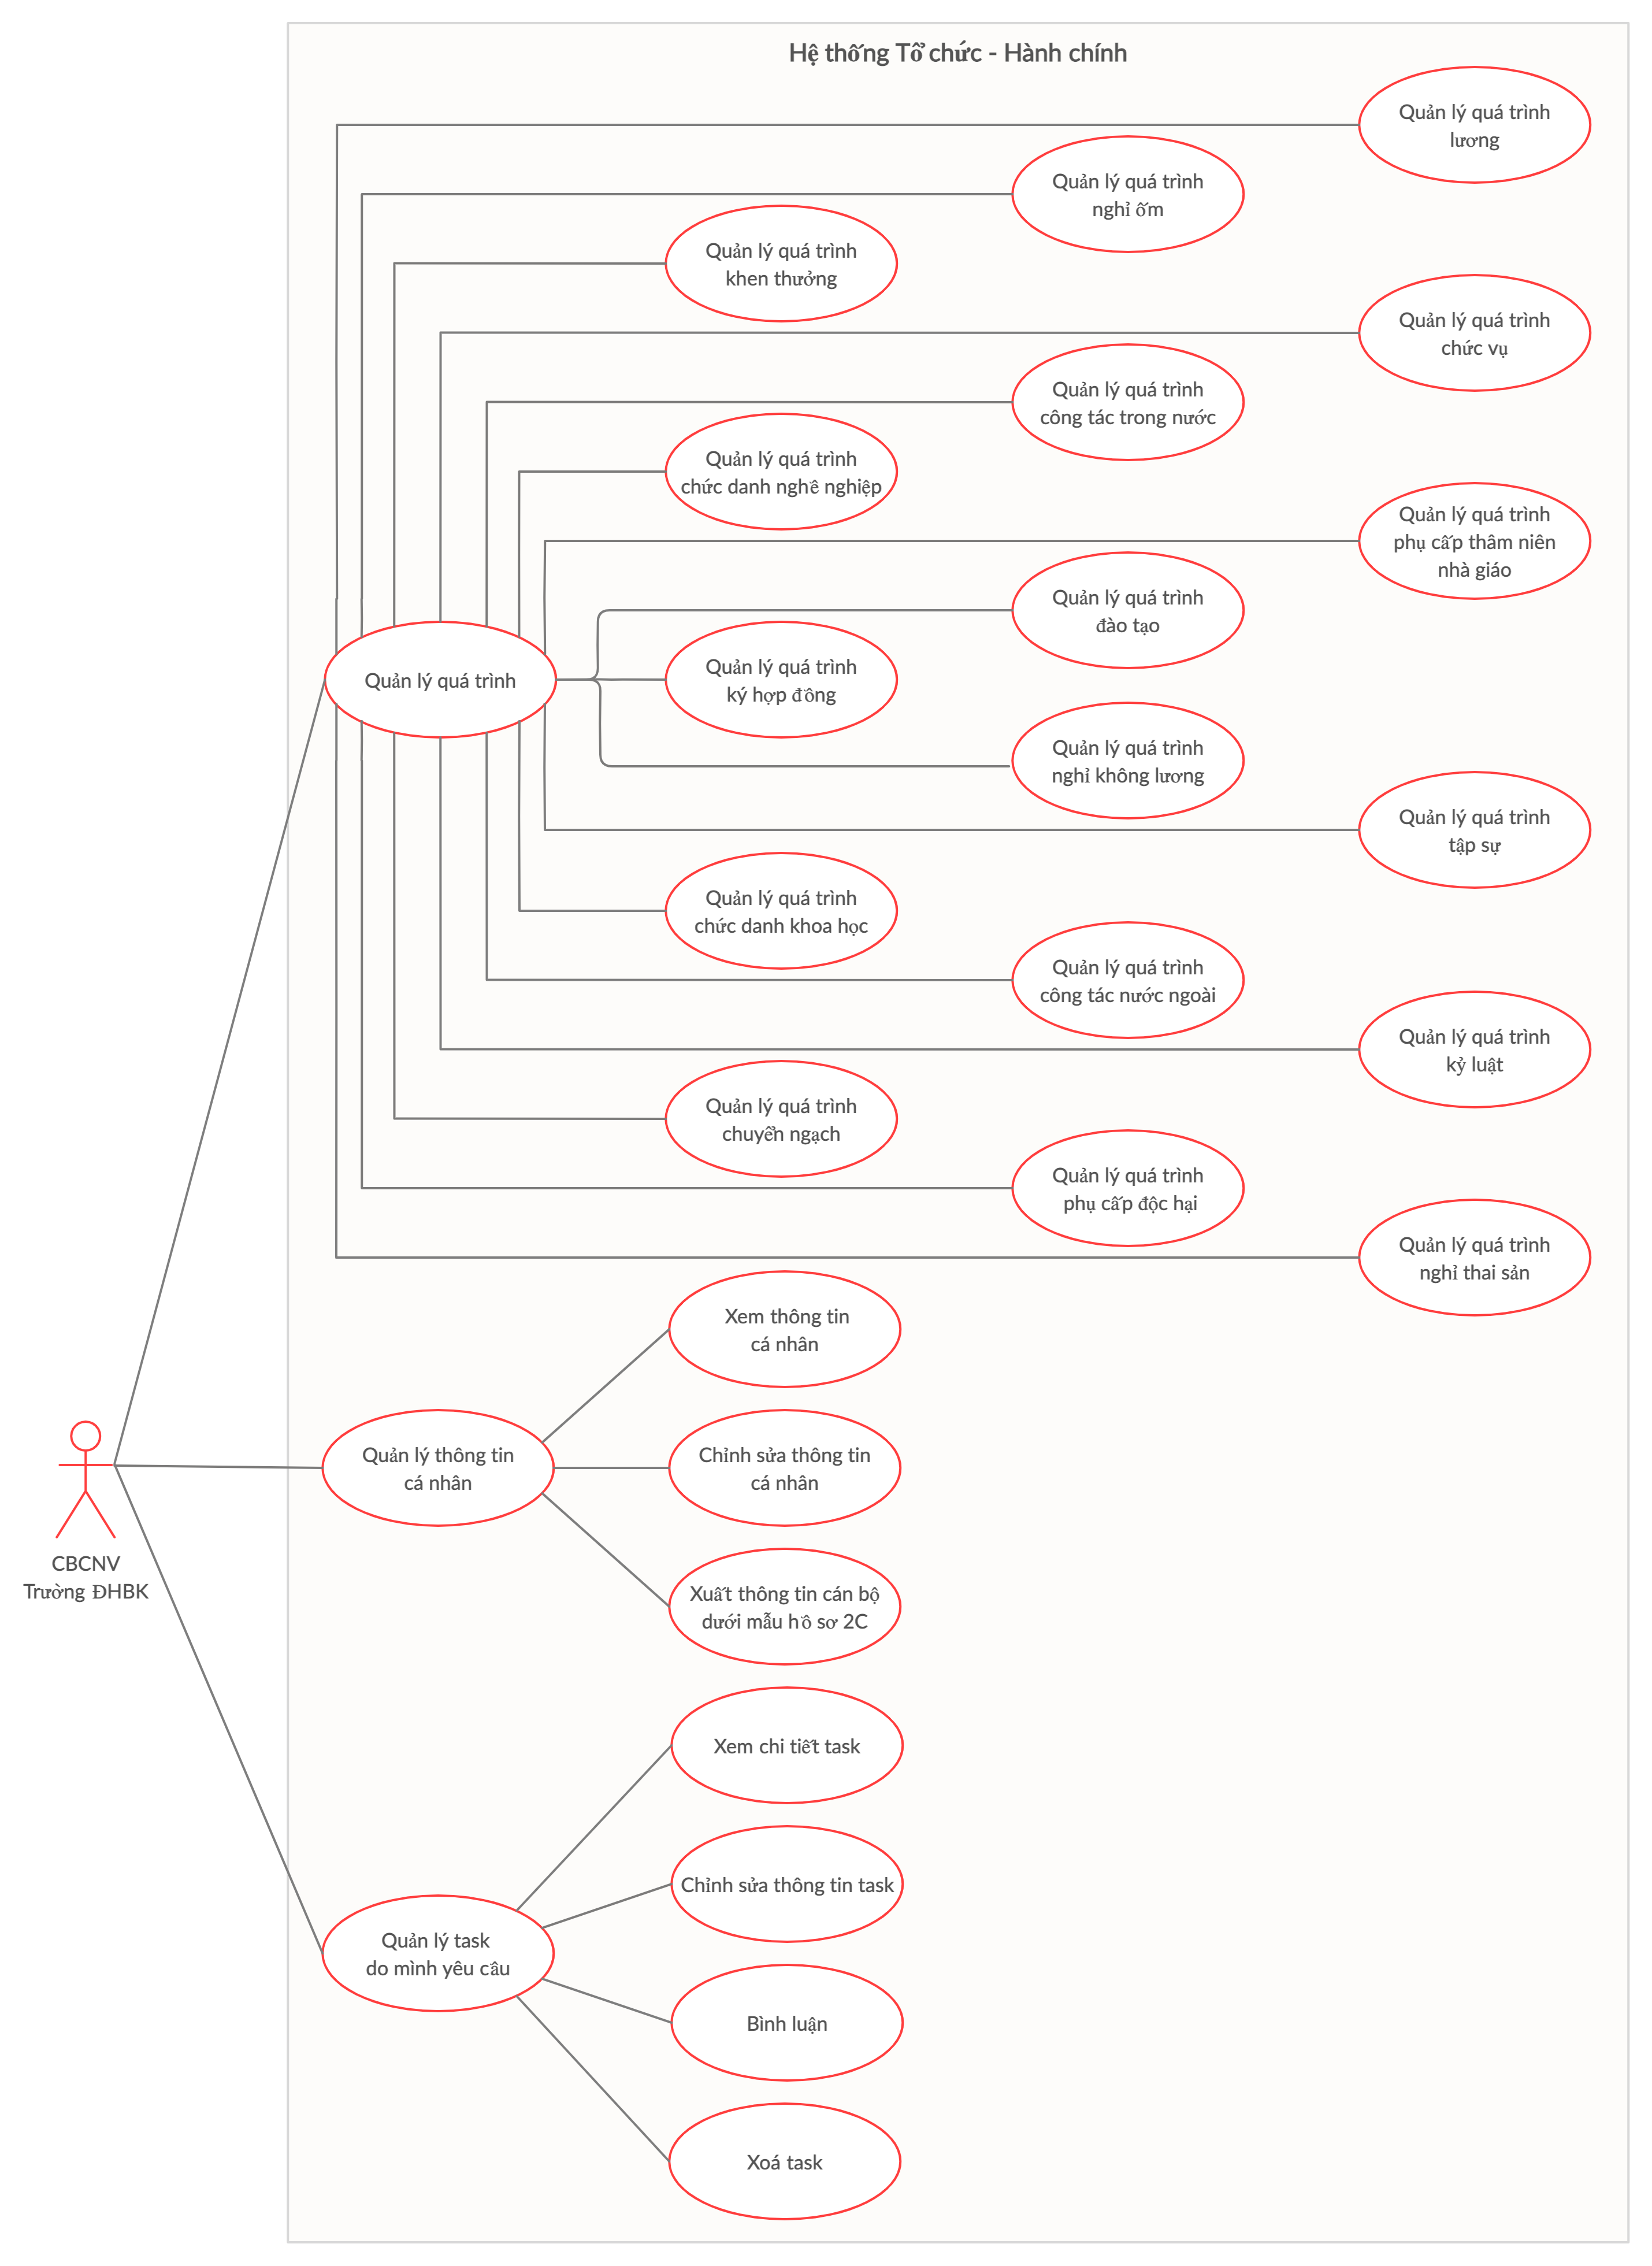
\includegraphics[width=15cm]{img/usecase/userUsecase.png}
  \captionof{figure}{Lược đồ Usecase đối tượng cán bộ của trường}
\end{center}

Đối với người dùng là cán bộ của trường, sau khi đăng nhập sẽ có chức năng quản lý thông tin của cá nhân, quản lý các quá trình nghiệp vụ của bản thân.

Quản lý thông tin cá nhân bao gồm xem thông tin, sửa đổi và xuất thông tin theo mẫu sơ yếu lý lịch cán bộ, công chức (Mẫu 2C-BNV/2008).

Cán bộ có thể xem thông tin các quá trình nghiệp vụ của bản thân như quá trình lương, quá trình nghỉ ốm, nghỉ không lương, nghỉ thai sản,... 

Khi muốn tạo mới, sửa đổi hoặc xoá quá trình, cán bộ công nhân viên nhà trường có thể tạo yêu cầu tương ứng để cán bộ phòng Tổ chức - Hành chính xem xét và duyệt yêu cầu.

\subsection{Đối tượng: Cán bộ phòng Tổ chức - Hành chính}
\textbf{Lược đồ Usecase đối tượng cán bộ phòng Tổ chức - Hành chính}
\begin{center}
  \captionsetup{type=figure}
  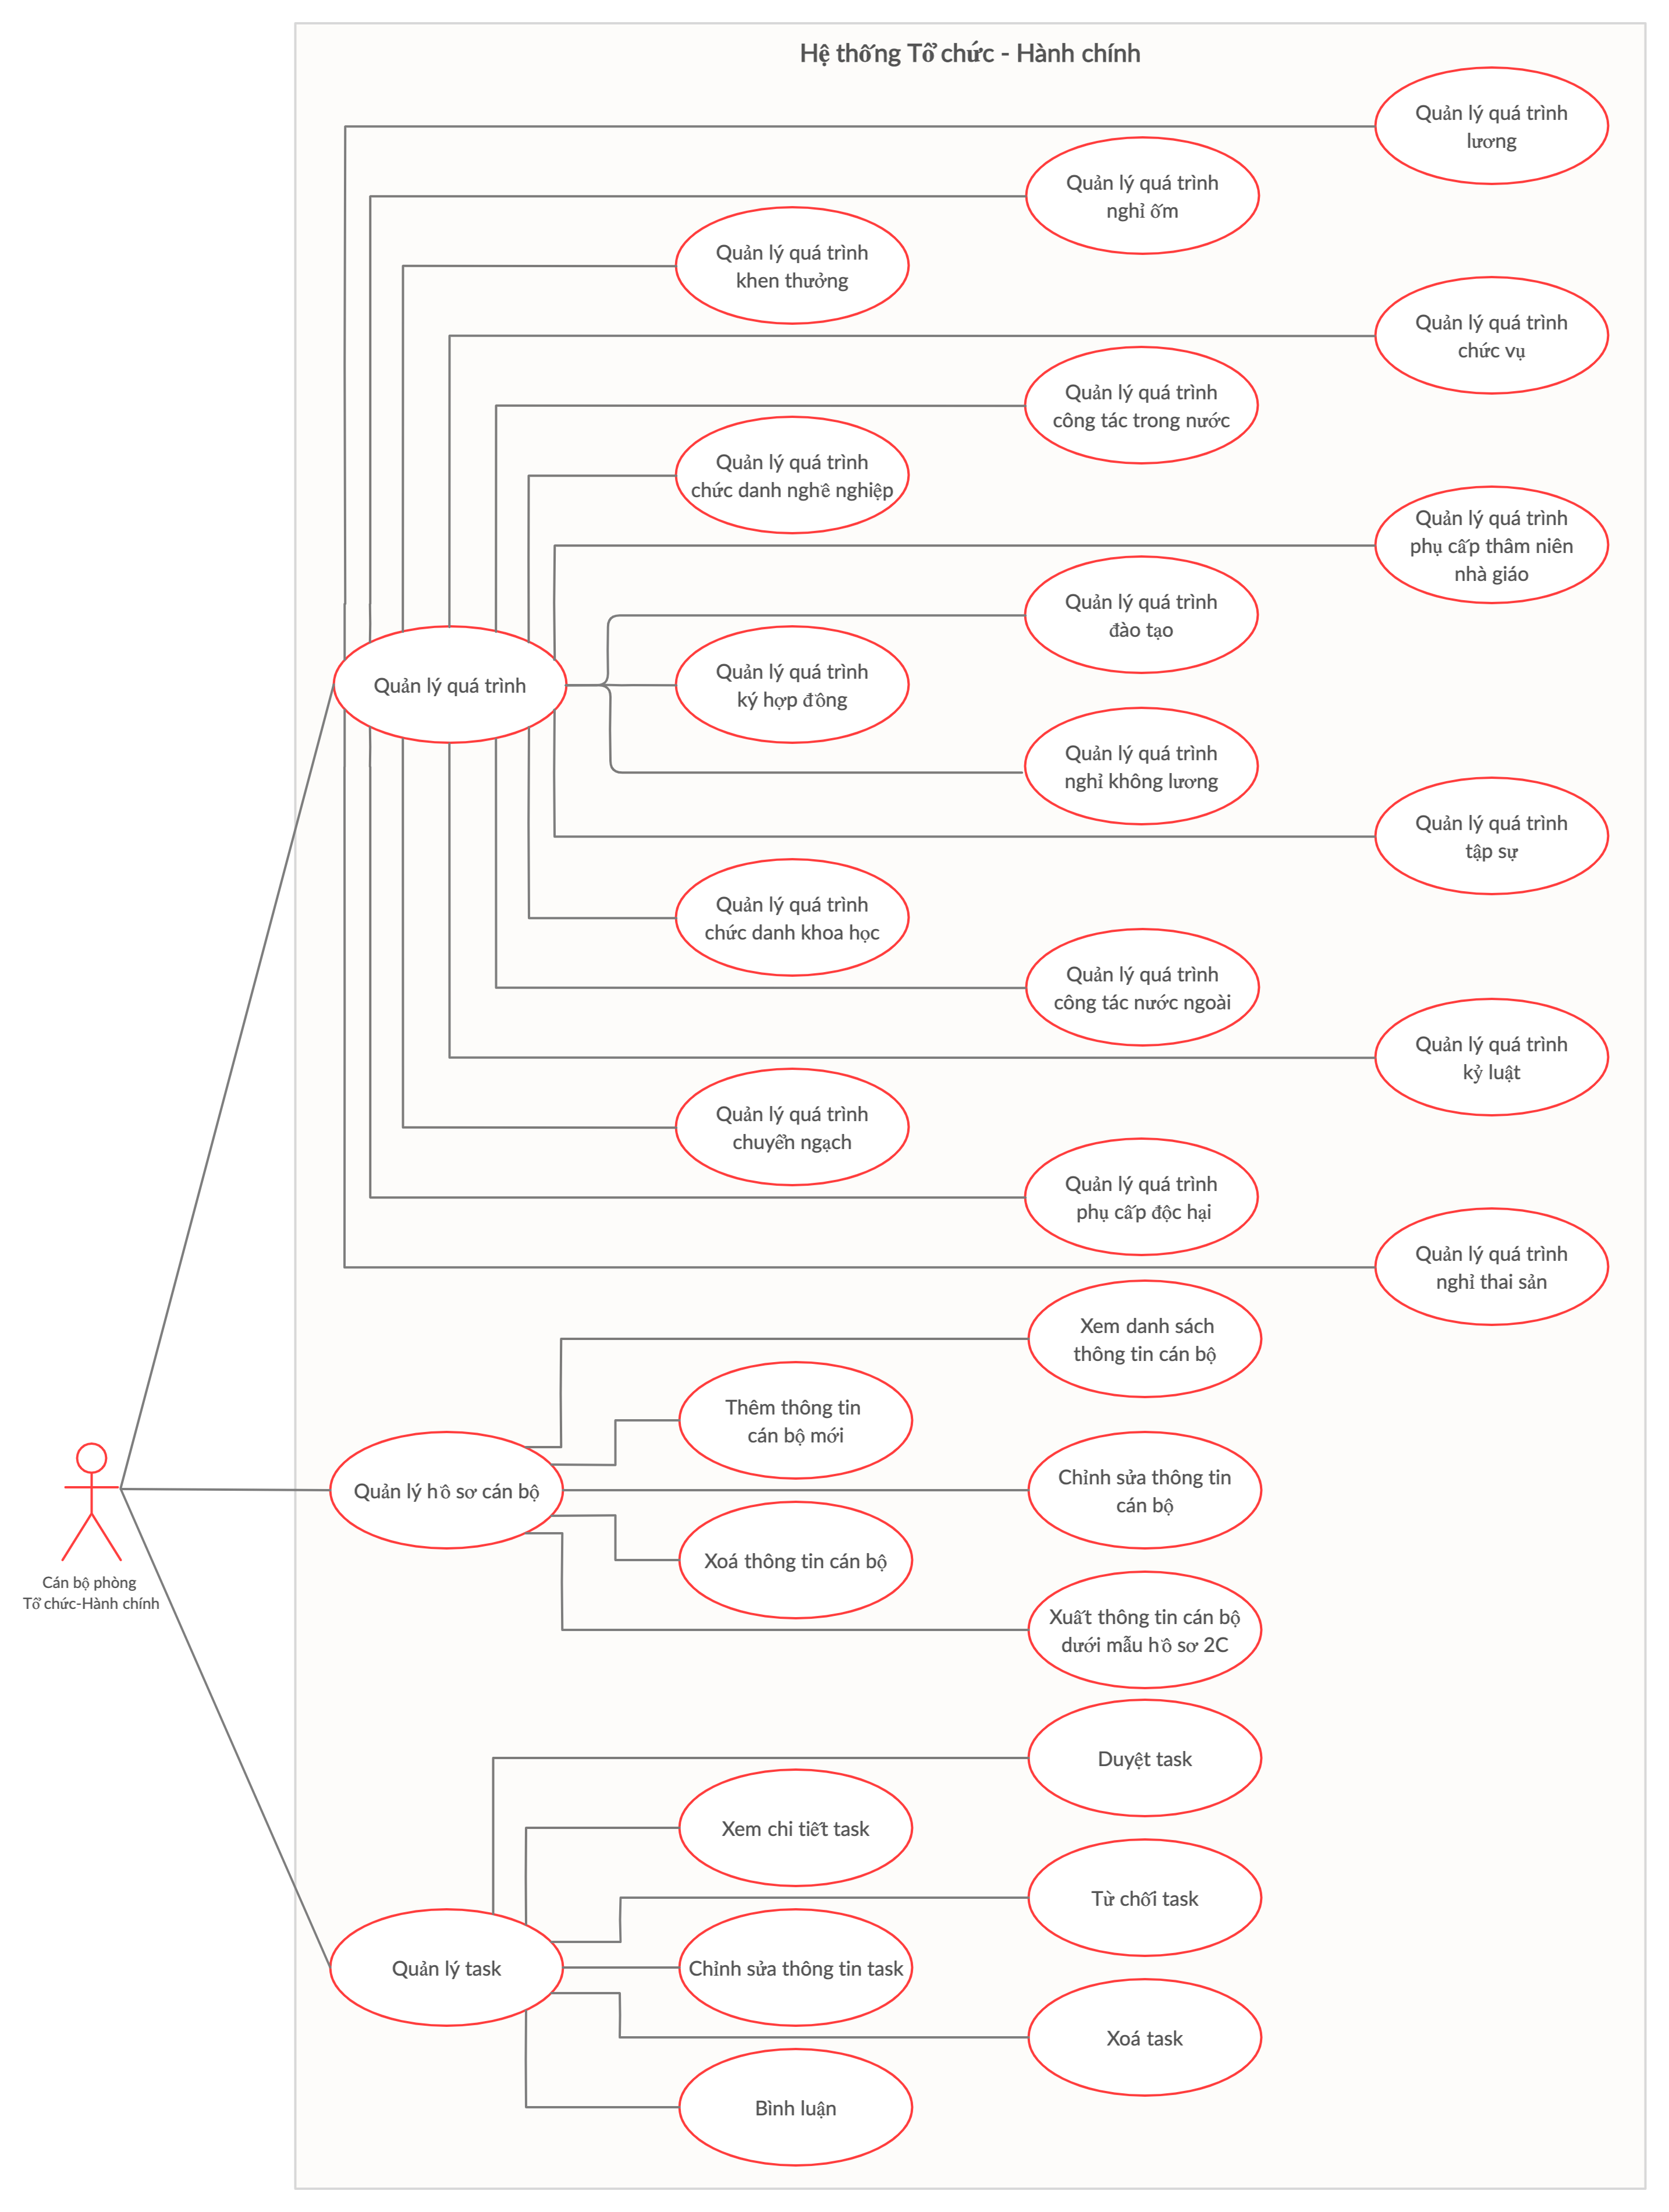
\includegraphics[width=15cm]{img/usecase/nhanVienTCHC.png}
  \captionof{figure}{Lược đồ Usecase đối tượng cán bộ phòng Tổ chức - Hành chính}
\end{center}

Sau khi đăng nhập vào hệ thống, người dùng là cán bộ phòng Tổ chức - Hành chính sẽ có các nhóm chức năng sau: quản lý cán bộ, quản lý các quá trình nghiệp vụ và các yêu cầu của của người dùng.

Chức năng quản lý cán bộ bao gồm xem danh sách toàn bộ cán bộ nhà trường, tạo mới, sửa đổi và xoá cán bộ. Ngoài ra còn có chức năng xuất danh sách cán bộ dưới dạng excel, xuất hồ sơ lý lịch theo mẫu 2C.

Chức năng quản lý các quá trình nghiệp vụ bao gồm xem danh sách các quá trình như quá trình công tác trong nước, quá trình công tác nước ngoài, quá trình lương,... Tạo mới quá trình, chỉnh sửa thông tin quá trình và xoá quá trình.

Cán bộ phòng Tổ chức - Hành chính còn có nhiệm vụ quản lý các yêu cầu của các cán bộ công nhân viên nhà trường, xem xét, chỉnh sửa, bình luận, từ chối và duyệt yêu cầu.

\subsection{Đối tượng: Quản lý phòng Tổ chức - Hành chính}
\textbf{Lược đồ Usecase đối tượng quản lý phòng Tổ chức - Hành chính}
\begin{center}
  \captionsetup{type=figure}
  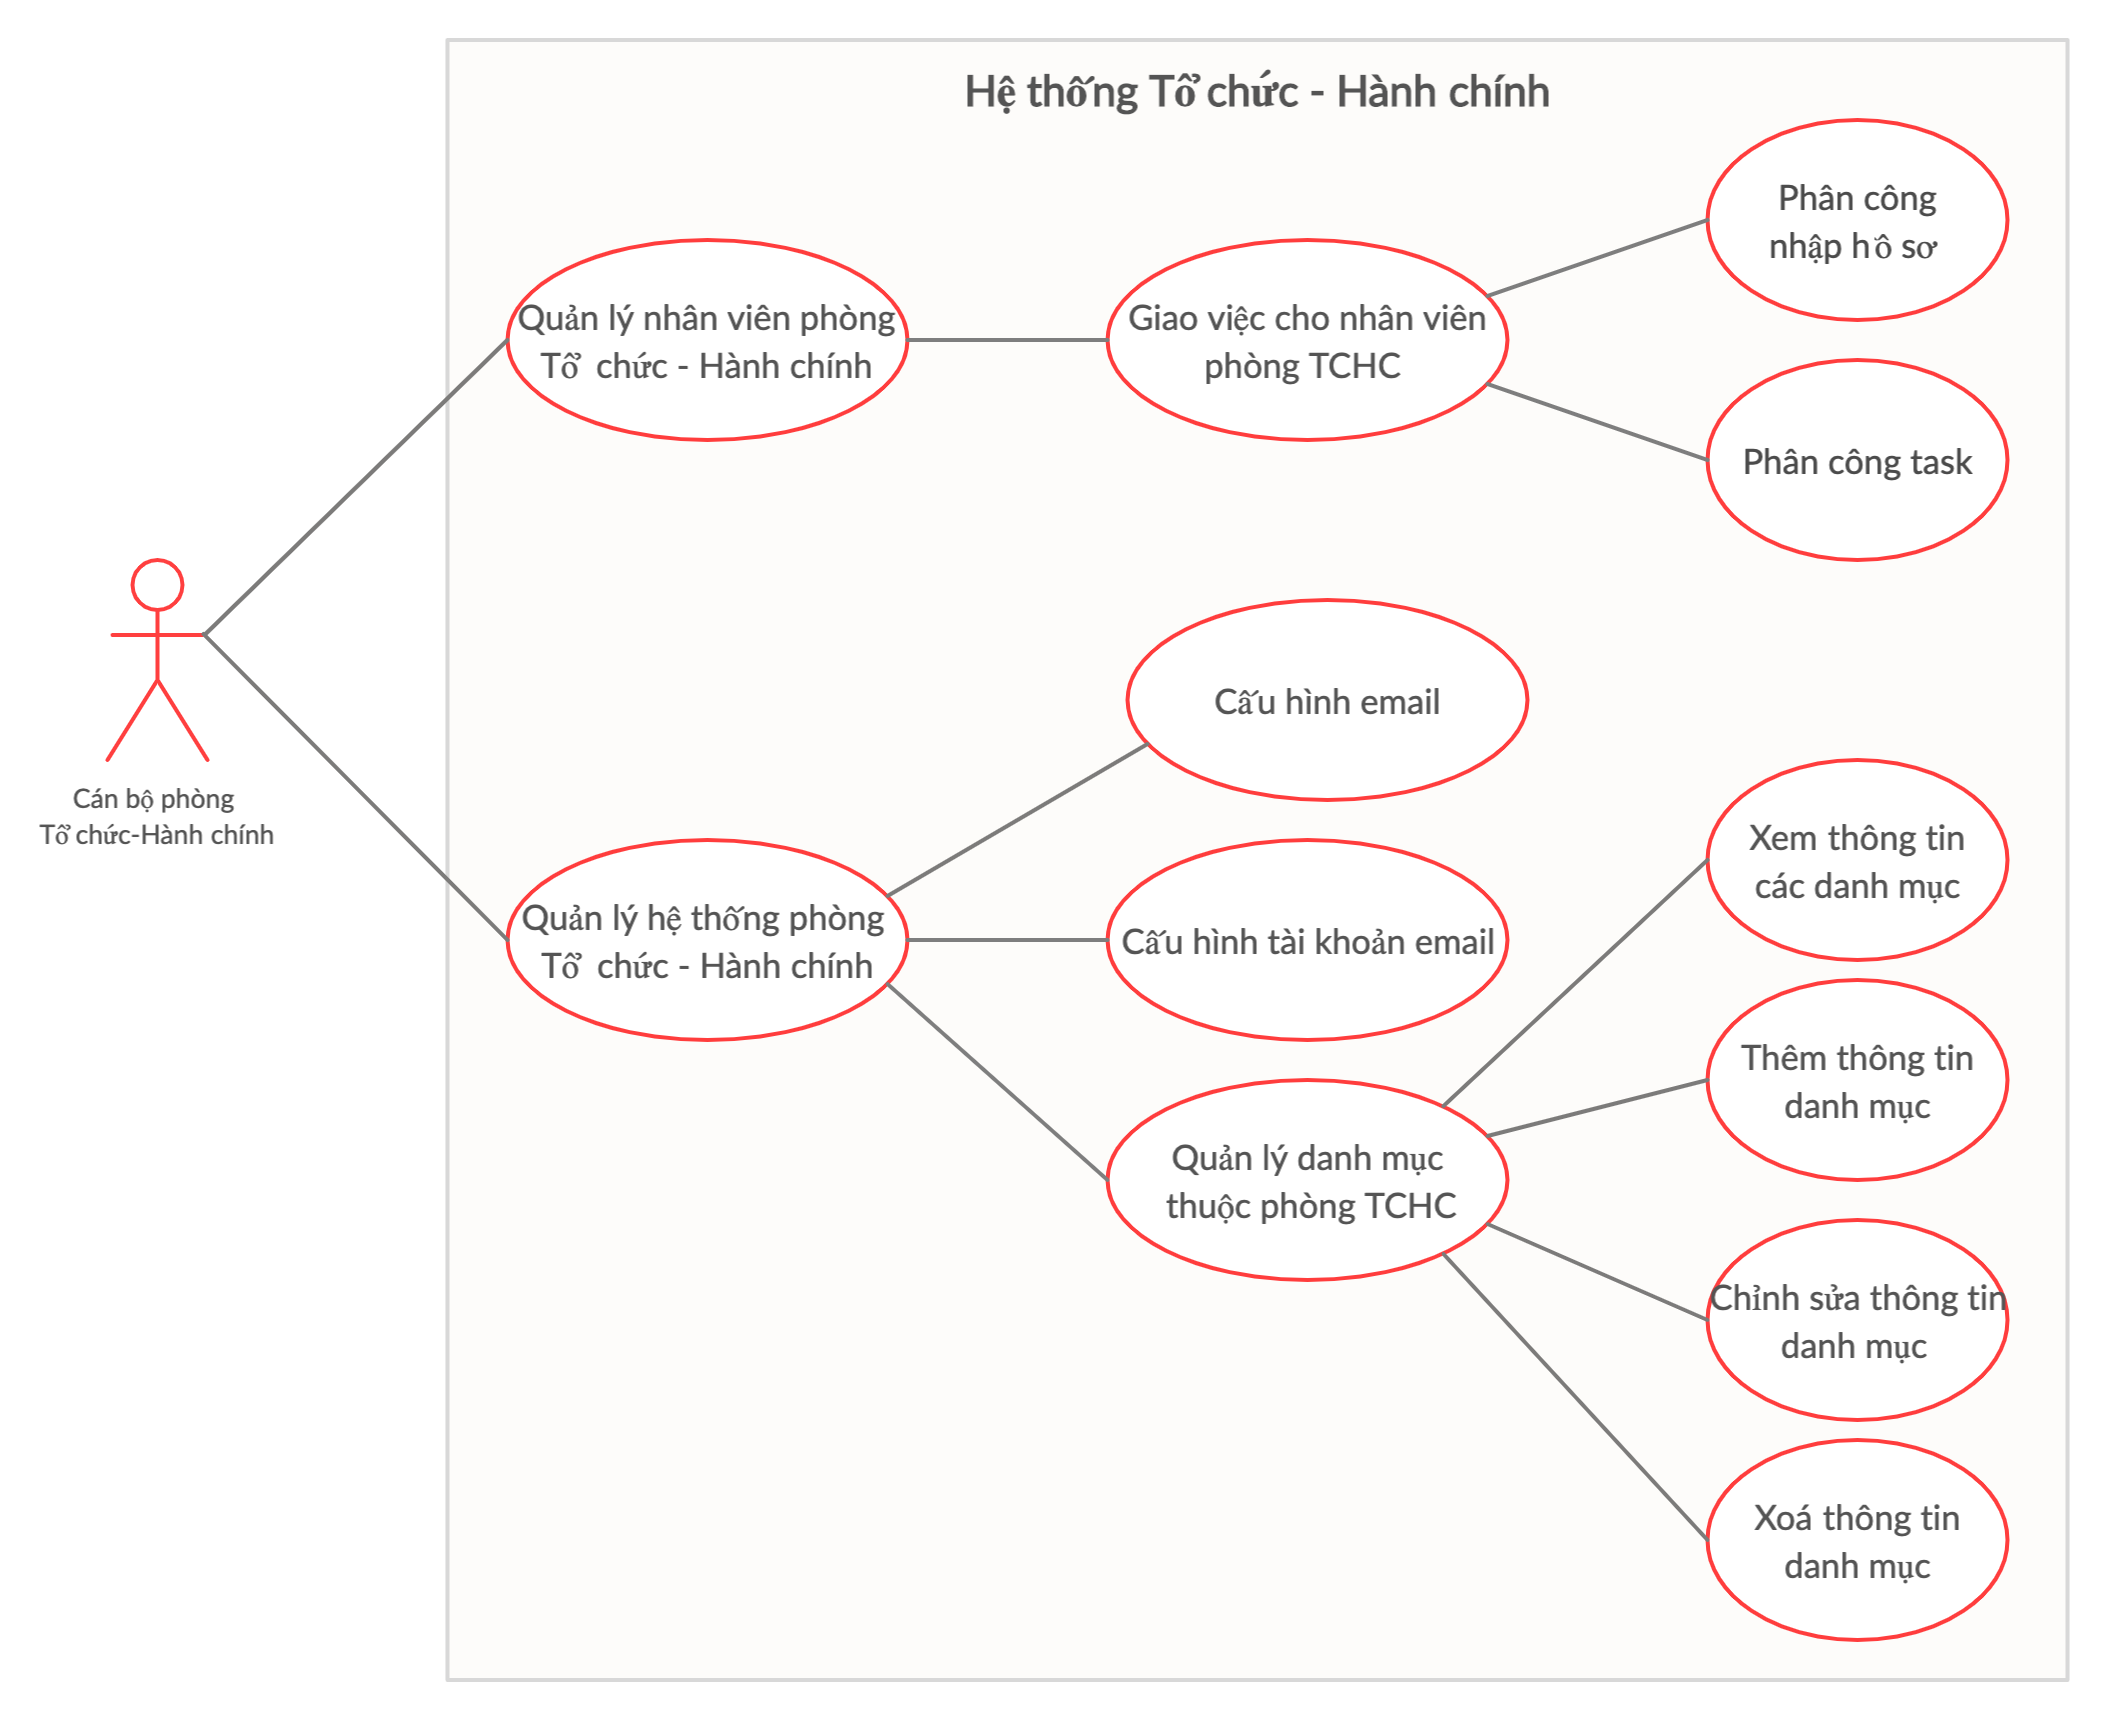
\includegraphics[width=15cm]{img/usecase/quanLyPhong.png}
  \captionof{figure}{Lược đồ Usecase cho đối tượng quản lý phòng Tổ chức - Hành chính}
\end{center}
Quản lý phòng Tổ chức - Hành chính sau khi đăng nhập sẽ có tất cả các nhóm chức năng như trên của cán bộ của phòng Tổ chức - Hành chính và có thêm chức năng quản trị các danh mục, thông tin thuộc phòng Tổ chức - Hành chính.

Bên cạnh đó, quản lý phòng còn có nhiệm vụ phân công công việc cho nhân viên như phân công nhập hồ sơ, phân công duyệt yêu cầu.

\subsection{Đối tượng: Quản trị hệ thống}
\textbf{Lược đồ Usecase đối tượngq quản trị hệ thống}
\begin{center}
  \captionsetup{type=figure}
  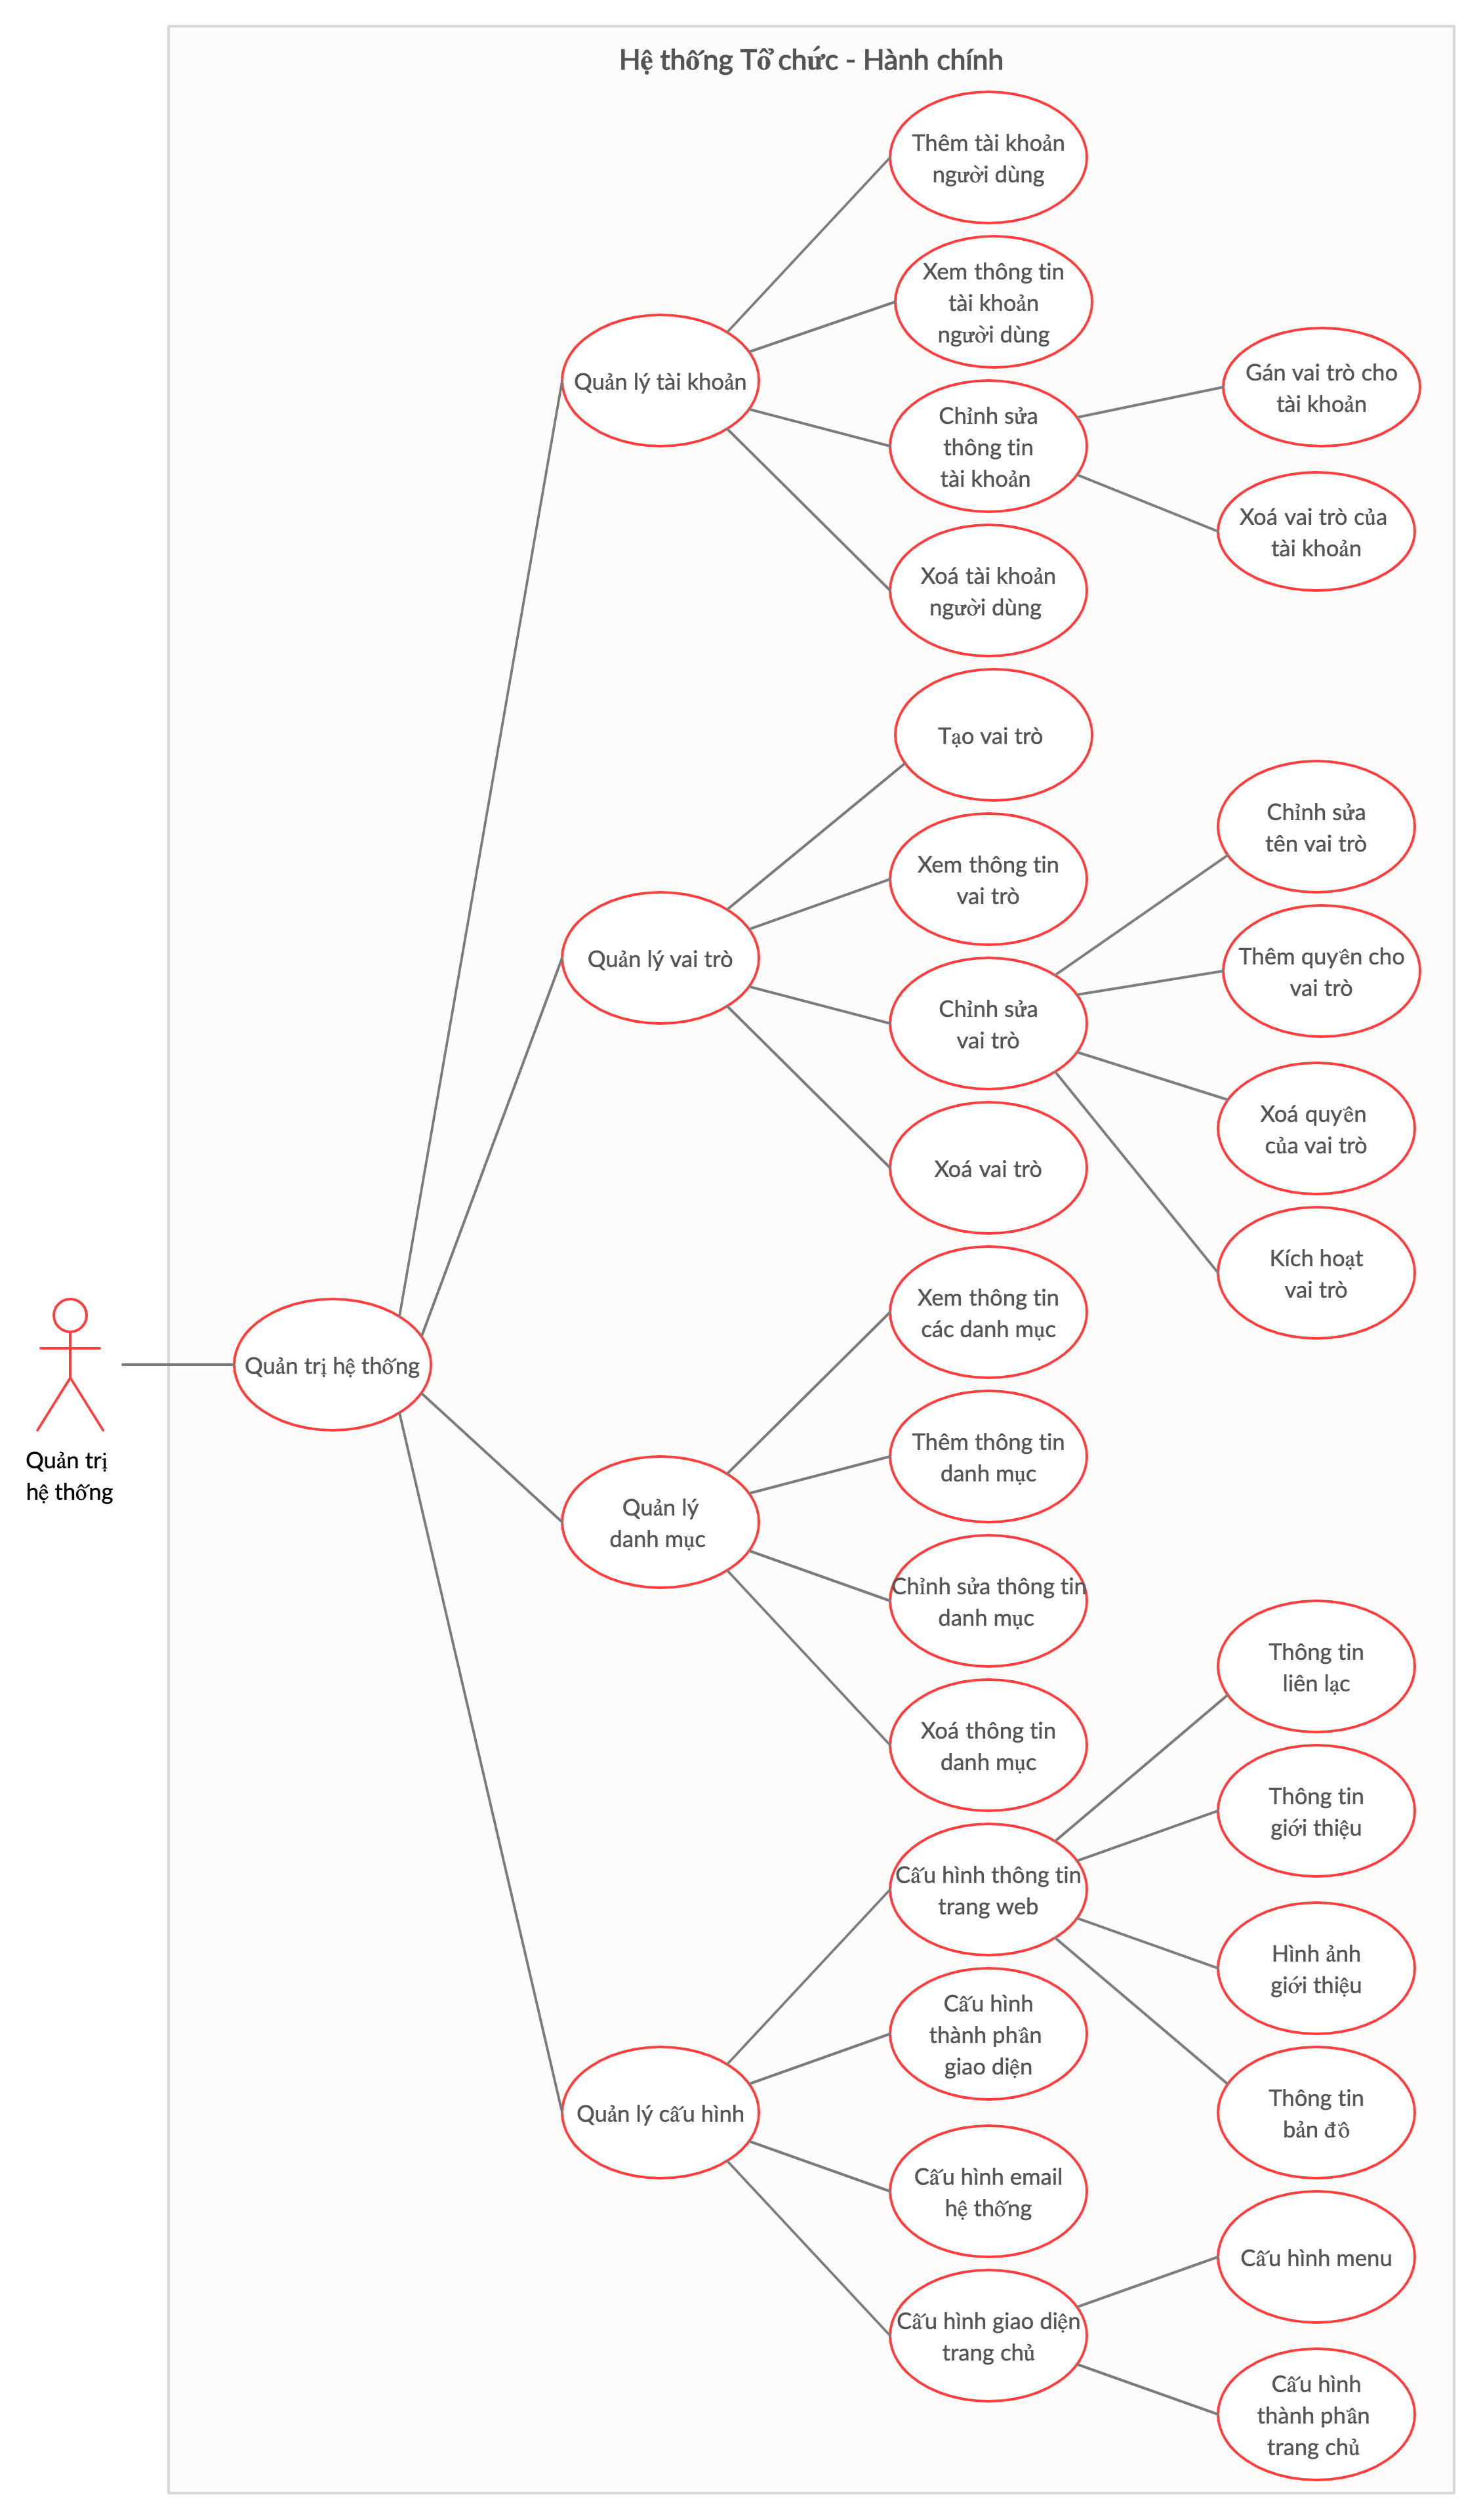
\includegraphics[width=13cm]{img/usecase/admin.png}
  \captionof{figure}{Lược đồ usecase của đối tượng quản trị hệ thống}
\end{center}

\indent Đối với đối tượng là quản trị hệ thống, sau khi xác thực thành công sẽ có những nhóm chức năng: quản lý tài khoản, quản lý vai trò, quản lý danh mục và quản lý cấu hình. Với mỗi nhóm chức năng sẽ có những chức năng tương ứng sau:

\begin{itemize}
    \item Nhóm quản lý tài khoản bao gồm các chức năng:
        \subitem - Xem thông tin các tài khoản.
        \subitem - Tạo mới tài khoản.
        \subitem - Xoá tài khoản người dùng.
        \subitem - Chỉnh sửa thông tin tài khoản.
        \subitem - Thêm và xoá vai trò cho tài khoản.
    \item Nhóm quản lý vai trò bao gồm các chức năng:
        \subitem - Xem danh sách các vai trò.
        \subitem - Tạo mới và xoá vai trò.
        \subitem - Kích hoạt vai trò.
        \subitem - Thêm và xoá quyền cho vai trò.
    \item Chức năng quản lý danh mục là chức năng xây dựng và sửa đổi thông tin những danh mục mặc định phục vụ cho việc nhập và lữu trữ dữ liệu trong hệ thống.
    \item Nhóm quản lý cấu hình gồm các chức năng: cấu hình giao diện trang chủ, cấu hình thông tin trang web, cấu hình email cho hệ thống.
        \subitem - Cấu hình giao diện trang chủ: Tùy chỉnh các thành phần giao diện, lựa chọn các thành phần giao diện sẽ xuất hiện ở trang chủ.
        \subitem - Cấu hình thông tin trang web: Cấu hình các thông tin chung cho hệ thống, thông tin liên lạc của phòng Tổ chức - Hành chính.
        \subitem - Cấu hình email hệ thống: Tủy chỉnh các mẫu email tự động của hệ thống.
\end{itemize}

\section{Thiết kế cơ sở dữ liệu cho hệ thống}
\begin{center}
  \captionsetup{type=figure}
  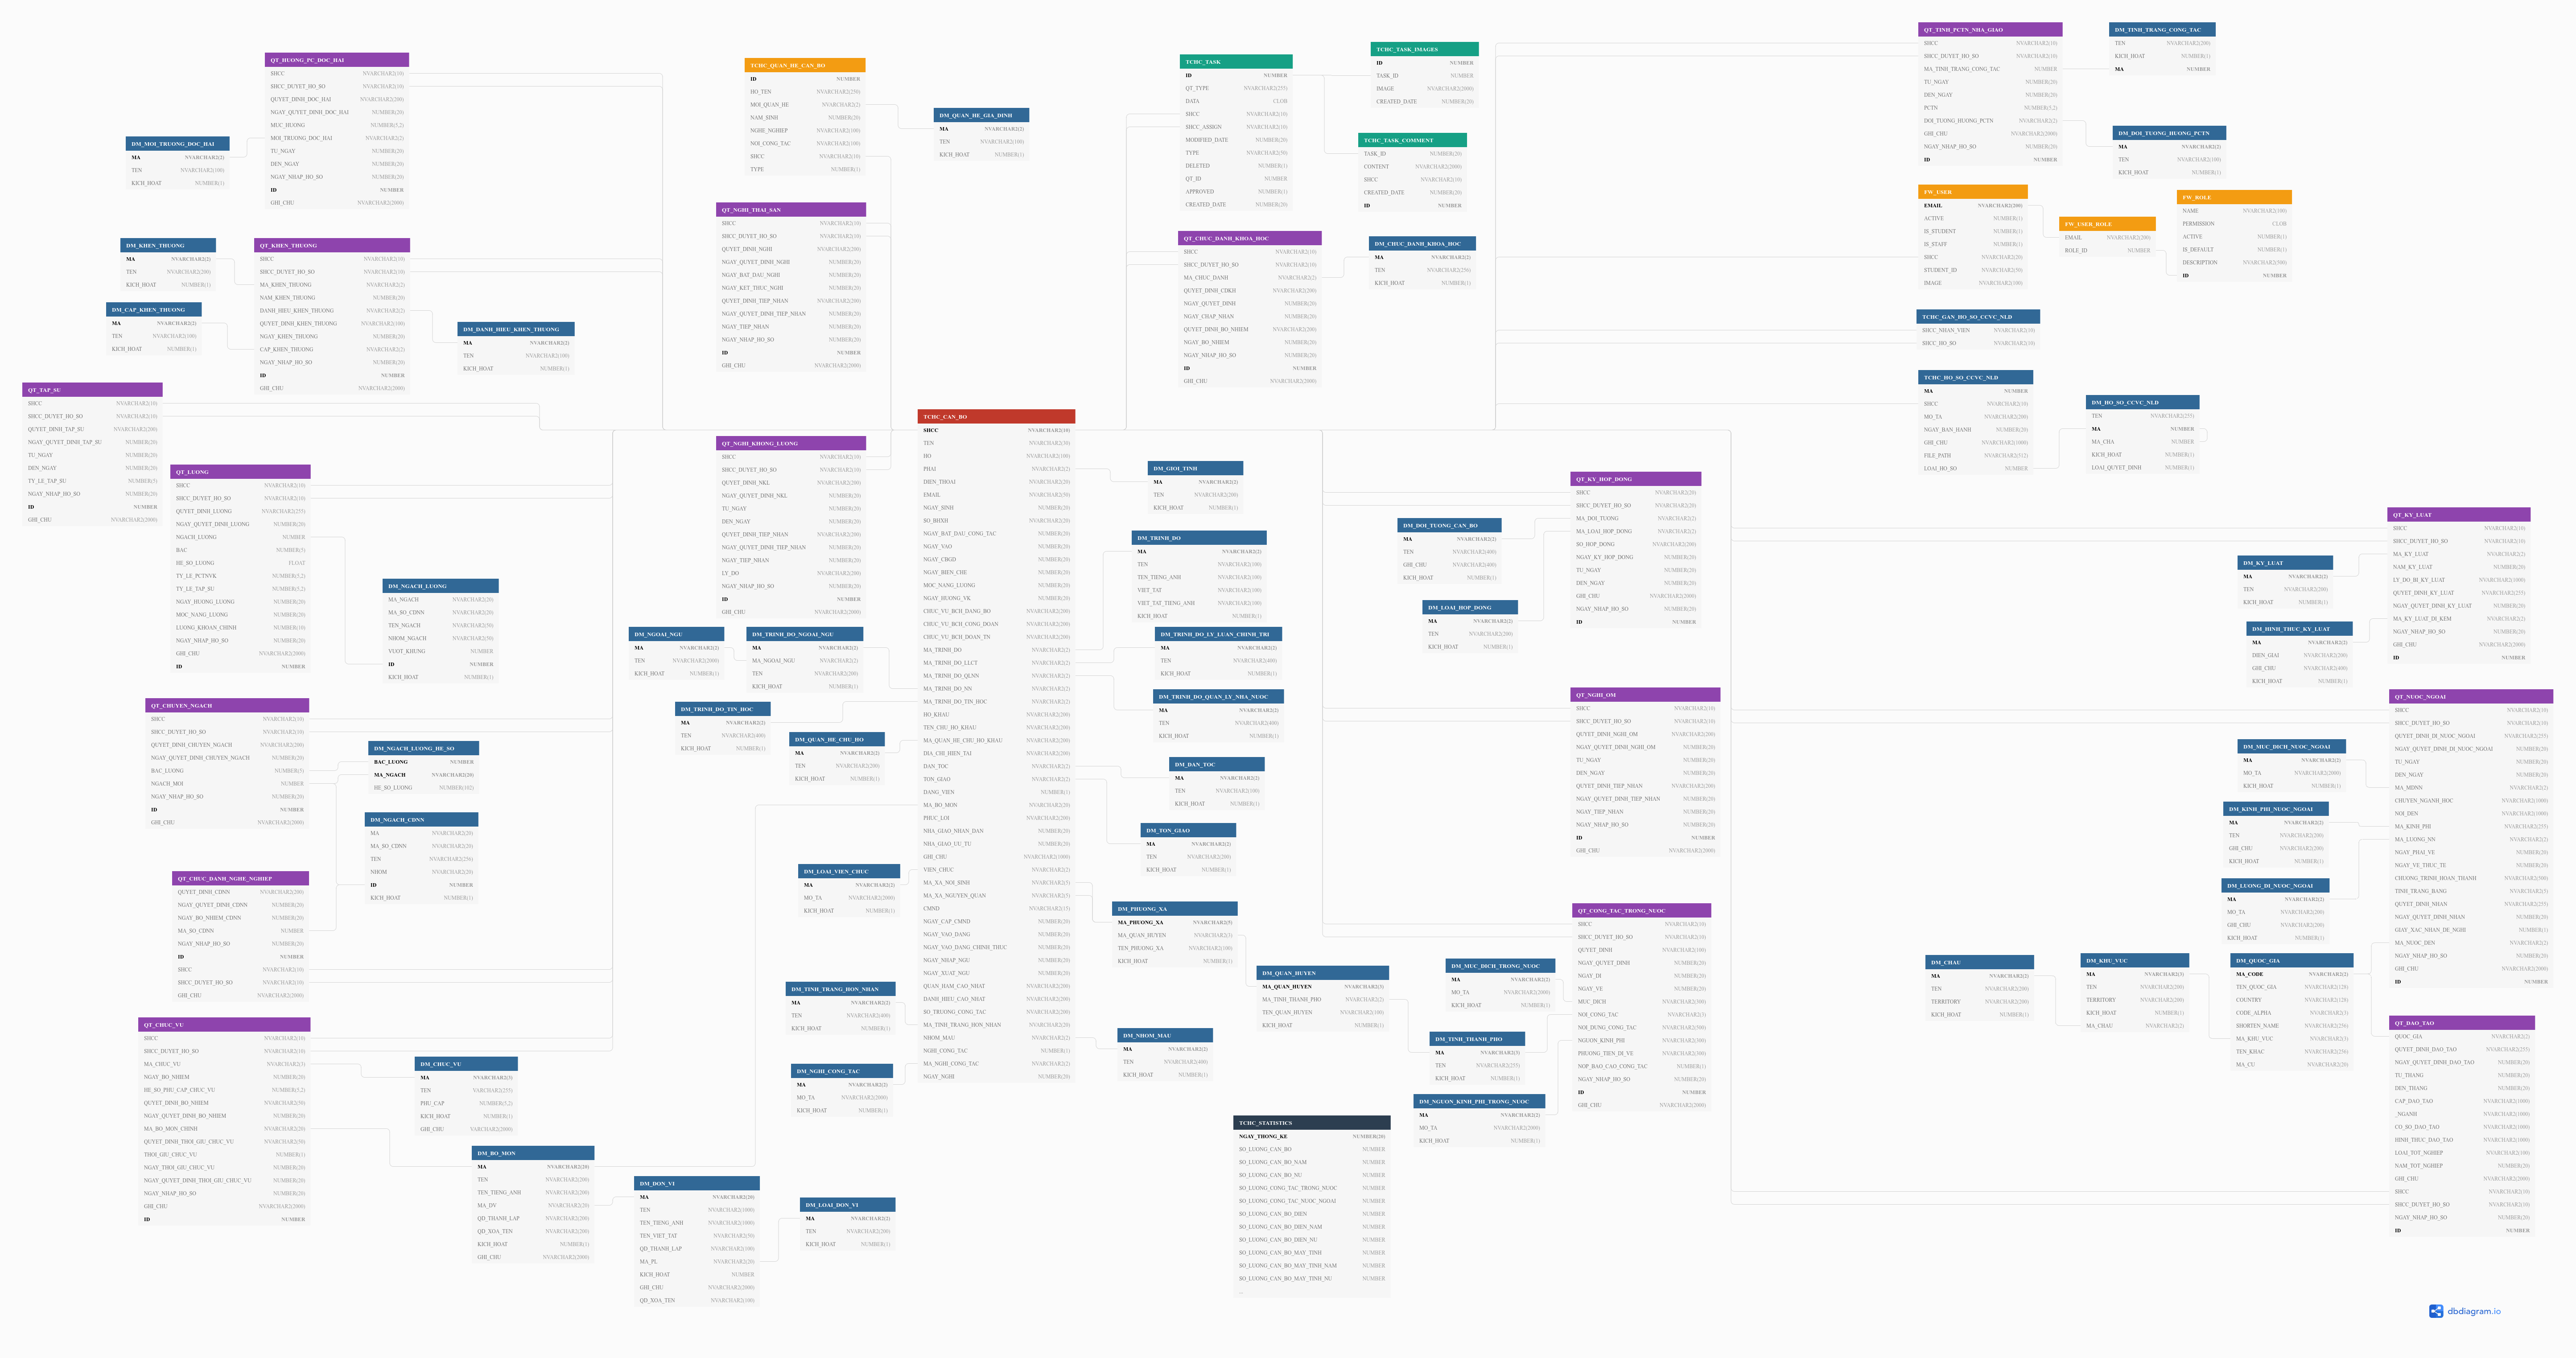
\includegraphics[width=15cm]{img/Screen/dbdiagram.png}
  \captionof{figure}{Thiết kế cơ sở dữ liệu của hệ thống}
\end{center}
Chi tiết xem ở tài liệu đính kèm.
\newpage

\chapter{\textbf{HIỆN THỰC HỆ THỐNG}}
\newpage
\section{Xác thực đối tượng người dùng}
Hệ thống xác thực đối tượng người dùng bằng hệ thống xác thực tập trung (SSO) của trường Đại học Bách Khoa - ĐHQG-HCM.
\begin{center}
  \captionsetup{type=figure}
  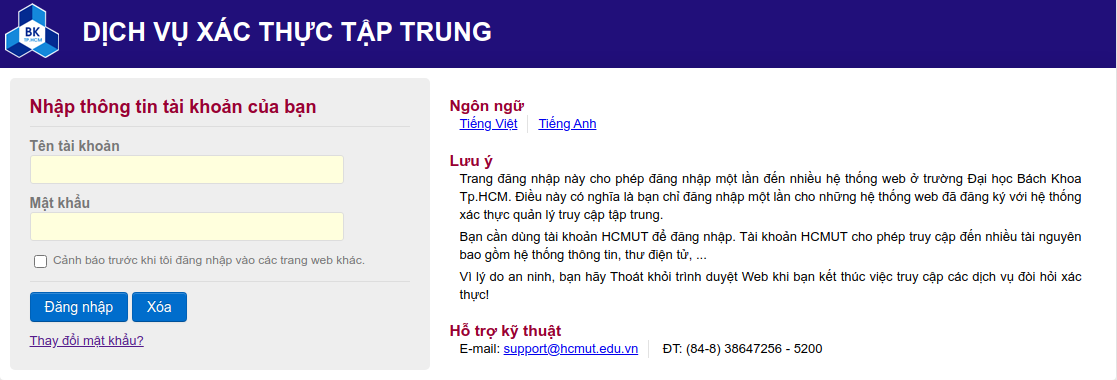
\includegraphics[width=15cm]{img/Screen/sso.png}
  \captionof{figure}{Hệ thống xác thực tập trung}
\end{center}

Người dùng sử dụng tài khoản trường Đại học Bách Khoa của mình để đăng nhập. Sau khi đăng nhập thành công, hệ thống xác thực tập trung (SSO) sẽ trả về cho hệ thống email tài khoản của người dùng. Lúc này hệ thống sẽ kiểm tra, email nhận được đã được quản trị viên thêm vào hệ thống thì người dùng sẽ đăng nhập được vào hệ thống và thực hiện các chức năng với vai trò của mình.\\

Đối với từng vai trò, sau khi đăng nhập vào hệ thống sẽ có các menu như sau:
\begin{center}
  \captionsetup{type=figure}
  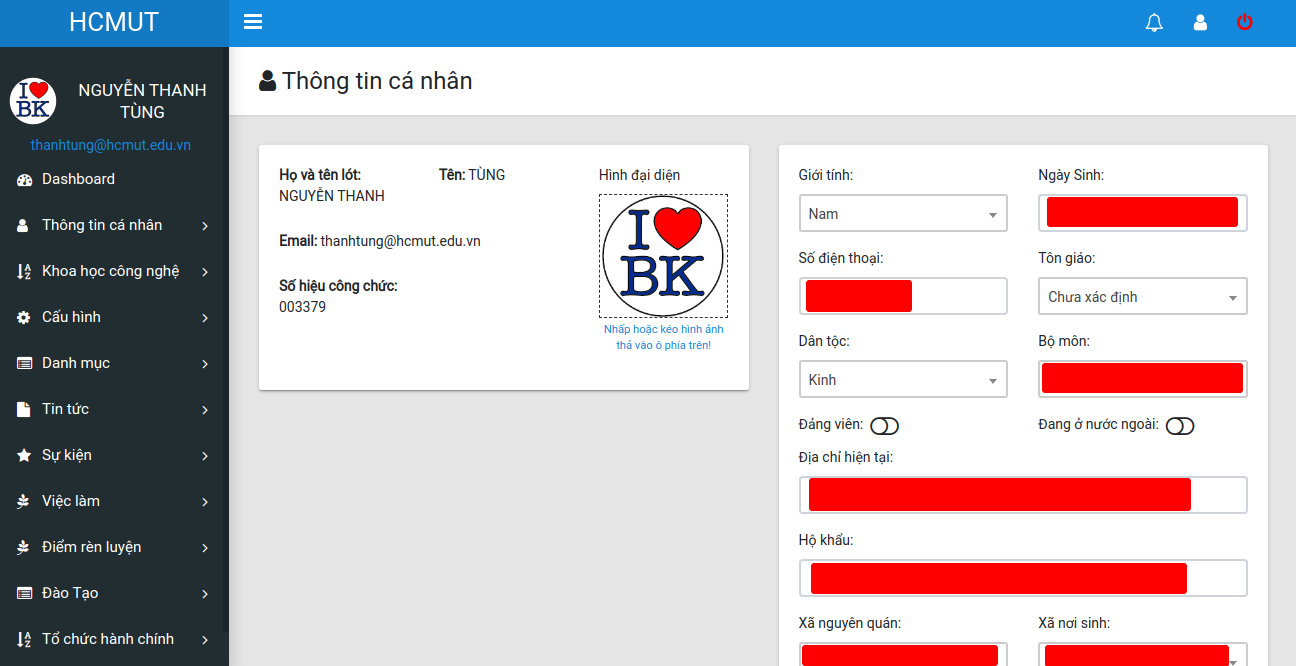
\includegraphics[width=15cm]{img/Screen/admin.png}
  \captionof{figure}{Menu của người dùng là quản trị hệ thống}
\end{center}
\begin{center}
  \captionsetup{type=figure}
  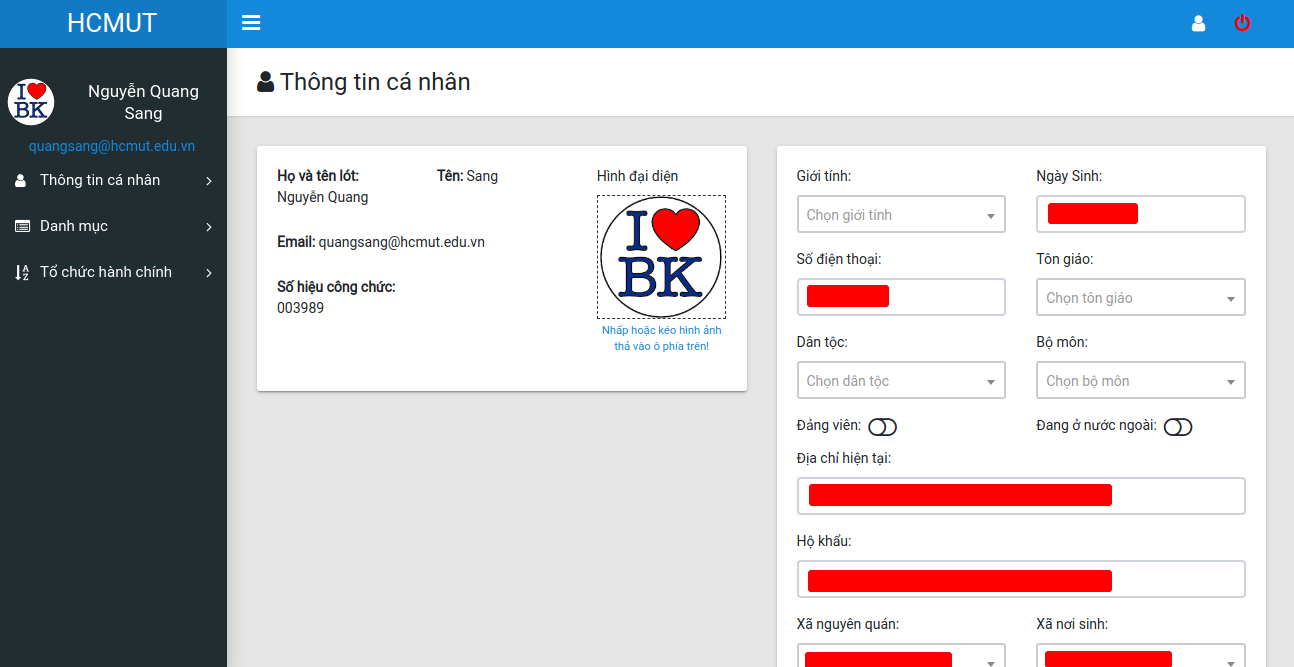
\includegraphics[width=15cm]{img/Screen/manager.png}
  \captionof{figure}{Menu của người dùng là quản lý và cán bộ phòng Tổ chức - Hành chính}
\end{center}
\begin{center}
  \captionsetup{type=figure}
  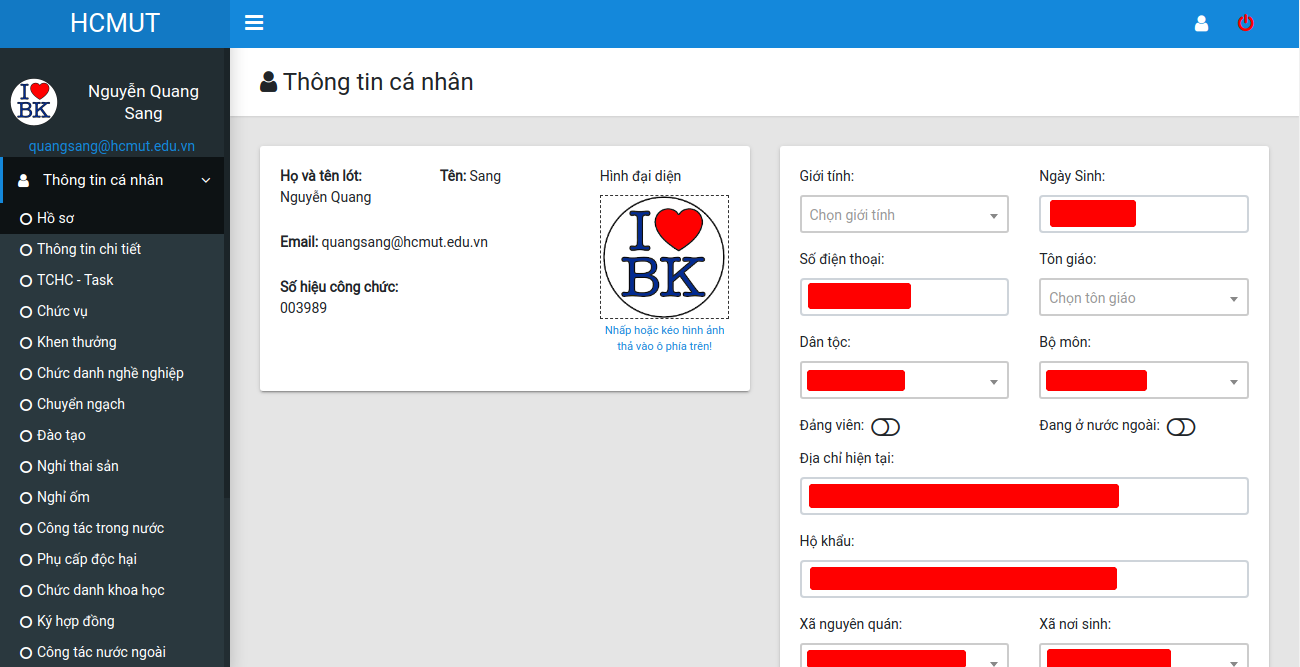
\includegraphics[width=15cm]{img/Screen/canbo.png}
  \captionof{figure}{Menu của người dùng là CBCNV của trường}
\end{center}
\section{Chức năng từng đối tượng trong hệ thống}
Từ việc thiết kế Usecase ở chương 4, nhóm nghiên cứu tiến hành thực hiện từng chức năng tương ứng với mỗi đối tượng. Cụ thể từng chức năng quan trọng như sau:
\subsection{Đối tượng: Quản trị hệ thống}
\subsubsection{Chức năng: Quản lý tài khoản người dùng}
 \begin{center}
  \captionsetup{type=figure}
  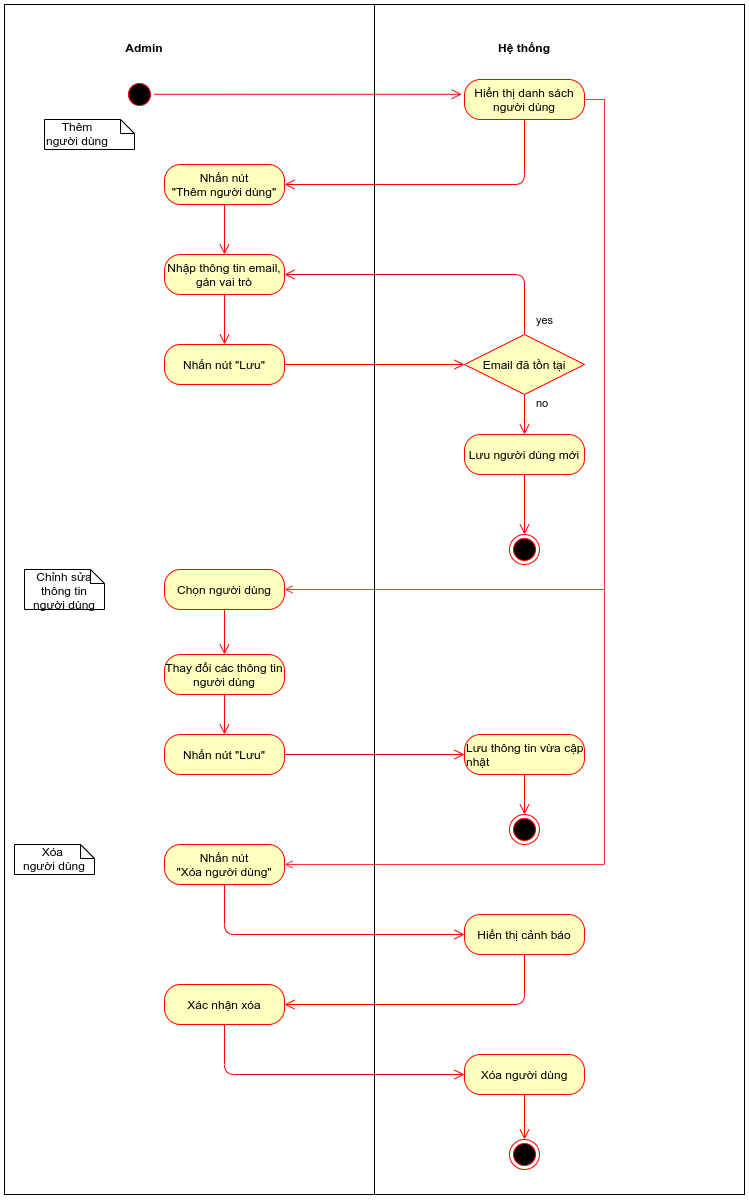
\includegraphics[width=12cm]{img/UML/Admin/UserMgt.png}
  \captionof{figure}{Lược đồ Activity quản lý tài khoản người dùng}
\end{center}
\begin{figure}[H]
    \centering
    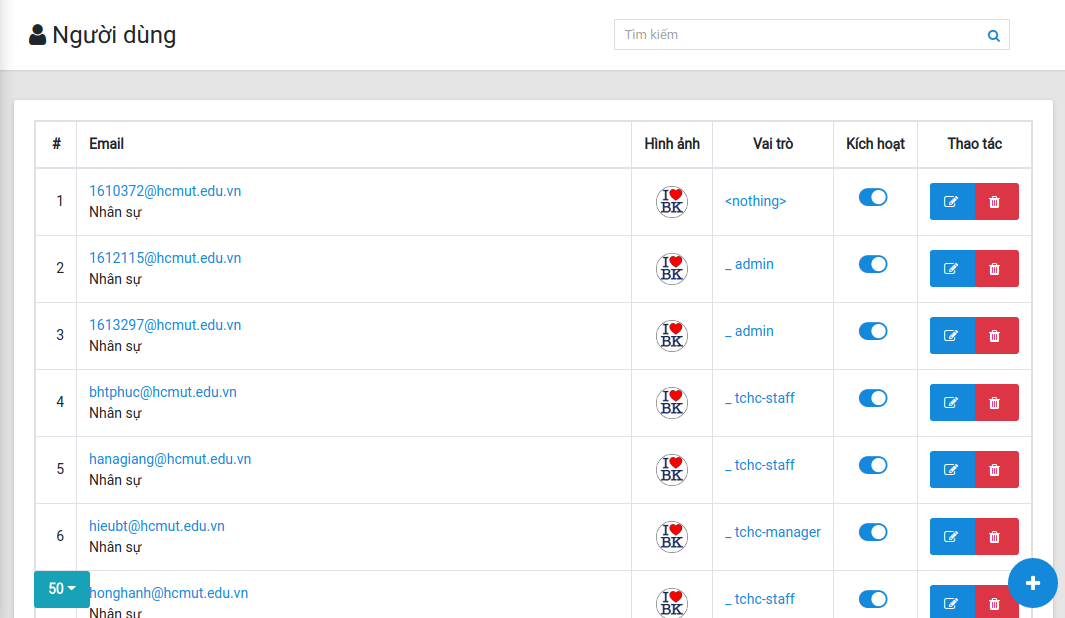
\includegraphics[width=15cm]{img/Screen/user.png}
    \caption{Danh sách người dùng hiện có của hệ thống}
    \label{fig:fig_danh_sach_nguoi_dung}
\end{figure}
Phần này giúp quản trị viên quản lý được người dùng trong hệ thống. Quản trị viên có xem danh toàn bộ người dùng (hình \ref{fig:fig_danh_sach_nguoi_dung}); chỉnh sửa các thông tin của từng người dùng, đặt vai trò trong hệ thống, kích hoạt tài khoản (hình \ref{fig:fig_edit_nguoi_dung}), xóa người dùng khỏi hệ thổng.\\
\begin{figure}[H]
    \centering
    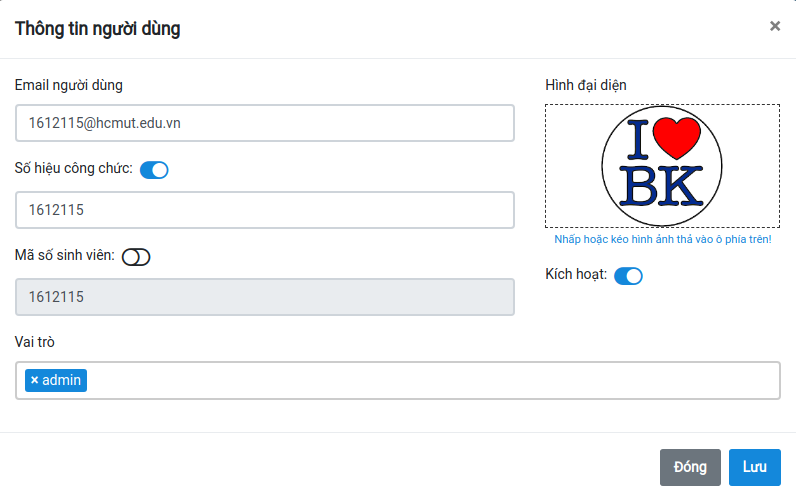
\includegraphics[width=15cm]{img/Screen/editUser.png}
    \caption{Chỉnh sửa thông tin người dùng}
    \label{fig:fig_edit_nguoi_dung}
\end{figure}
\subsubsection{Chức năng: Quản lý vai trò trong hệ thống}
\begin{center}
  \captionsetup{type=figure}
  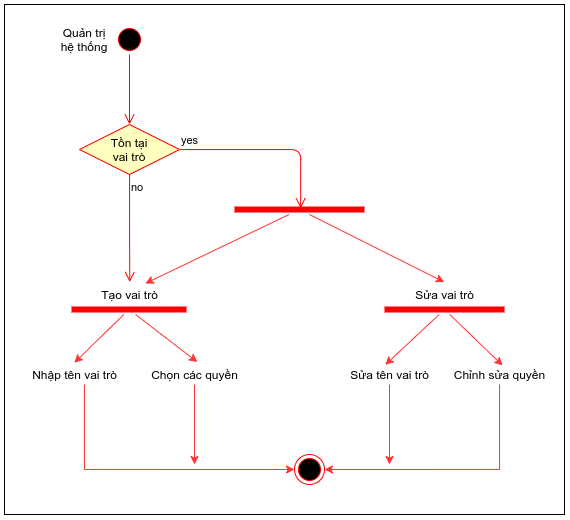
\includegraphics[width=15cm]{img/UML/Admin/addRole.png}
  \captionof{figure}{Lược đồ Activity quản lý vai trò hệ thống}
\end{center}

Hệ thống tồn tại cơ chế quản lý vai trò động. Mỗi vai trò được gán với các quyền truy cập. Quản trị viên có thể chỉnh sửa quyền của các vai trò một cách dễ dàng.\\
\begin{center}
  \captionsetup{type=figure}
  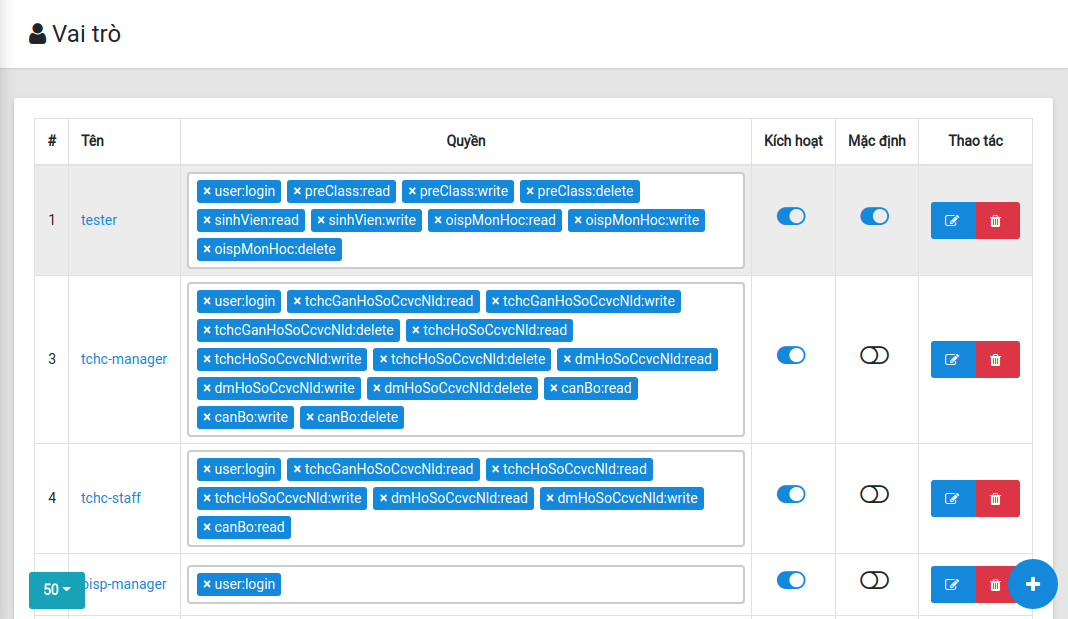
\includegraphics[width=15cm]{img/Screen/allrole.png}
  \captionof{figure}{Danh sách vai trò có trong hệ thống hiện tại}
\end{center}
\begin{center}
  \captionsetup{type=figure}
  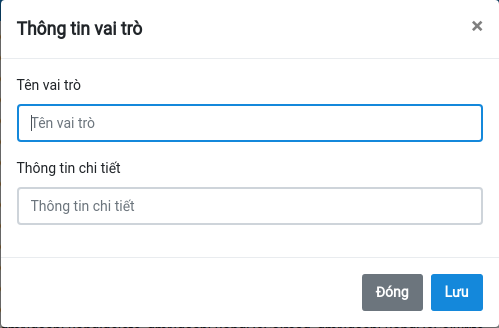
\includegraphics[width=15cm]{img/Screen/addrole.png}
  \captionof{figure}{Thêm một vai trò vào hệ thống}
\end{center}
\begin{center}
  \captionsetup{type=figure}
  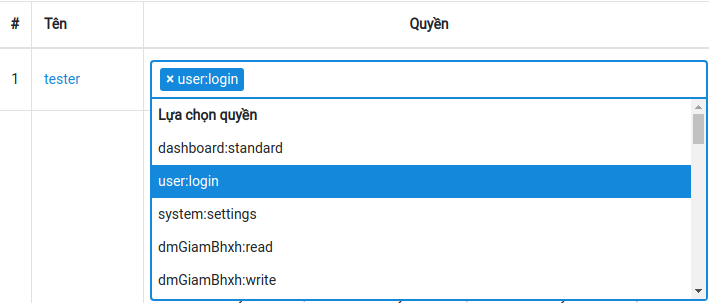
\includegraphics[width=15cm]{img/Screen/ganquyen.png}
  \captionof{figure}{Thay đổi các quyền cho vai trò}
\end{center}
\subsubsection{Chức năng: Quản lý trang chủ}
\textbf{Tạo, chỉnh sửa menu}
\begin{center}
  \captionsetup{type=figure}
  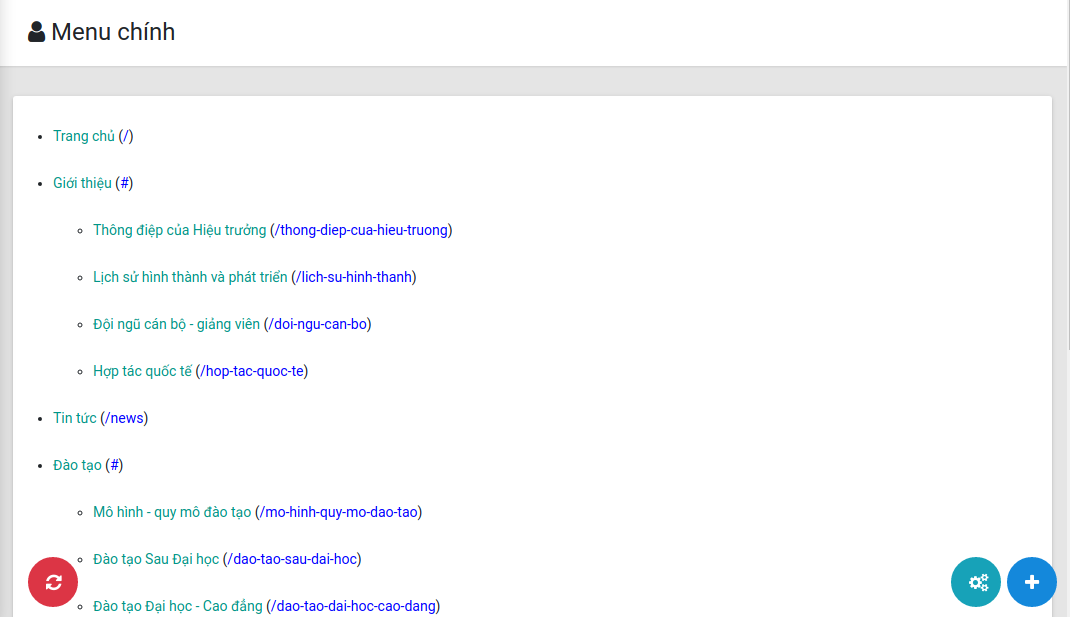
\includegraphics[width=15cm]{img/Screen/menu.png}
  \captionof{figure}{Danh sách menu của trang}
\end{center}

Phần này giúp quản trị viên thiết kế phần menu header của trang chủ như là: tạo mới menu kèm theo đường dẫn, tạo menu con, kích hoạt menu, thay đổi thứ tự hiển thị.\\

\textbf{Chức năng: Cấu hình các Section trong một trang giao diện cụ thể}
\begin{center}
  \captionsetup{type=figure}
  \includegraphics[width=15cm]{img/Screen/section.png}
  \captionof{figure}{Danh sách section của một trang giao diện cụ thể}
\end{center}

Ở một trang chủ cụ thể, quản trị viên có thể thiết lập trang đó gồm những thành phần nào và thứ tự xuất hiện của các thành phần đó.\\

\textbf{Chức năng: Quản lý thông tin danh mục}\\
\begin{center}
  \captionsetup{type=figure}
  \includegraphics[width=15cm]{img/UML/Admin/danhmucActivity.png}
  \captionof{figure}{Lược đồ Activity quản lý danh mục}
\end{center}

Chức năng cho phép người quản trị hệ thống quy định các thông tin danh mục phục vụ cho việc nhập và lưu dữ liệu.\\
\begin{center}
  \captionsetup{type=figure}
  \includegraphics[width=15cm]{img/Screen/danhmuc.png}
  \captionof{figure}{Danh sách danh mục bộ môn}
\end{center}
\subsection{Đối tượng: Quản lý phòng Tổ chức - Hành chính}
\subsubsection{Chức năng: Quản lý nhân viên phòng Tổ chức - Hành chính}
\begin{center}
  \captionsetup{type=figure}
  \includegraphics[width=15cm]{img/UML/Manager/assignTask.png}
  \captionof{figure}{Lược đồ Activity cho chức năng phân công cán bộ duyệt yêu cầu}
\end{center}
\begin{figure}[H]
    \centering
    \begin{subfigure}[b]{0.4\linewidth}
        \includegraphics[width=\linewidth]{img/Screen/assignhoso.png}
        \caption{Phân công cán bộ nhập hồ sơ}
        \label{fig:assign_hoso}
    \end{subfigure}
    \begin{subfigure}[b]{0.4\linewidth}
        \includegraphics[width=\linewidth]{img/Screen/assignTask.png}
        \caption{Phân công cán bộ duyệt yêu cầu}
        \label{fig:assign_task}
    \end{subfigure}
    \caption{Phân công cho cán bộ phòng Tổ chức - Hành chính}
\end{figure}
\subsubsection{Chức năng cấu hình phòng Tổ chức - Hành chính}
\textbf{Cấu hình thông tin email cho phòng Tổ chức - Hành chính}
\begin{figure}[H]
    \centering
    \begin{subfigure}[b]{0.4\linewidth}
        \includegraphics[width=\linewidth]{img/Screen/emailsetting.png}
        \caption{Cấu hình địa chỉ email}
        \label{fig:email_setting}
    \end{subfigure}
    \begin{subfigure}[b]{0.4\linewidth}
        \includegraphics[width=\linewidth]{img/Screen/email.png}
        \caption{Cấu hình nội dung các email}
        \label{fig:email}
    \end{subfigure}
    \caption{Cấu hình email cho phòng Tổ chức - Hành chính}
\end{figure}

Phần này giúp quản trị viên thực hiện việc \textbf{soạn thảo nội dung} của email và nội dung của email này sẽ được sử dụng để thông báo cho những người dùng liên quan khi có các hoạt động liên quan đến yêu cầu. Trong nội dung của email, hệ thống có cung cấp những \textbf{tham số} được sử dụng khi cần thiết. Các tham số này sẽ được thay thế bằng những từ phù hợp bởi hệ thống trước khi gửi đi cho người dùng.\\

Ngoài ra, người quản lý phòng Tổ chức - Hành chính còn quản lý các danh mục liên quan đến phòng Tổ chức - Hành chính.
\subsubsection{Chức năng: Xem những thống kê của hệ thống}
\begin{center}
  \captionsetup{type=figure}
  \includegraphics[width=15cm]{img/UML/User/dashboard.png}
  \captionof{figure}{Xem thống kê}
\end{center}

Quản lý phòng Tổ chức - Hành chính có thể theo dõi những thống kê trong hệ thống dưới dạng biểu đồ trực quan, sinh động. Thống kê về một số dữ liệu như:
\begin{itemize}
    \item Số nhân viên phòng Tổ chức - Hành chính
    \item Số lượng hồ sơ được nhận trong tháng
    \item Tỉ lệ yêu cầu phân chia theo loại
    \item Tỉ lệ yêu cầu phân chia theo trạng thái
    \item Tỉ lệ giới tính của cán bộ
    \item Tỉ lệ giới tính của cán bộ theo 13 khoa
    \item Số lượng cán bộ đang công tác trong nước
    \item Số lượng cán bộ đang công tác nước ngoài
    \item Số lượng, tỉ lệ sinh viên theo các khoá
\end{itemize}
\subsection{Đối tượng: Cán bộ phòng Tổ chức - Hành chính}
\subsubsection{Chức năng: Gán hồ sơ công chức, viên chức cho cán bộ}
\begin{center}
  \captionsetup{type=figure}
  \includegraphics[width=15cm]{img/UML/TchcStaff/activityQuanLyHoSo.png}
  \captionof{figure}{Lược đồ Activity quản lý hồ sơ cán bộ}
\end{center}

Chức năng cho phép quản lý các hồ sơ của cán bộ. Lưu trữ hồ sơ gốc dưới dạng tệp trên hệ thống.
\begin{center}
  \captionsetup{type=figure}
  \includegraphics[width=15cm]{img/Screen/qlhoso.png}
  \captionof{figure}{Quản lý hồ sơ cán của một cán bộ}
\end{center}
\textbf{Chức năng: Quản lý cán bộ}\\
\begin{center}
  \captionsetup{type=figure}
  \includegraphics[width=15cm]{img/UML/TchcStaff/activityQuanLyCanBo.png}
  \captionof{figure}{Lược đồ Activity chức năng quản lý thông tin cán bộ}
\end{center}

Đây là chức năng cho phép đối tượng là cán bộ phòng Tổ chức - Hành chính có thể xem và chỉnh sửa thông tin của toàn bộ cán bộ hiện có trong hệ thống, thêm cán bộ vào hệ thống, xóa cán bộ khỏi hệ thống. Bên cạnh đó họ còn có thể xuất thông tin của cán bộ ra tệp tin Word theo mẫu của Bộ nội vụ.\\
\begin{center}
  \captionsetup{type=figure}
  \includegraphics[width=15cm]{img/Screen/allcanbo.png}
  \captionof{figure}{Danh sách toàn bộ cán bộ}
\end{center}
\begin{center}
  \captionsetup{type=figure}
  \includegraphics[width=15cm]{img/Screen/editthongtin.png}
  \captionof{figure}{Xem, chỉnh sửa thông tin cán bộ}
\end{center}
\subsubsection{Chức năng: Quản lý đối với một quá trình nghiệp vụ}
\begin{center}
  \captionsetup{type=figure}
  \includegraphics[width=15cm]{img/UML/TchcStaff/activityQuanLyQT.png}
  \captionof{figure}{Lược đồ Activity quản lý quá trình nghiệp vụ}
\end{center}

Chức năng này cho phép cán bộ phòng Tổ chức - Hành chính quản lý các quá trình nghiệp vụ của cán bộ trong trường. Cán bộ có thể thêm mới, chỉnh sửa hoặc xóa thông tin một quá trình. Ngoài ra, có thể tải toàn thông tin của quá trình dưới dạng tệp Excel.\\
\begin{center}
  \captionsetup{type=figure}
  \includegraphics[width=15cm]{img/Screen/qlquatrinh.png}
  \captionof{figure}{Quản lý quá trình chức vụ của cán bộ}
\end{center}
\subsubsection{Chức năng: Quản lý các yêu cầu của cán bộ}
\begin{center}
  \captionsetup{type=figure}
  \includegraphics[width=15cm]{img/UML/TchcStaff/activityQLTask.png}
  \captionof{figure}{Lược đồ Activity cho chức năng quản lý các yêu cầu của người dùng}
\end{center}
\begin{center}
  \captionsetup{type=figure}
  \includegraphics[width=15cm]{img/Screen/qltask.png}
  \captionof{figure}{Xem toàn bộ yêu cầu của cán bộ}
\end{center}

\begin{center}
  \captionsetup{type=figure}
  \includegraphics[width=15cm]{img/Screen/chitiettask.png}
  \captionof{figure}{Xem thông tin chi tiết yêu cầu của cán bộ}
\end{center}
Khi xem chi tiết yêu cầu, cán bộ phòng Tổ chức - Hành chính có thể chỉnh sửa thông tin mà người dùng yêu cầu, sau đó đồng ý hoặc từ chứ duyệt yêu cầu. Bên cạnh đó cán bộ có thể để lại bình luận kèm theo những hình ảnh mình chứng (nếu có) cho yêu cầu.\\
\subsection{Đối tượng: Cán bộ, công nhân viên của nhà trường}
\subsubsection{Chức năng: Quản lý thông tin}
\begin{center}
  \captionsetup{type=figure}
  \includegraphics[width=15cm]{img/UML/User/activityQLThongTin.png}
  \captionof{figure}{Lược đồ Activity cho chức năng quản lý thông tin cho cán bộ}
\end{center}
\subsubsection{Chức năng: Quản lý quá trình}
\begin{center}
  \captionsetup{type=figure}
  \includegraphics[width=15cm]{img/UML/User/activityQuanLyQT.png}
  \captionof{figure}{Lược đồ Activity cho chức năng quản lý quá trình cho cán bộ}
\end{center}

\subsubsection{Chức năng: Quản lý yêu cầu}
\begin{center}
  \captionsetup{type=figure}
  \includegraphics[width=15cm]{img/UML/User/activityQLTask.png}
  \captionof{figure}{Lược đồ Activity cho chức năng quản lý yêu cầu của cán bộ}
\end{center}
\newpage

\chapter{\textbf{KIỂM THỬ}}
\newpage
Kiểm thử phần mềm là một bước quan trọng trong quy trình phát triển phần mềm, đảm bảo sản phẩm đáp ứng đầy đủ, chính xác những yêu cầu của khách hàng, giúp nhà phát triển phát hiện ra các lỗi tiềm ẩn, giảm thiểu các rủi ro và chi phí phát sinh trong quá trình bảo dưỡng và nâng cấp phần mềm trong tương lai.

Hệ thống website phòng Tổ chức-Hành chính được sử dụng trong việc quản lý thông tin, nghiệp vụ của cán bộ nhân viên nhà trường, vì vậy hệ thống phải đảm bảo được tính bảo mật, chính xác trong các tác vụ, tránh các lỗi gây ảnh hưởng, gián đoạn công việc của phòng Tổ chức-Hành chính và cán bộ nhân viên nhà trường. Vì vậy việc kiểm thử là vô cùng quan trọng và cần thiết trong quá trình xây dựng hệ thống.

Các công nghệ sử dụng trong kiểm thử thử hệ thống:
\begin{center}
  \captionsetup{type=figure}
  \includegraphics[width=10cm]{img/mocha_chai.png}
  \captionof{figure}{Mocha framework và Chai assertion library}
\end{center}

Mocha là một Javascript framework kiểm thử chạy trên Node.js và trình duyệt, giúp cho việc kiểm tra bất đồng bộ một cách đơn giản. Mocha được đánh giá là một framework kiểm thử đơn giản, linh hoạt và chạy ổn định. Hiện nay, Mocha được nhiều công ty lớn sử dụng trong kiểm thử hệ thống.

Chai là một thư viện assertion với nhiều tuỳ chọn cho phép kiểm tra đối tượng như "should", "expect" và "assert". Trong hệ thống Tổ chức-Hành chính, nhóm nhận thấy có nhiều API có phương thức GET trả về dữ liệu dưới dạng JSON nên nhóm sử dụng Chai để thực hiện HTTP request và kiểm tra các giá trị trả về.

Nhận thấy sự đơn giản và phù hợp của Mocha framework và Chai assertion library, nhóm đã xây dựng hệ thống kiểm thử với 2 công nghệ trên để đảm bảo hệ thống hoạt động một cách tốt nhất khi đưa vào thực tế.

\section{Kiểm thử đơn vị (Unit Test)}
Kiểm thử đơn vị là một loại kiểm thử phần mềm, trong đó các thành phần đơn vị như method, class, function sẽ được kiểm thử. Kiểm thử đơn vị nhằm kiểm tra các tính năng riêng lẻ hoạt động đúng hay không. Ở phần này, nhóm kiểm thử các hàm xử lý thời gian, chuỗi, kiểm tra email,...
\begin{center}
  \captionsetup{type=figure}
  \includegraphics[width=15cm]{img/unitTestCode.png}
  \captionof{figure}{Đoạn code kiểm thử các hàm xử lý thời gian, chuỗi, kiểm tra email}
\end{center}
\newpage
Kết quả: 

\begin{center}
  \captionsetup{type=figure}
  \includegraphics[width=7cm]{img/unitTestSolution.png}
  \captionof{figure}{Kết quả kiểm thử đơn vị}
\end{center}
\section{Kiểm thử tích hợp (Integration Test)}
Kiểm thử tích hợp là một giai đoạn trong kiểm thử phần mềm xảy ra sau khi kiểm thử đơn vị. Mục đích của kiểm thử tích hợp nhằm kiểm tra sự giao tiếp giữa các module, nhằm đảm bảo tính hợp nhất của hệ thống.
Nhóm đã sử dụng Mocha framework và Chai library để kiểm thử các API giao tiếp giữa tầng View và Controller.
\begin{center}
  \captionsetup{type=figure}
  \includegraphics[width=15cm]{img/integrationTestCode.png}
  \captionof{figure}{Đoạn code kiểm thử các API giao tiếp giữa tầng View và Controller}
\end{center}
\newpage
Kết quả:
\begin{center}
  \captionsetup{type=figure}
  \includegraphics[width=15cm]{img/integrationTestSolution.png}
  \captionof{figure}{Kết quả kiểm thử tích hợp}
\end{center}
\section{Kiểm thử hệ thống (System Test)}
Kiểm thử hệ thống là giai đoạn kiểm thử nhằm kiểm tra sự hoàn chỉnh và tích hợp đầy đủ của hệ thống. Kiểm thử hệ thống là phương pháp kiểm thử hộp đen vì chỉ kiểm thử thông qua giao diện bên ngoài. Phương pháp kiểm thử này nhằm mục đích tìm ra các lỗi như:
\begin{itemize}
    \item Chức năng thiếu hoặc không chính xác.
    \item Lỗi truy cập cơ sở dữ liệu từ bên ngoài.
    \item Lỗi giao diện.
    \item Lỗi hiệu suất.
\end{itemize}
Trong quá trình phát triển hệ thống, nhóm tiến hành kiểm thử các chức năng của hệ thống như xem, tạo mới, sửa đổi, xoá thông tin với nhiều vai trò khác nhau như cán bộ phòng Tổ chức-Hành chính và người dùng hệ thống.
\subsection{Quy trình kiểm thử quản lý quá trình công tác trong nước với vai trò cán bộ phòng Tổ chức-Hành chính}
Tạo mới quá trình -> Chỉnh sửa quá trình -> Xoá quá trình

Danh sách quá trình công tác trong nước ban đầu.
\begin{center}
  \captionsetup{type=figure}
  \includegraphics[width=15cm]{img/test/viewFirst.png}
  \captionof{figure}{Danh sách quá trình công tác trong nước ban đầu}
\end{center}
Tạo mới một quá trình
\begin{center}
  \captionsetup{type=figure}
  \includegraphics[width=10cm]{img/test/newForm.png}
  \captionof{figure}{Tạo mới quá tình công tác trong nước}
\end{center}
Tạo mới quá trình công tác trong nước thành công
\begin{center}
  \captionsetup{type=figure}
  \includegraphics[width=10cm]{img/test/aleartNew.png}
  \captionof{figure}{Tạo mới quá tình công tác trong nước thành công}
\end{center}
\newpage
Quá trình mới tạo được thêm vào danh sách
\begin{center}
  \captionsetup{type=figure}
  \includegraphics[width=15cm]{img/test/viewNew.png}
  \captionof{figure}{Danh sách quá trình trong nước sau khi tạo mới thành công}
\end{center}
Chỉnh sửa quá trình:
\begin{center}
  \captionsetup{type=figure}
  \includegraphics[width=15cm]{img/test/editForm.png}
  \captionof{figure}{Chỉnh sửa quá tình công tác trong nước}
\end{center}
Chỉnh sửa thành công:
\begin{center}
  \captionsetup{type=figure}
  \includegraphics[width=10cm]{img/test/aleartEdit.png}
  \captionof{figure}{Chỉnh sửa quá tình công tác trong nước thành công}
\end{center}
Quá trình công tác trong nước đã được thay đổi.
\begin{center}
  \captionsetup{type=figure}
  \includegraphics[width=15cm]{img/test/viewEdit.png}
  \captionof{figure}{Danh sách quá trình trong nước sau khi chỉnh sửa thành công}
\end{center}
Xoá quá trình:
\begin{center}
  \captionsetup{type=figure}
  \includegraphics[width=10cm]{img/test/confirmDelete.png}
  \captionof{figure}{xác nhận xoá quá trình công tác trong nước}
\end{center}
Xoá thành công:
\begin{center}
  \captionsetup{type=figure}
  \includegraphics[width=10cm]{img/test/aleartDelete.png}
  \captionof{figure}{Xoá quá tình công tác trong nước thành công}
\end{center}
Danh sách quá trình công tác trong nước sau khi xoá thành công
\begin{center}
  \captionsetup{type=figure}
  \includegraphics[width=15cm]{img/test/viewFirst.png}
  \captionof{figure}{Danh sách quá trình công tác trong nước sau khi xoá thành công}
\end{center}
\subsection{Quy trình kiểm thử tạo yêu cầu thêm, sửa, xoá quá trình với vai trò người dùng hệ thống}
Danh sách quá trình công tác trong nước của người dùng được hiển thị.
\begin{center}
  \captionsetup{type=figure}
  \includegraphics[width=15cm]{img/test/userView.png}
  \captionof{figure}{Danh sách quá trình công tác trong nước của người dùng}
\end{center}
Tạo yêu cầu tạo mới quá trình.
\begin{center}
  \captionsetup{type=figure}
  \includegraphics[width=15cm]{img/test/userForm.png}
  \captionof{figure}{Tạo yêu cầu tạo mới quá trình công tác trong nước}
\end{center}
Yêu cầu được thêm vào danh sách yêu cầu
\begin{center}
  \captionsetup{type=figure}
  \includegraphics[width=15cm]{img/test/userTask.png}
  \captionof{figure}{Danh sách các yêu cầu của cá nhân người dùng}
\end{center}
Xem chi tiết và chỉnh sửa lại yêu cầu
\begin{center}
  \captionsetup{type=figure}
  \includegraphics[width=15cm]{img/test/taskDetailUser.png}
  \captionof{figure}{Chi tiết yêu cầu của người dùng}
\end{center}
\subsection{Quy trình kiểm thử duyệt yêu cầu với vai trò cán bộ phòng Tổ chức-Hành chính}
Xem danh sách các yêu cầu
\begin{center}
  \captionsetup{type=figure}
  \includegraphics[width=15cm]{img/test/adminTask.png}
  \captionof{figure}{Danh sách các yêu cầu của tất cả người dùng}
\end{center}

\newpage Trưởng phòng giao yêu cầu cho cán bộ để xem xét
\begin{center}
  \captionsetup{type=figure}
  \includegraphics[width=15cm]{img/test/assignAdmin.png}
  \captionof{figure}{Giao yêu cầu cho cán bộ phòng Tổ chức - Hành chính xử lý}
\end{center}
Xem thông tin chi tiết yêu cầu
\begin{center}
  \captionsetup{type=figure}
  \includegraphics[width=15cm]{img/test/taskDetailAdmin.png}
  \captionof{figure}{Chi tiết yêu cầu}
\end{center}

Duyệt yêu cầu
\begin{center}
  \captionsetup{type=figure}
  \includegraphics[width=10cm]{img/test/confirmApprove.png}
  \captionof{figure}{Xác nhận duyệt yêu cầu}
\end{center}
Yêu cầu đã được duyệt thành công
\begin{center}
  \captionsetup{type=figure}
  \includegraphics[width=15cm]{img/test/approved.png}
  \captionof{figure}{Duyệt yêu cầu thành công}
\end{center}
Một quá trình công tác trong nước mới đã được thêm vào danh sách quá trình công tác trong nước.
\begin{center}
  \captionsetup{type=figure}
  \includegraphics[width=15cm]{img/test/viewLast.png}
  \captionof{figure}{Một quá trình mới được thêm vào danh sách quá trình công tác trong nước}
\end{center}
\section{Kiểm thử chấp nhận (Acceptance Test)}
Kiểm thử chấp nhận là quá trình kiểm thử được thực hiện bởi khách hàng để xác nhận hệ thống có hoạt động đúng như mong đợi với các yêu cầu của khách hàng. Đây là giai đoạn thử nghiệm cuối cùng trước khi hệ thống được đưa vào hoạt động chính thức. 

Hệ thống sẽ được bàn giao với cán bộ phòng Tổ chức-Hành chính để kiểm tra lần cuối trước khi đưa vào sử dụng.
\newpage

\chapter{\textbf{KẾT LUẬN VÀ HƯỚNG PHÁT TRIỂN}}
\newpage
\section{Kết quả đạt được}
Thông qua quá trình phân tích yêu cầu hệ thống, nghiên cứu các công nghệ và tiến hành làm luận văn, nhóm đã xây dựng thành công hệ thống phòng Tổ chức-Hành chính trên nền tảng Web. Hệ thống đã đáp ứng được các yêu cầu, nghiệp vụ được giao với giao diện hiện đại và dễ sử dụng với các tính năng nổi bật sau:
\begin{itemize}
    \item Trang chủ tổng hợp hình ảnh giới thiệu, sự kiện, tin tức và các thông tin liên hệ với giao diện phù hợp cho nhiều loại thiết bị và quản trị viên có thể tuỳ chỉnh các thành phần hiển thi.
    \item Xây dựng được chức năng quản lý CBCNV của trường bao gồm các chức năng cơ bản như sau:
        \subitem - Thêm cán bộ mới vào hệ thống.
        \subitem - Quản lý thông tin viên chức của cán bộ.
        \subitem - Quản lý các loại hồ sơ, văn bằng của cán bộ.
        \subitem - Xuất thông tin của cán bộ dưới theo mẫu của Bộ nội vụ dưới dạng tệp tin word.
    \item Xây dựng được các chức năng hỗ trợ quản lý các quá trình nghiệp vụ:
        \subitem - Đối với cán bộ của phòng Tổ chức - Hành chính có các chức năng như thêm, chỉnh sửa, xóa các quá trình nghiệp vụ của CBCNV.
        \subitem - Đối với CBCNV có thể xem được các quá trình nghiệp vụ của chính mình.
    \item Xây dựng các chức năng quản lý yêu cầu về quá trình nghiệp vụ của CBCNV:
        \subitem - Chức năng duyệt các yêu cầu đối với cán bộ phòng Tổ chức - Hành chính.
        \subitem - Chức năng tạo các yêu cầu mới cho các quá trình nghiệp vụ đối với CBCNV.
        \subitem - Thêm bình luận, hình ảnh minh chứng cho các yêu cầu
    \item Gửi email thông báo: Những người dùng liên quan sẽ nhận được mail thông báo trong các trường hợp sau:
        \subitem - Có yêu cầu mới được tạo.
        \subitem - Yêu cầu đã được chỉnh sửa.
        \subitem - Yêu cầu đã được duyệt/từ chối.
        \subitem - Yêu cầu có bình luận mới.
    \item Trang thống kê các số liệu của hệ thống.
    \item Hệ thống hỗ trợ tìm kiếm các bảng, trong mỗi bảng có hỗ trợ tìm kiếm theo các cột.
\end{itemize}
\section{Ưu điểm}
Với các chức năng đã thực hiện được, hệ thống Tổ chức - Hành chính có các ưu điểm sau:
\begin{itemize}
    \item Hệ thống đã được đưa lên máy chủ, một số chức năng đã được phòng Tổ chức - Hành chính sử dụng.
    \item Hệ thống hỗ trợ nhập liệu một cách nhanh chóng và dễ dàng.
    \item Giao diện đẹp, thân thiện với người dùng.
    \item Đơn giản hoá các quy trình nghiệp vụ rườm rà.
    \item Sử dụng được trên nhiều thiết bị.
    \item Tính bảo mật cao, phân chia chức năng theo vai trò của người dùng.
    \item Mã nguồn dưới dạng module dễ bảo trì và  phát triển thêm nghiệp vụ mới.
\end{itemize}
\section{Hạn chế}
Bên cạnh những ưu điểm nêu trên thì hệ thống còn tồn tại một vài điểm hạn chế:
\begin{itemize}
    \item Với khối lượng dữ liệu lớn, hệ thống chưa tối ưu được tốc độ xử lý.
    \item Quá trình kiểm thử được thực hiện nghiêm túc nhưng với sự phúc tạp của hệ thống không thể tránh khỏi những lỗi không mong muốn.
\end{itemize}
\section{Hướng phát triển}
Những định hướng cho hệ thống trong tương lai:
\begin{itemize}
    \item Tích hợp các cơ chế kỹ thuật khắc phục hệ thống, tự động sao lưu.
    \item Hiện thực ứng dụng trên nền tảng Mobile.
    \item Nhân rộng hệ thống cho phòng Tổ chức - Hành chính của các đơn vị, trường học khác.
\end{itemize}
\newpage
\begin{thebibliography}{80}

\bibitem{}
\url{https://nodejs.org/en/docs/}, ngày truy cập: 18/12/2019

\bibitem{}
\url{https://docs.oracle.com/en/java/}, ngày truy cập: 18/12/2019

\bibitem{}
\url{https://docs.python.org/3/}, ngày truy cập: 18/12/2019

\bibitem{}
\url{https://docs.djangoproject.com/en/3.0/}, ngày truy cập: 18/12/2019

\bibitem{}
\url{https://hoclaptrinh.vn/posts/django-la-gi}, ngày truy cập: 18/12/2019

\bibitem{}
\url{https://techmaster.vn/posts/35345/cac-framework-trong-python-nam-2019}, ngày truy cập: 18/12/2019

\bibitem{}
\url{http://flask.palletsprojects.com/en/1.1.x/}, ngày truy cập 18/12/2019


\bibitem{}
\url{https://sass-lang.com/}, ngày truy cập: 19/12/2019

\bibitem{}
\url{http://lesscss.org/}, ngày truy cập: 19/12/2019

\bibitem{}
\url{https://docs.mongodb.com/}, ngày truy cập: 20/12/2019

\bibitem{}
\url{https://docs.oracle.com/en/database/oracle/oracle-database/19/cncpt/introduction-to-oracle-database.html}, ngày truy cập: 20/12/2019

\bibitem{}
\url{https://spring.io/docs}, ngày truy cập: 20/12/2019

\bibitem{}
\url{https://dev.mysql.com/doc/refman/8.0/en/}, ngày truy cập: 20/12/2019

\bibitem{}
\url{https://restfulapi.net/}, ngày truy cập: 4/7/2020

\end{thebibliography}

%%%%%%%%%%%%%%%%%%%%%%%%%%%%%%%%%
\end{document}